%*******************************************************************
%   Project Name: BracU Thesis Template
%   Prepared by: Ayesha Abed Library, Brac University
%   
%   "Predicting a T20 Cricket Match Result While The Match is in Progress", this thesis was 
%   submitted to BracU on 23 August, 2015 by Fahad Munir, Md. Kamrul Hasan, Sakib Ahmed, Sultan Md. Quraish
%   Authors have given full consent to use their thesis as a sample to develop a Thesis Template using LaTex 
%   PLEASE KEEP ALL FILES IN THEIR DESIGNATED FOLDERS
%*******************************************************************
% Project Structure:
% appendix: Contains “appendix.txt” files.
% bibliography: Contains “references.bib” file.
% chapters: Contains “chapter.txt” files. For every chapter, create separate “chapter_[1,2,3..].txt” files.
% core: This folder will contain following files:
%     declaration.txt
%     approval.txt
%     ethics_statement.txt
%     abstract.txt
%     dedication.txt
%     acknowledgement.txt
%     titlepage.txt
% images:Contains all images files. 
% main.txt
%     This is the main.txt file. All the packages and environment variable are declared in main.txt. All others .txt files are referred from this file.
%
% If you have any questions or concerns about the latex template, please feel free to visit Ayesha Abed Library.
%*******************************************************************

\documentclass[12pt,oneside,openany]{report}
\usepackage[a4paper,width=150mm,top=25mm,bottom=25mm]{geometry}
\usepackage[english]{babel}
\usepackage[utf8]{inputenc}
\usepackage{csquotes} % Provides advanced facilities for in-line and display quotations
\usepackage{amsmath} % TO use mathematical equations 
\pagestyle{plain} % Just a plain page number. For more http://www.emerson.emory.edu/services/latex/latex_129.html

\usepackage{graphicx} % to use the graphicx package
\usepackage{tikz} % For drawing diagrams
\usetikzlibrary{positioning, arrows.meta, shapes.geometric, decorations.pathreplacing, shapes.arrows}
\usepackage{pgfgantt} % For drawing Gantt charts
\usepackage[margin=1cm,font=small,labelfont=bf,skip=10pt]{caption} % To use caption with figure and images
\usepackage{array} % The array environment is used to make a table of information, with column alignment (left, center, or right) and optional vertical lines separating the columns
\usepackage{tabularx} % Tables with columns that wrap to the available page width
\usepackage{makecell} % Controlled line breaks in table headers
\usepackage{longtable} % For tables spanning multiple pages
\usepackage{enumitem} % For configurable list spacing and margins

\usepackage[nottoc]{tocbibind} % The tocbibind package can be used to add the ToC and/or bibliography and/or the index etc., to the Table of Contents listing

\usepackage[normalem]{ulem} % The ulem package provides various types of underlining that can stretch between words and be broken across lines.

\usepackage{hyperref} % Provides LaTeX the ability to create hyperlinks within the document.
\hypersetup{
    colorlinks=true,
    linkcolor=black,
    filecolor=magenta,      
    urlcolor=black,
    citecolor=black,
}
\urlstyle{same}

\setlength{\parindent}{0em} % To control Indentation of paragraphs 

\usepackage[backend=biber,style=ieee,sorting=ynt,natbib=true]{biblatex} % for more plz click https://www.overleaf.com/learn/latex/Biblatex_citation_styles
\addbibresource{bibliography/references.bib} % Imports bibliography file

\usepackage{appendix} % For appendices environment

\let\cleardoublepage=\clearpage % removes unwanted doublepages

\begin{document}

\thispagestyle{empty} % removes page number from title page
\begin{titlepage}
\renewcommand*{\thepage}{Title} % Change page number in PDF

    \begin{center} 
        \vspace*{3cm} % For creating Vertical Blank Space
        
        {\fontsize{16pt}{22pt}\selectfont{Latent Regime Discovery in Black Hole Accretion Disks via Structural Invariance}
        } % "fontsize{font size}{line space}\selectfont{}" command to override font size and line space for the Title
        
        \vspace{1.5cm}
        
        \text{by}
        
        \vspace{0.5cm}
        
        	Saad Bin Liakot\\
	        23301052\\
	        Sabikun Neha\\
	        23101406\\
	        Araf Hasan\\
	        23101516\\
	        Thamim Nur Zahin\\
	        23316004

        \vspace{1.5cm}
        
        	A thesis submitted to the Department of Computer Science and Engineering\\
            in partial fulfillment of the requirements for the degree of\\
            B.Sc. in Computer Science and Engineering

        
        \vspace{2.5cm}
        
    		Department of Computer Science and Engineering\\
            Brac University\\
            June 2026.
        
        \vspace{3cm}
        
    \copyright\ 2026. Brac University\\
            All rights reserved.
    
    \end{center}

\end{titlepage}
 % Add title page
\cleardoublepage

\pagenumbering{roman} % Roman numbers to be use all pages before Chapter 1

%*******************************************************************
% TOC = Table of Contents
% The hyperref makes Title page No. 1 entry in the TOC
% In order to properly link  all section in TOC "phantomsection" command used
%  see below link for details on "addcontentsline"
% http://www.emerson.emory.edu/services/latex/latex_162.html
% "input" command to add files
% "Ethics Statement" & "Dedication" page are Optional; you may omit this two page if you want
% Please do not change the order of listings in TOC
%*******************************************************************
\phantomsection
\addcontentsline{toc}{chapter}{Declaration}
% Following command is used to created grouped signature line for Four Authors
\newcommand*\wildcard[2][6cm]{\vspace{2cm}\parbox{#1}{\hrulefill\par#2}} 

% A "parbox{}{}" is a box whose contents are created in paragraph mode. 
% "hrulefill{} to chance thickness of underline"

\section*{Declaration}

It is hereby declared that

\begin{enumerate} % begin{enumerate} function to create numbered list
  \item The thesis submitted is my/our own original work while completing degree at Brac University.
  \item The thesis does not contain material previously published or written by a third party, except where this is appropriately cited through full and accurate referencing.
  \item The thesis does not contain material which has been accepted, or submitted, for any other degree or diploma at a university or other institution.
  \item We have acknowledged all main sources of help.
\end{enumerate}

\vspace{1cm}
\textbf{Student’s Full Name \& Signature:} % Testbf{} for Bold

\begingroup

    \begin{center}
        \wildcard{\centerline{Saad Bin Liakot} ~\\ \centerline{23301052}} % "centerline{}" to center line
        \hspace{2cm} % "hspace{}" for Blank Horizontal space
        \wildcard{\centerline{Sabikun Neha} ~\\ \centerline{23101406} }
        \wildcard{\centerline{Araf Hasan} ~\\ \centerline{23101516} }
        \hspace{2cm}
        \wildcard{\centerline{Thamim Nur Zahin} ~\\ \centerline{23316004} }
    \end{center}

\endgroup


\pagebreak







\phantomsection
\addcontentsline{toc}{chapter}{Approval}
\section*{Approval}

The thesis/project titled “Latent Regime Discovery in Black Hole Accretion Disks via Structural Invariance” submitted by 
\begin{enumerate}
  \item Saad Bin Liakot (23301052)
  \item Sabikun Neha (23101406)
  \item Araf Hasan (23101516)
  \item Thamim Nur Zahin (23316004)
\end{enumerate}

of [Semester], [Year] has been accepted as satisfactory in partial fulfillment of the requirement for the degree of B.Sc. in Computer Science in [Current Semester] Year. 

\vspace{0.5cm}
\textbf{Examining Committee:}

\vspace{1cm}

Supervisor:\\
(Member)
\begin{center}
    \hspace{7cm} \wildcard{\centerline{Syed Zamil Hasan Shoumo} ~\\ \centerline{Lecturer}~\\ \centerline{Department of Computer Science and Engineering}~\\ \centerline{Brac University} } \hspace{1cm} 
\end{center}

Co-Supervisor:\\
(Member)
\begin{center}
    \hspace{7cm} \wildcard{\centerline{Dr. Md. Golam Rabiul Alam} ~\\ \centerline{Professor}~\\ \centerline{Department of Computer Science and Engineering}~\\ \centerline{Brac University} } \hspace{1cm} 
\end{center}


Thesis Coordinator:\\
(Member)
\begin{center}
    \hspace{7cm} \wildcard{\centerline{Name of Thesis Coordinator} ~\\ \centerline{Designation}~\\ \centerline{Department}~\\ \centerline{Brac University} } \hspace{1cm} 
\end{center}

Head of Department:\\
(Chair)
\begin{center}
    \hspace{7cm} \wildcard{\centerline{Sadia Hamid Kazi, PhD} ~\\ \centerline{Chairperson and Associate Professor}~\\ \centerline{Department of Computer Science and Engineering }~\\ \centerline{Brac University} } \hspace{1cm} 
\end{center}

\pagebreak

% \phantomsection
% \addcontentsline{toc}{chapter}{Ethics Statement}
% \section*{Ethics Statement (Optional)}
This is optional, if you don't have an ethics statement then omit this page
\pagebreak

\phantomsection
\addcontentsline{toc}{chapter}{Abstract}
\section*{Abstract}
Modern observatories collect high-cadence data at several wavelengths. These data
show that black hole accretion systems move between physical states with different
spectra, disk structures, and jet activity. However, the state linked to each
observation is not labelled. Many causal discovery methods also need environment
labels, a domain index, or prior knowledge of the hidden states. CASTOR can learn
regimes and causal graphs together, but it does not provide a direct statistical test
for deciding whether a boundary represents a real change in mechanism. In addition,
the time dependence in monitoring data can violate the independent and identically
distributed assumption used by many causal methods. This can inflate test statistics
and create false boundaries.

We propose \textbf{LIRA} (Latent Invariant Regime Analysis), a framework for finding
hidden regimes and their causal structures from unlabelled time series. LIRA uses
the power-law physics of the Fundamental Plane to build a log-linear model. It
searches for regime boundaries with recursive binary segmentation and a Chow
invariance test. A first-order autoregressive term accounts for temporal
autocorrelation. The resulting test is a lagged Chow $F$-statistic. The Bayesian
Information Criterion then decides whether each split should be kept. This also
determines the number of regimes. Finally, DYNOTEARS estimates a causal graph for
each stable regime. We validate the results with refutation tests, sensitivity
analysis, and graph falsification.

We tested LIRA on synthetic data where the two regimes differ only in their causal
mechanisms and have equal variable means. LIRA recovered the boundary with an
Adjusted Rand Index of 0.998. Structure-blind clustering achieved an ARI of at most
0.012. The structural coefficients were recovered to within 0.02 of their true
values, including the isolated variable in each regime. A pooled model produced a
spurious structure that matched neither regime. The causal effects passed all
refutation tests. The sensitivity analysis also showed that the weaker radio-X-ray
coupling in the Soft State supports weaker causal claims.

\vspace{1cm}
\textbf{Keywords:} 
Causal Artificial Intelligence, Causal Inference, Latent Regime Discovery,
Black Hole Accretion, Structural Break Detection, Causal Discovery, DYNOTEARS,
Structural Causal Models, Time Series Analysis, Observational Astronomy
\pagebreak


% \phantomsection
% \addcontentsline{toc}{chapter}{Dedication}
% \section*{Dedication (Optional)}
A dedication is the expression of friendly connection or thanks by the author towards another person. It can occupy one or multiple lines depending on its importance.
You can remove this page if you want.

\pagebreak

% \phantomsection
% \addcontentsline{toc}{chapter}{Acknowledgment}
% \section*{Acknowledgement}


\renewcommand{\contentsname}{Table of Contents} % Rename TOC name from Contents to Table of Contents
\cleardoublepage
\phantomsection
\addcontentsline{toc}{chapter}{Table of Contents} % Add Table of Contents in TOC
\tableofcontents % To  generation of the Table of Contents

\listoffigures % To  generation of the List of Figure
\listoftables % To  generation of the Tables of Figure

\cleardoublepage

\pagenumbering{arabic} % To use page number 1,2,3 ..

\chapter{Introduction}
This chapter introduces the research context, motivation, objectives, and method. It
also describes the scope and main limitations of the study.

\section{Background}
Modern observatories collect high-cadence data at several wavelengths. Missions such
as \textit{Chandra}, \textit{XMM-Newton}, and \textit{NICER} have greatly increased the
amount and quality of available astrophysical data \cite{weisskopf2002, jansen2001,
gendreau2012}. These data reveal complex changes in black hole accretion systems.

Black holes are regions of spacetime from which light cannot escape after crossing
the event horizon. The matter around them can still produce strong radiation.
Accretion occurs when matter is captured and spirals inward. It converts gravitational
energy into heat and radiation with high efficiency \cite{shakura1973, frank2002}.
Black hole binaries and Active Galactic Nuclei (AGN) vary over several timescales
\cite{remillard2006, done2007}. Their variability reflects changes in the geometry of
the flow and in the mechanism that releases energy. These changes are commonly
described using the \textit{Hard State} and \textit{Soft State}
\cite{fender2004}.

Accretion systems also follow power-law scaling relations across a wide range of
black-hole masses. These relations suggest shared physical behaviour and motivate
the Fundamental Plane of black hole activity \cite{merloni2003}. However, correlation
alone cannot show which physical process drives another. Causal discovery provides
a way to study these directed relationships.

The main difficulty is that the physical drivers of accretion, such as magnetic-field
configuration, viscosity, and local shocks, are usually not observed directly. We
observe only their emitted light. This thesis studies \textbf{Latent Regime Discovery}:
finding the hidden physical states and their causal mechanisms from observational
data.

\section{Rationale of the Study}
Black hole accretion systems change between physically distinct states, but the state
of each observation is not labelled. Manual classification is time-consuming and does
not scale well to high-cadence instruments such as \textit{NICER}.

The causal relationships can also change between states. A pooled model may therefore
produce biased coefficients and hide the true jet-disk coupling. For example, the
relationship between X-ray luminosity and radio emission may differ between the Hard
State and the Soft State. That difference cannot be recovered unless the observations
are first separated by regime.

An automated framework for latent causal regime discovery would reduce the need for
manual labelling and could reveal physical relationships that correlation-based
analyses miss.

\section{Problem Statement}
This thesis addresses the lack of methods that can discover latent causal regimes
from unlabelled observations without environment labels, a surrogate domain index,
or a pre-specified number of states. ICP \cite{peters2016causal} and IRM
\cite{arjovsky2019irm} require environment labels. CD-NOD \cite{huang2020causal}
requires an auxiliary time or domain index. CCSL requires multiple independent
subject datasets, whereas X-ray binary monitoring usually provides one continuous
record.

Traditional clustering groups observations by feature similarity rather than causal
mechanism. It can miss boundaries where observed distributions overlap but the causal
laws differ. High-cadence accretion data also contain temporal autocorrelation.
Methods that assume independent and identically distributed (i.i.d.) observations
may then produce inflated statistics and false regime boundaries.

The problem is therefore the joint treatment of unlabelled data, an unknown regime
count, temporal dependence, and invariance-based recursive partitioning.
\section{Objectives}
The general objective is to develop and validate a framework that discovers hidden
causal regimes and their structures from unlabelled, temporally dependent data. The
framework should not require environment labels, a surrogate nonstationarity index,
or a pre-specified number of states. The specific objectives are:
\begin{enumerate}
    \item To formulate accretion observables within a structural causal model grounded
    in established scaling physics, with parameters that have a physical interpretation.
    \item To design a statistical criterion that distinguishes genuine mechanism
    changes from variation caused by noise.
    \item To maintain the validity of this criterion when high-cadence observations
    are temporally dependent.
    \item To determine the number and location of latent regimes automatically.
    \item To prevent overfitting and unnecessary fragmentation of the time series.
    \item To recover a directed causal structure within each regime and compare the
    coupling between physical variables across states.
    \item To validate the framework on data with known ground-truth regimes and graphs
    before applying it to real observations.
\end{enumerate}

\section{Methodology in Brief}
The method has two stages. First, the observables are transformed into log space so
that the power-law relationships become linear. A global OLS model is then fitted,
and a Chow $F$-test \cite{chow1960} checks whether one causal mechanism explains the
series. A first-order autoregressive term accounts for temporal autocorrelation,
giving a lagged Chow statistic with $q=6$ parameters per model.

If invariance is rejected, the method searches for the strongest candidate split.
The Bayesian Information Criterion (BIC) \cite{schwarz1978} decides whether the
split improves the model enough to justify the added complexity. This process is
applied recursively, so the number of regimes $K$ is determined automatically.
Second, DYNOTEARS estimates a directed causal graph within each stable partition.
The framework is first tested on synthetic structural causal models with known
graphs. Regime recovery is evaluated with the Adjusted Rand Index
\cite{hubert1985}. Future work will apply it to the WATCHDOG catalogue
\cite{tetarenko2016} and the Fundamental Plane compilation of Merloni et al.
\cite{merloni2003}.

The overall methodology is summarised in Figure~\ref{fig:pipeline_intro}.

\begin{figure}[h]
    \centering
    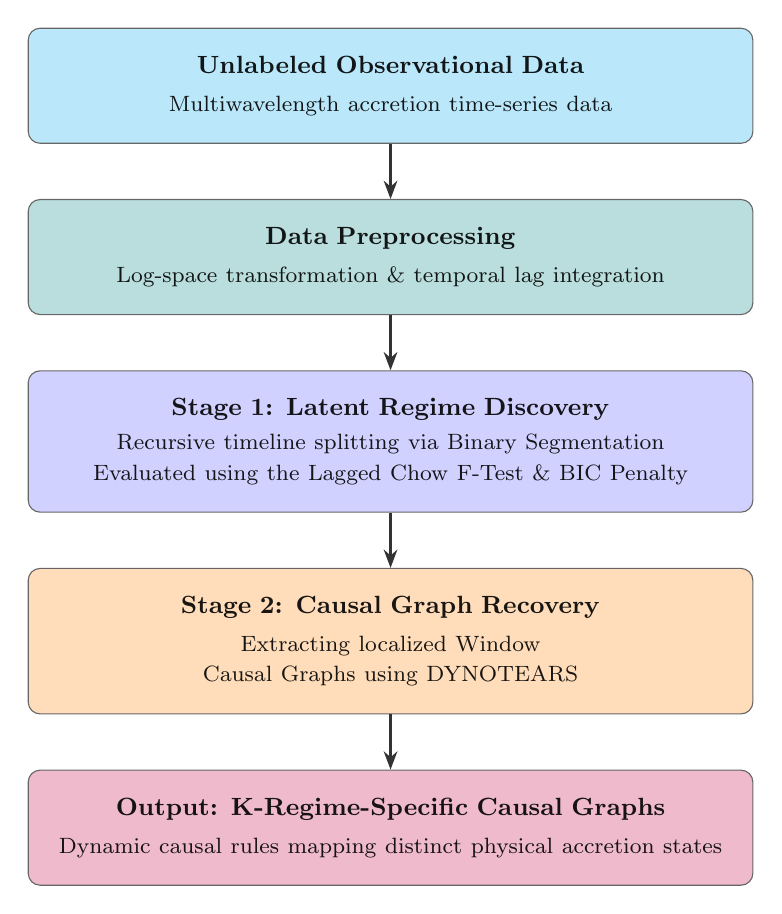
\begin{tikzpicture}[
        node distance=0.7cm,
        every node/.style={align=center, font=\small},
        outerbox/.style={draw=black!60, rectangle, rounded corners=1ex, inner sep=10pt, text width=8.5cm, fill opacity=0.9},
        arrow/.style={->, >=Stealth, thick, draw=black!80}
    ]

    % 1. Data Node
    \node[outerbox, fill=cyan!30] (data) {\textbf{Unlabeled Observational Data} \\ \vspace{0.3em} \footnotesize Multiwavelength accretion time-series data};

    % 2. Prep Node
    \node[outerbox, fill=teal!30] (prep) [below=of data] {\textbf{Data Preprocessing} \\ \vspace{0.3em} \footnotesize Log-space transformation \& temporal lag integration};

    % 3. Stage 1 Node
    \node[outerbox, fill=blue!20] (stage1) [below=of prep] {\textbf{Stage 1: Latent Regime Discovery} \\ \vspace{0.3em} \footnotesize Recursive timeline splitting via Binary Segmentation \\ \footnotesize Evaluated using the Lagged Chow F-Test \& BIC Penalty};

    % 4. Stage 2 Node
    \node[outerbox, fill=orange!30] (stage2) [below=of stage1] {\textbf{Stage 2: Causal Graph Recovery} \\ \vspace{0.3em} \footnotesize Extracting localized Window Causal Graphs using DYNOTEARS};

    % 5. Output Node
    \node[outerbox, fill=purple!30] (output) [below=of stage2] {\textbf{Output: K-Regime-Specific Causal Graphs} \\ \vspace{0.3em} \footnotesize Dynamic causal rules mapping distinct physical accretion states};

    % Main Vertical Arrows
    \draw[arrow] (data) -- (prep);
    \draw[arrow] (prep) -- (stage1);
    \draw[arrow] (stage1) -- (stage2);
    \draw[arrow] (stage2) -- (output);

    \end{tikzpicture}
    \caption{High-level pipeline of the unsupervised dynamic causal discovery framework, illustrating the progression from observational data to regime-specific causal graphs.}
    \label{fig:pipeline_intro}
\end{figure}
\vspace{1.5em}

\section{Scopes and Challenges}
This study combines causal inference with high-energy observational astrophysics.
The framework is designed for multi-wavelength black-hole accretion data and uses
log-linear structural equations within each regime. Its outputs are regime-specific
causal graphs, regression coefficients, and autoregressive parameters.

Several limitations remain. The linear model may miss nonlinear relationships, and
the piecewise-stationary model is only an approximation to continuous accretion
dynamics. The Chow test and BIC derivations assume Gaussian noise. The temporal
model uses only one lag, and the current validation uses synthetic rather than real
observations. Unmeasured variables, such as magnetic-field geometry, may create
spurious associations that the PC algorithm cannot resolve without additional
knowledge \cite{spirtes2000causation}. Residual autocorrelation may also inflate the
Chow statistic; Newey-West standard errors \cite{newey1987} are considered as a
robustness check. Non-Gaussian noise and violations of faithfulness provide further
challenges for causal discovery.


\chapter{Literature Review}
This chapter introduces the background needed to understand the method and results. It covers black hole accretion physics, time-series causal discovery, regime detection, and unsupervised clustering. It then reviews related studies and identifies the research gaps addressed by this thesis.

\section{Preliminaries}
The analysis combines two areas: black hole accretion physics and time-series causal discovery. The physical background explains why the Hard State and Soft State have different observational signatures. The statistical background explains how to model autocorrelation, hidden regime boundaries, and unknown state counts. This section introduces time-series concepts, causal inference, structural causal models, and the main tools used by the framework: OLS, the Chow test, binary segmentation, BIC, and DYNOTEARS.

\subsection{Multivariate Time-Series and Non-Stationarity}

\subsubsection*{i. Time Series Data}

Time-series data consist of observations collected at ordered time points. The order is part of the information in the data. A multivariate series can be written as $X = \{x_1, x_2, x_3, \dots, x_n\}$, where $n$ variables are measured over $T$ time steps \cite{assaad2022survey}. A variable at time $t$ may depend on variables from the same time step or on earlier observations. These past effects are called lagged effects. Because an infinite lag window is not practical, causal discovery uses a maximum lag, denoted by $I_{max}$.

\subsubsection*{ii. Stationary and Non-Stationary Data}

In stationary data, properties such as the mean and variance remain stable over time. In non-stationary data, these properties change, either gradually or at particular points.

\subsubsection*{iii. Temporal Regime}

A temporal regime is a consecutive time window in which the statistical properties or causal structure remain stable. If the properties are stable from $t=1$ to $t=m$ and change at $t=m+1$, the first interval forms one regime and the later stable interval up to $t=k$ forms another.

\subsubsection*{iv. Strict Stationary Assumption}

Many traditional models assume that the data-generating rules remain unchanged at every time step. This makes the time index independent of the data distribution and implies one causal structure for the whole series. The assumption is often unrealistic for dynamic systems. If the distribution or causal relationships change, a single stationary model can produce inaccurate or misleading discoveries.

\subsection{Black Holes and Accretion}

\subsubsection*{i. Black Holes}

Black holes are well-studied astrophysical objects, although many aspects of their behaviour remain uncertain.

A black hole is a region of spacetime from which light cannot escape after crossing the event horizon. Black holes are detected indirectly through their gravitational and electromagnetic effects on nearby matter. They can form when a massive star collapses. In general relativity, the event horizon marks the boundary beyond which information cannot return to an external observer.

For a non-rotating black hole, the radius of the event horizon is described by Equation~\eqref{eq:ch2-schwarzschild}:

\begin{equation}
    \label{eq:ch2-schwarzschild}
    R_s = \frac{2GM}{c^2}
\end{equation}

where $G$ is the gravitational constant, $M$ is the black-hole mass, and $c$ is the speed of light. At this radius, the escape velocity reaches the speed of light. The black hole itself does not emit electromagnetic radiation, but nearby matter can become very bright through \textit{accretion}.

\subsubsection*{ii. Accretion and Accretion Disks}

Accretion is the process by which matter is captured and moves toward a black hole. Because the matter has angular momentum, it usually forms a rotating flow instead of falling directly inward. Gravitational potential energy is converted into motion, heat, and radiation. Accretion is therefore one of the most efficient known mechanisms of energy release \cite{shakura1973, frank2002}.

As matter approaches a black hole, it forms a rotating accretion disk. Viscosity removes orbital energy and causes the gas to spiral inward. The resulting friction heats the disk to very high temperatures.

The disk is not equally hot at all radii. The outer region is cooler, while the inner region can emit strongly in X-rays. This emission provides information about the disk geometry and its behaviour.

\subsubsection*{iii. Black Hole X-ray Binaries}

Black holes are commonly grouped as \textit{stellar-mass}, \textit{intermediate-mass}, or \textit{supermassive}. Stellar-mass black holes in binary systems are common in the Milky Way. These systems are called Black Hole X-ray Binaries (BHXBs).

In a BHXB, the black hole orbits a companion star and pulls gas from it. The captured gas feeds the accretion disk. These systems allow rapid changes in accretion to be observed over weeks or months \cite{remillard2006, done2007}.
\subsubsection*{iv. Active Galactic Nuclei (AGN)}

\textit{Active Galactic Nuclei (AGN)} are powered by accretion onto supermassive black holes at the centres of galaxies. These black holes can be millions or billions of times more massive than the Sun.

The basic accretion physics is similar to that of stellar-mass black holes, but the larger mass produces much longer variability timescales. BHXBs can therefore serve as faster systems for studying accretion processes.

\subsubsection*{v. Accretion States}

Black holes do not accrete at a constant rate. They move between \textit{accretion states}, in which the flow geometry and energy-release mechanism change. The states are identified from their emitted spectra.

\subsubsection*{vi. Hard State}

In the \textit{Hard State}, the accretion rate is usually lower. The inner disk is often \textit{truncated} and replaced by a hot, diffuse gas cloud called a \textit{corona}.

A steady \textit{radio jet} is a key feature of this state. The observed emission is dominated by high-energy (\textit{Hard}) X-rays and often varies rapidly.

\subsubsection*{vii. Soft State}

At a higher accretion rate, the system can enter the \textit{Soft State}. The disk then extends inward to the closest stable orbit.

In the Soft State, the radio jet is \textit{quenched} or absent. The emission is dominated by thermal disk radiation and appears as a \textit{Soft} X-ray spectrum. Thus, the Soft State is disk-dominated, while the Hard State is jet-dominated.

\subsubsection*{viii. Power-Law Scaling Relations}

In contrast to the intricate physics of plasma dynamics and magnetic fields, the systems surrounding black holes exhibit a notable level of order. They adhere to Power-Law Scaling Relations. One physical feature (like brightness) is proportional to another raised to a specific exponent, $y = A x^k$.

In science, power laws are often a sign of scale \textit{invariance}. This suggests that the same physical law applies whether the black hole is small or supermassive. For the purpose of this research, these relations are very important because power laws become linear when converted to a logarithmic scale ($\log y = k \log x + \log A$). This makes them ideal for the causal discovery methods explored here.

\subsubsection*{ix. Fundamental Plane of Black Hole Activity}

The \textit{Fundamental Plane of Black Hole Activity} is a specific scaling relation that serves as a "universal rulebook" for black hole physics \cite{merloni2003}. It connects three core properties: Radio luminosity ($L_R$), X-ray luminosity ($L_X$), and the mass of the black hole ($M_{BH}$). Empirical observations indicate that the physical processes involved in accretion and jet production are similar over several orders of magnitude in mass:

Equation~\eqref{eq:ch2-fp-power} gives the power-law form:
\begin{equation}
    \label{eq:ch2-fp-power}
    L_R \propto L_X^{\xi_X} M_{BH}^{\xi_M}
\end{equation}

This relation is expressed logarithmically in Equation~\eqref{eq:ch2-fp-log}:

\begin{equation}
    \label{eq:ch2-fp-log}
    \log L_R = a \log L_X + b \log M_{BH} + c
\end{equation}

\subsection{Fundamentals of Causal Inference}

\textit{To understand the mechanisms governing each temporal regime, we rely on the formal framework of causal inference. This section introduces the necessary graphical and structural definitions, adopting the framework detailed by Neal (2020).}

\subsubsection*{i. Directed Acyclic Graphs (DAGs)}

A \textit{graph} is a mathematical structure consisting of a set of \textit{nodes} (or vertices) and a set of \textit{edges}, where each edge represents a relationship between two nodes. In the context of causal inference, nodes represent the variables or features of the dataset \cite{neal2020}.

In a \textit{directed graph}, edges contain arrows indicating the direction of the relationship. The node from which an edge originates is called the \textit{parent} node, and the node the edge points to is called the \textit{child} node. 

A \textit{path} is a sequence of nodes connected by edges, regardless of the direction of the arrows. A \textit{directed path}, however, is a sequence of nodes connected by directed edges that all point in the same forward direction. 

For a given node $X$, its \textit{descendants}, denoted as $de(X)$, consist of all nodes $Y$ for which there exists a directed path from $X$ to $Y$ (this includes children, children of children, and so forth). 
Conversely, the \textit{ancestors} of $Y$, denoted as $an(Y)$, consist of all nodes $X$ for which there exists a directed path from $X$ to $Y$ (including parents, parents of parents, etc.).

A \textbf{Directed Acyclic Graph (DAG)} is a directed graph that contains no \textit{cycles}; namely, there does not exist any directed path that starts and ends at the same node. Consequently, no node can be an ancestor or descendant of itself \cite{neal2020}.

\subsubsection*{ii. Causal Graphs}

A variable $X$ is considered a \textit{cause} of a variable $Y$ if an intervention or deliberate change in $X$ results in a change in the distribution of $Y$; this underlying mechanism is referred to as \textit{causation} \cite{neal2020}.

Within the framework of a directed graph, the \textit{Causal Edges Assumption} states that every parent node is a direct cause of all its child nodes. 

Consequently, a \textbf{Causal Graph} is formally defined as a Directed Acyclic Graph (DAG) that strictly satisfies the Causal Edges Assumption. In such a graph, every directed path from one node to another implies a flow of causation.

\subsubsection*{iii. Statistical Independence and Dependence}

Two random variables $X$ and $Y$ are \textbf{statistically independent} (or marginally independent), denoted as $X \perp\!\!\!\perp Y$, if their joint probability satisfies Equation~\eqref{eq:ch2-independence}:
\begin{equation}
    \label{eq:ch2-independence}
    P(X=x, Y=y) = P(X=x)P(Y=y)
\end{equation}
If this equality does not hold for at least one pair of $(x, y)$, the variables are \textbf{statistically dependent}, denoted as $X \not\perp\!\!\!\perp Y$, implying that observing the value of $X$ provides information that changes the probability of $Y$.

In real-life systems, variables are rarely entirely independent. Instead, we rely on \textbf{conditional independence}. Two random variables $X$ and $Y$ are conditionally independent given a third variable (or set of variables) $Z$, denoted as $X \perp\!\!\!\perp Y \mid Z$, if Equation~\eqref{eq:ch2-cond-independence} holds:
\begin{equation}
    \label{eq:ch2-cond-independence}
    P(X=x, Y=y \mid Z=z) = P(X=x \mid Z=z)P(Y=y \mid Z=z)
\end{equation}
In causal terms, conditional independence implies that once $Z$ is known, observing $X$ provides no additional information about $Y$ \cite{wasserman2004}.

\subsubsection*{iv. d-Separation and the Flow of Association}

In a causal graph, it is necessary to understand the conditional independence or dependence between two nodes. This criterion is known as \textbf{d-separation} (directional separation) \cite{neal2020}. 

Two nodes $X$ and $Y$ are d-separated by a set of conditioning nodes $Z$ if all paths between $X$ and $Y$ are mathematically blocked by $Z$. If $X$ and $Y$ are d-separated in the graph $\mathcal{G}$, it implies they are conditionally independent in the probability distribution: $X \perp\!\!\!\perp Y \mid Z$. Note that $Z$ is a set of nodes which can be empty.

To determine whether a specific path is open or blocked, we evaluate the path using three structural building blocks \cite{neal2020}:

\begin{quote}
\textbf{1. Chains (Mediation)}\\
A chain represents a sequence where causation flows through an intermediate variable ($X \rightarrow Z \rightarrow Y$). Here, $X$ is a cause of $Z$, and $Z$ is a cause of $Y$.
This path is by default open and $X$ and $Y$ are statistically dependent. However, conditioning on the mediator $Z$ blocks the flow of association. 
\textit{Example:} In urban infrastructure, heavy rain ($X$) causes waterlogging ($Z$), which subsequently causes severe traffic gridlock ($Y$). Conditioning on the waterlogging ($Z$) mathematically blocks the association between heavy rain and traffic gridlock.

\begin{center}
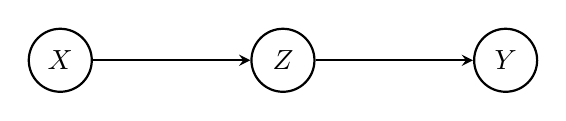
\begin{tikzpicture}[->, >=stealth, thick, node distance=2cm]
    \node[circle, draw, minimum size=0.8cm] (X) {$X$};
    \node[circle, draw, minimum size=0.8cm] (Z) [right=of X] {$Z$};
    \node[circle, draw, minimum size=0.8cm] (Y) [right=of Z] {$Y$};
    \draw (X) -- (Z);
    \draw (Z) -- (Y);
\end{tikzpicture}
\end{center}
\end{quote}

\begin{quote}
\textbf{2. Forks (Confounding)}\\
A fork happens when a single variable is the common cause of two separate variables ($X \leftarrow Z \rightarrow Y$). Here, $Z$ is a cause of both $X$ and $Y$.
This path is open by default, introducing confounding bias. Conditioning on the common cause $Z$ blocks this spurious flow of association.
\textit{Example:} A summer heatwave ($Z$) simultaneously causes load-shedding ($X$) and an increase in app-based ride demand ($Y$). Conditioning on the temperature ($Z$) d-separates the electricity usage from the ride-hailing demand, removing the fake correlation between load-shedding ($X$) and app-based ride demand ($Y$).

\begin{center}
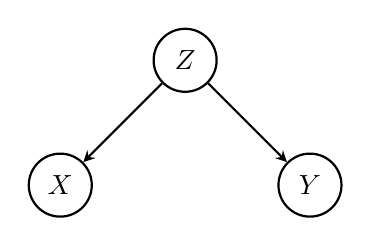
\begin{tikzpicture}[->, >=stealth, thick, node distance=2cm]
    \node[circle, draw, minimum size=0.8cm] (Z) {$Z$};
    \node[circle, draw, minimum size=0.8cm] (X) [below left=1cm and 1cm of Z] {$X$};
    \node[circle, draw, minimum size=0.8cm] (Y) [below right=1cm and 1cm of Z] {$Y$};
    \draw (Z) -- (X);
    \draw (Z) -- (Y);
\end{tikzpicture}
\end{center}
\end{quote}

\begin{quote}
\textbf{3. Colliders (Selection Bias)}\\
A collider exists when two independent variables have a common effect ($X \rightarrow Z \leftarrow Y$). Here, both $X$ and $Y$ are causes of $Z$. If $X$ and $Y$ are not directly connected by an edge, this specific V-structure is formally known as an \textit{immorality}. 
Unlike chains and forks, a collider naturally blocks the flow of association. However, conditioning on the collider $Z$ (or any of its descendants) opens a spurious path between $X$ and $Y$. 
\textit{Example:} In an academic environment, consider the factors for getting a good grade in a certain course ($Z$). A student's prior foundational knowledge ($X$) and their dedicated study hours ($Y$) independently increase the probability of securing an 'A'. Prior knowledge and study hours might be independent; however, if a researcher restricts their analysis to students who actually received an 'A' (conditioning on the collider $Z$), they will induce a spurious negative correlation. Within this conditioned group, a student without prior foundational knowledge must have compensated with a high number of study hours to achieve the grade. This creates a mathematically false implication that having stronger foundational knowledge causes a student to study less. 

\begin{center}
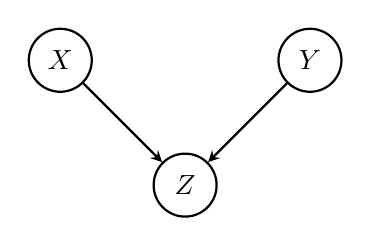
\begin{tikzpicture}[->, >=stealth, thick, node distance=2cm]
    \node[circle, draw, minimum size=0.8cm] (Z) {$Z$};
    \node[circle, draw, minimum size=0.8cm] (X) [above left=1cm and 1cm of Z] {$X$};
    \node[circle, draw, minimum size=0.8cm] (Y) [above right=1cm and 1cm of Z] {$Y$};
    \draw (X) -- (Z);
    \draw (Y) -- (Z);
\end{tikzpicture}
\end{center}
\end{quote}

Formally, a path between nodes $A$ and $B$ is blocked (no flow of association) by a conditioning set $M$ if at least one of the following conditions is met \cite{neal2020}:
\begin{enumerate}
    \item The path contains a chain ($X \rightarrow Y \rightarrow Z$) or a fork ($X \leftarrow Y \rightarrow Z$) such that the middle node $Y$ is in the conditioning set $M$.
    \item The path contains a collider ($X \rightarrow Y \leftarrow Z$) such that the middle node $Y$ is \textit{not} in $M$, and no descendant of $Y$ is in $M$.
\end{enumerate}

\subsubsection*{v. Structural Causal Models (SCMs)}

A \textbf{Structural Causal Model (SCM)} is a mathematical framework used to model cause-and-effect relations in an environment \cite{neal2020}. While a DAG is the visual description of causality, an SCM provides the mathematical rules for those relations. 

In an SCM, every single node is calculated through the function in Equation~\eqref{eq:ch2-scm}:
\begin{equation}
    \label{eq:ch2-scm}
    X_i := f_i(\text{PA}(X_i), \epsilon_i)
\end{equation}
where: 
\begin{itemize}
    \item $X_i$ (The effect): The variable being calculated.
    \item $\text{PA}(X_i)$ (The causes): The set of parents of $X_i$ which are causing the effect.
    \item $f_i$ (The function): The deterministic mathematical relation that computes the effect from the causes.
    \item $\epsilon_i$ (The noise term): The variation in the effect that the causes \textit{cannot} explain.
    \item $:=$ (The assignment): The mathematical assignment operation means $X_i$ is defined by the right-hand side. Note that this operation is not symmetric. 
\end{itemize}

To illustrate how a DAG translates into structural mathematical equations, consider a system with the causal structure: $A \rightarrow C$, $B \rightarrow C$, $B \rightarrow D$, $D \rightarrow E$, and $E \rightarrow F$.

\begin{center}
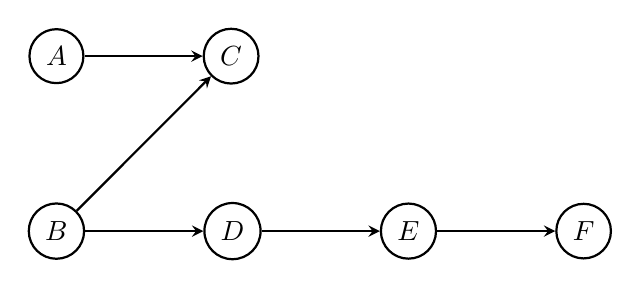
\begin{tikzpicture}[->, >=stealth, thick, node distance=1.5cm]
    \node[circle, draw] (A) {$A$};
    \node[circle, draw] (B) [below=of A] {$B$};
    \node[circle, draw] (C) [right=of A] {$C$};
    \node[circle, draw] (D) [right=of B] {$D$};
    \node[circle, draw] (E) [right=of D] {$E$};
    \node[circle, draw] (F) [right=of E] {$F$};
    \draw (A) -- (C);
    \draw (B) -- (C);
    \draw (B) -- (D);
    \draw (D) -- (E);
    \draw (E) -- (F);
\end{tikzpicture}
\end{center} 

The corresponding SCM defines each node as a deterministic function of its direct parents and its unobserved noise ($\epsilon$): 
\begin{align*}
A &:= f_A(\epsilon_A) \\
B &:= f_B(\epsilon_B) \\
C &:= f_C(A, B, \epsilon_C) \\
D &:= f_D(B, \epsilon_D) \\
E &:= f_E(D, \epsilon_E) \\
F &:= f_F(E, \epsilon_F)
\end{align*}

In this structure, nodes $A$ and $B$ have no direct parents (they act as root nodes), meaning their assignments rely entirely on their respective noise terms. Node $C$, acting as a collider between $A$ and $B$, takes both parent variables as arguments in its structural function.

\subsubsection*{vi. The Discovery Postulates: Markov and Faithfulness}

Every mathematical field stands on axioms and postulates. Similarly, to successfully discover a causal graph $\mathcal{G}$ from the probability distribution $P$ of observational data, it is necessary to establish a mathematical bridge between the SCM and statistical independence. This bridge relies on two foundational postulates: the \textbf{Causal Markov Assumption} and the \textbf{Faithfulness Assumption} \cite{neal2020}.

\begin{quote}
\textbf{1. The Local Causal Markov Assumption} (Equation~\eqref{eq:ch2-markov})\\
The Causal Markov Assumption dictates that a node is conditionally independent of all its non-descendants, given its direct parents. Formally, for any node $X$ in a DAG $\mathcal{G}$, where $\text{PA}(X)$ represents its parents and $\text{ND}(X)$ represents its non-descendants:
\begin{equation}
    \label{eq:ch2-markov}
    X \perp\!\!\!\perp \text{ND}(X) \mid \text{PA}(X)
\end{equation}
This assumption guarantees that the causal graph naturally imposes the correct conditional independencies on the joint probability distribution. If two variables are d-separated in the graph $\mathcal{G}$, they \textit{must} be statistically independent in the data $P$.
\end{quote}

\begin{quote}
\textbf{2. The Faithfulness Assumption}\\
The Faithfulness Assumption is the logical converse of the Markov Assumption. A probability distribution $P$ is considered faithful to a DAG $\mathcal{G}$ if \textit{every} conditional independence observed in the data is strictly the result of a structural d-separation in the graph.
Formally, if $X \perp\!\!\!\perp Y \mid Z$ is found in the data distribution $P$, then $X$ and $Y$ must be d-separated by $Z$ in $\mathcal{G}$. This axiom ensures that two causal paths do not perfectly and coincidentally cancel each other out to create a fake statistical independence.
\end{quote}

Together, these postulates guarantee that the structural d-separations in the causal graph perfectly map to the statistical conditional independencies in the observable time-series data, making the unsupervised discovery of the DAG mathematically possible.


\subsection{Unsupervised Learning and Clustering}

\textit{Because the structural boundaries of real-world temporal regimes are rarely known in advance, discovering these shifts requires analyzing the data without predefined labels. This section discusses the application of clustering and temporal segmentation to identify these hidden causal boundaries.}

\subsubsection*{i. The Need for Unsupervised Learning}

We have theoretically established the basic theoretical framework for modeling causal structure. In this section, we address a major methodological challenge of causal modeling, which is detecting the temporal regimes without knowing the structural boundaries of the data. We frame this as an unsupervised learning problem. In traditional supervised learning algorithms, models are trained with data with input features $x$ where the actual outputs $y$ are known beforehand. But in most real-life dynamic systems, it is not feasible to gather the predefined target outputs. So, the exact boundaries of the temporal regimes stay hidden. Supervised learning cannot work in this case. To solve this, we rely on unsupervised learning, which seeks to recover latent structure without reference to known or labeled outcomes \cite{hastie2009}. Since our multivariate time-series data does not contain the predefined labels, it is mandatory to use unsupervised learning to discover the underlying Structural Causal Model (SCM) shifts.

\subsubsection*{ii. Clustering vs. Temporal Segmentation}

One of the primary techniques for unsupervised learning is the method of clustering. In this method, the data are grouped in a way such that the intra-group similarity is maximized and the inter-group similarity is minimized. One such well-known clustering technique is k-means clustering. In this method, data points are assigned to clusters based entirely on their feature proximity, ignoring the sequence of the data. So, applying standard clustering on time-series data where the sequence matters destroys the temporal precedence required for causal discovery. To solve this problem, we can use temporal segmentation. Temporal segmentation safeguards continuity by grouping contiguous time blocks into discrete clusters. Here, each cluster represents a temporal regime, and the boundary between two regimes is now clearly defined, which our causal model may work with \cite{assaad2022survey}. 

To illustrate this within a real-world context, consider the highly dynamic environmental and traffic conditions of Dhaka City. A multivariate time-series dataset tracking hourly parameters, such as traffic density, weather metrics (humidity, wind speed), and air quality markers like PM2.5, exhibits distinct, unlabeled temporal regimes. During the Winter Regime (November-February), cold weather and stagnant air mean traffic density has a strong, direct causal link to sudden PM2.5 spikes. However, during the Monsoon Regime (June-August), heavy rainfall washes away pollutants, breaking or heavily weakening that direct causal link, while the rain itself becomes the primary cause of traffic gridlock. Standard clustering like k-means would completely ignore this and may group data based only on features like traffic speed, which may cluster winter data and summer data together. Temporal segmentation, however, treats winter and monsoon as continuous, separate blocks of time with their own distinct causal behaviors.

\subsubsection*{iii. Requirements for Temporal Segmentation}

Although there exist many algorithms which may be used to perform temporal segmentation, some rules or requirements have to be enforced for our specific problem.

\begin{itemize}
    \item \textbf{Contiguity enforcement:} The algorithm must ensure that each cluster is an unbroken sequence of time. 
    \item \textbf{Dynamic graph optimization:} The cluster fit shouldn't just be the distance between two data points, but also how a Directed Acyclic Graph (DAG) explains the entire block of data. 
    \item \textbf{Complexity penalization:} The algorithm might assign each time-step its own unique regime which we have to prevent. We can prevent it by ensuring that some penalty term is added to the objective function which balances the accuracy of the causal graph against the number of structural breaks. 
\end{itemize}

By satisfying the requirements, the unsupervised algorithm can successfully divide the non-stationary time-series data into unique stationary regimes, which will allow the discovery of a DAG within each time block.


\subsection{Dynamic Causal Models and Time-Series Graphs}

In a standard Structural Causal Model (SCM), cause-and-effect relationships are captured only at a single, isolated instant. The underlying mathematics cannot account for historical dependencies, and a traditional DAG is limited to representing static relations. To evaluate dynamical systems, causal influences from the past must be explicitly taken into account. Therefore, to properly study structural breaks across temporal regimes, we must shift from the standard causal framework introduced in the previous section to Dynamic Causal Models.

\subsubsection*{i. Unrolling the Graph over Time (Dynamic Bayesian Networks)}

A Dynamic Bayesian Network (DBN) is a directed graphical representation of a stochastic process \cite{murphy2012}. It is important to note that the network structure itself is not dynamic; rather, it is a fixed topology that models variables across discrete slices of time. By unrolling these static time slices, the network formally represents a dynamical system capable of accounting for historical dependencies. 

To rigorously define a DBN, three structural requirements must be specified \cite{murphy2012}:
\begin{enumerate}
    \item \textbf{The Initial State:} The structural topology of the first time-slice ($t = 0$).
    \item \textbf{The Transition Model:} The directed connections between historical time-slices ($t - \tau$) and the current time-slice ($t$).
    \item \textbf{The Probability Distributions:} The specific Conditional Probability Distributions (CPDs) that mathematically govern the relations along these directed connections.
\end{enumerate}

\subsubsection*{ii. Defining Time-Series Causal Graphs}

To apply causal discovery algorithms to time-series data, we must mathematically formalize how the unrolled Dynamic Bayesian Network is represented as a graph. Depending on the level of temporal detail required, time-series causality can be represented using three distinct graphical definitions \cite{assaad2022survey}. These representations are illustrated in Figure~\ref{fig:timeseries-graphs}:

\begin{quote}
\textbf{1. The Full Time Causal Graph}\\
The Full Time Causal Graph captures all causal relations throughout all possible time. This is an infinite Directed Acyclic Graph (DAG) where every variable at every time step is denoted by an independent node.  
Formally, the set of nodes is defined as $\{X_t^i \mid \forall i, \forall t \}$. An edge drawn from $X_{t-\tau}^j \rightarrow X_t^i$ indicates a direct causal relationship with an exact time delay of $\tau$. If $\tau = 0$, the edge represents a contemporaneous effect; if $\tau > 0$, the edge represents a lagged effect. 
Although this graph contains all the theoretical information, the sheer number of nodes and edges makes it computationally intractable for causal discovery algorithms.   
\end{quote}

\begin{quote}
\textbf{2. The Window Causal Graph}\\
Because the Full Time Causal Graph is computationally intractable, we must compress the temporal information into a manageable window. As a result, this graph restricts the analysis to a specific, finite maximum time lag, denoted as $\tau_{max}$. 
In this representation, an edge $X_{t-\tau}^j \rightarrow X_t^i$ is only valid and included in the graph if the delay is within the sliding window ($\tau \leq \tau_{max}$). This operates under the assumption that an effect past $\tau_{max}$ is negligible and is instead mediated by more recent causal relations. The Window Causal Graph is the primary target structure for time-series causal discovery algorithms and is the most prominent representation utilized in this thesis. 
\end{quote}

\begin{quote}
\textbf{3. The Summary Causal Graph}\\
Unlike the Full Time Causal Graph or the Window Causal Graph, the Summary Causal Graph does not incorporate timestamps; it serves as a full summary of the entire temporal history, containing information across all time steps. In this graph, nodes revert to their static definitions ($X^i$ and $X^j$, dropping the time index $t$). 
An edge $X^j \rightarrow X^i$ is drawn if there exists \textit{any} time delay $\tau \geq 0$ where $X_{t-\tau}^j$ causes $X_t^i$ in the underlying full graph. Because this aggregation ignores the strict forward-flowing direction of time, a Summary Causal Graph can contain cycles ($X^j \rightarrow X^i$ and $X^i \rightarrow X^j$ can simultaneously exist if they occur at different lags). Therefore, unlike a standard static causal graph, a Summary Causal Graph is not necessarily a DAG.
\end{quote}

\begin{figure}[h!]
\centering
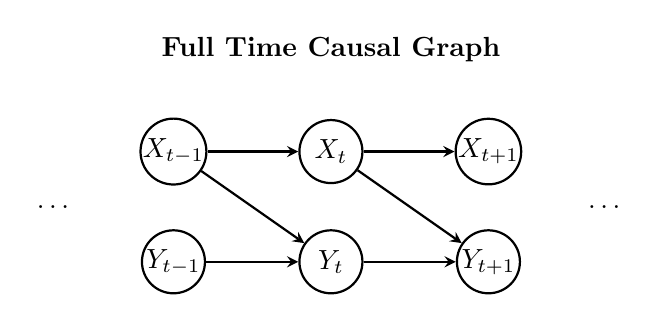
\begin{tikzpicture}[->, >=stealth, thick, node distance=1.5cm]
    % Full Time Causal Graph
    \node (FT_title) at (3.5, 2) {\textbf{Full Time Causal Graph}};
    \node (t0) at (0,0) {\dots};
    \node[circle, draw, minimum size=0.8cm, inner sep=0pt] (X1) at (1.5, 0.7) {$X_{t-1}$};
    \node[circle, draw, minimum size=0.8cm, inner sep=0pt] (Y1) at (1.5, -0.7) {$Y_{t-1}$};
    \node[circle, draw, minimum size=0.8cm, inner sep=0pt] (X2) at (3.5, 0.7) {$X_{t}$};
    \node[circle, draw, minimum size=0.8cm, inner sep=0pt] (Y2) at (3.5, -0.7) {$Y_{t}$};
    \node[circle, draw, minimum size=0.8cm, inner sep=0pt] (X3) at (5.5, 0.7) {$X_{t+1}$};
    \node[circle, draw, minimum size=0.8cm, inner sep=0pt] (Y3) at (5.5, -0.7) {$Y_{t+1}$};
    \node (t4) at (7,0) {\dots};

    \draw (X1) -- (X2); \draw (X2) -- (X3);
    \draw (Y1) -- (Y2); \draw (Y2) -- (Y3);
    \draw (X1) -- (Y2); \draw (X2) -- (Y3);
\end{tikzpicture}

\vspace{1cm}

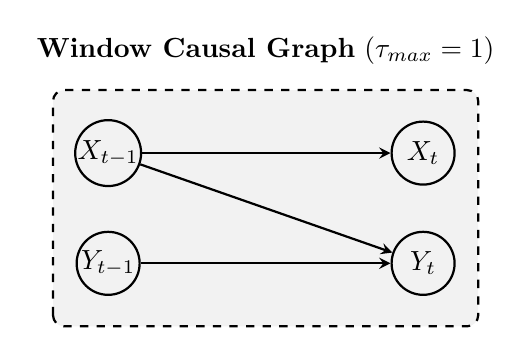
\begin{tikzpicture}[->, >=stealth, thick, node distance=1.5cm]
    % Window Causal Graph
    \node (W_title) at (2, 2) {\textbf{Window Causal Graph} ($\tau_{max} = 1$)};
    \draw[dashed, fill=gray!10, rounded corners] (-0.7, -1.5) rectangle (4.7, 1.5);
    \node[circle, draw, minimum size=0.8cm, inner sep=0pt] (X1) at (0, 0.7) {$X_{t-1}$};
    \node[circle, draw, minimum size=0.8cm, inner sep=0pt] (Y1) at (0, -0.7) {$Y_{t-1}$};
    \node[circle, draw, minimum size=0.8cm, inner sep=0pt] (X2) at (4, 0.7) {$X_{t}$};
    \node[circle, draw, minimum size=0.8cm, inner sep=0pt] (Y2) at (4, -0.7) {$Y_{t}$};
    \draw (X1) -- (X2);
    \draw (Y1) -- (Y2);
    \draw (X1) -- (Y2);
\end{tikzpicture}

\vspace{1cm}

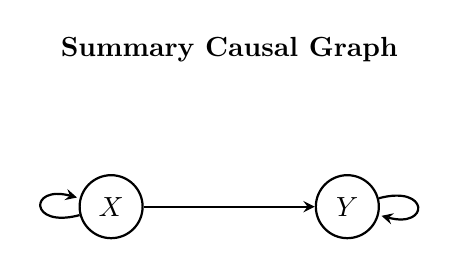
\begin{tikzpicture}[->, >=stealth, thick, node distance=2cm]
    % Summary Causal Graph
    \node (S_title) at (1.5, 2) {\textbf{Summary Causal Graph}};
    \node[circle, draw, minimum size=0.8cm] (X) at (0, 0) {$X$};
    \node[circle, draw, minimum size=0.8cm] (Y) at (3, 0) {$Y$};
    \draw (X) edge[loop left] (X);
    \draw (Y) edge[loop right] (Y);
    \draw (X) -- (Y);
\end{tikzpicture}
\caption{Representations of Time-Series Causal Graphs}
\label{fig:timeseries-graphs}
\end{figure}

By understanding these three representations, we can define unsupervised clustering algorithms to discover distinct temporal regimes in a time-series by analyzing localized Window or Summary Causal Graphs.

\subsubsection*{iii. The Time-Series Structural Causal Model}

A standard Structural Causal Model (SCM) assumes all variables operate within the same isolated instant. However, in a Time-Series Structural Causal Model, we must extend this framework to account for the flow of time $t$.

In a time-series SCM, a variable is not merely caused by other variables, but by specific historical time instants (from $t-1$ down to $t - \tau_{max}$) of those variables \cite{assaad2022survey}. Equation~\eqref{eq:ch2-timeseries-scm} formally defines a time-series SCM:

\begin{equation}
    \label{eq:ch2-timeseries-scm}
    X_t^i := f_i( \{ X_{t-\tau}^j \mid X_{t-\tau}^j \in \text{PA}(X_t^i) \}, \epsilon_t^i )
\end{equation}

where:
\begin{itemize}
    \item $X_t^i$ (The present effect): The target variable being calculated at the current time step $t$.
    \item $\text{PA}(X_t^i)$ (The temporal parents): The set of all direct causes of $X_t^i$. Because time is now a factor, this set can contain two distinct types of causes:
    \begin{itemize}
        \item \textbf{Contemporaneous Effects:} Causes that occur within the exact same time step ($\tau = 0$), denoted as $X_t^j \rightarrow X_t^i$.
        \item \textbf{Time-Lagged Effects:} Causes that occurred in the strict past ($\tau > 0$), denoted as $X_{t-\tau}^j \rightarrow X_t^i$. Note that a variable can be a lagged cause of itself ($X_{t-\tau}^i \rightarrow X_t^i$), representing auto-correlation.
    \end{itemize}
    \item $f_i$: The deterministic function mapping the historical and instantaneous parents to the current effect.
    \item $\epsilon_t^i$: The independent noise term at time $t$.
\end{itemize}

To illustrate how a static DAG is unrolled into this time-series SCM format (using a maximum time lag of $\tau_{max} = 2$), consider a dynamic system with three variables ($A$, $B$, and $C$). Let the causal structure dictate the following temporal rules: $A$ influences its own next state, $A$ influences $B$ with a delay of two time steps, $B$ influences its own next state, $A$ influences $C$ with a delay of one time step, and $B$ influences $C$ instantaneously.

\begin{center}
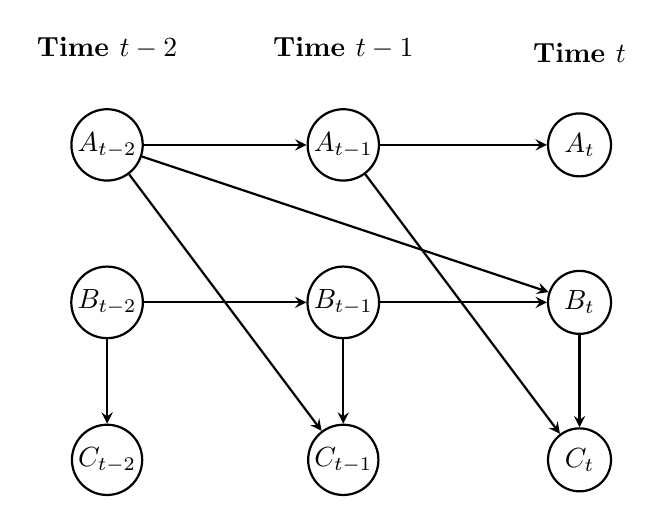
\begin{tikzpicture}[->, >=stealth, thick, node distance=2cm]
    % time t-2
    \node[circle, draw, inner sep=1pt, minimum size=0.8cm] (A2) at (0, 2) {$A_{t-2}$};
    \node[circle, draw, inner sep=1pt, minimum size=0.8cm] (B2) at (0, 0) {$B_{t-2}$};
    \node[circle, draw, inner sep=1pt, minimum size=0.8cm] (C2) at (0, -2) {$C_{t-2}$};

    % time t-1
    \node[circle, draw, inner sep=1pt, minimum size=0.8cm] (A1) at (3, 2) {$A_{t-1}$};
    \node[circle, draw, inner sep=1pt, minimum size=0.8cm] (B1) at (3, 0) {$B_{t-1}$};
    \node[circle, draw, inner sep=1pt, minimum size=0.8cm] (C1) at (3, -2) {$C_{t-1}$};

    % time t
    \node[circle, draw, inner sep=1pt, minimum size=0.8cm] (A0) at (6, 2) {$A_{t}$};
    \node[circle, draw, inner sep=1pt, minimum size=0.8cm] (B0) at (6, 0) {$B_{t}$};
    \node[circle, draw, inner sep=1pt, minimum size=0.8cm] (C0) at (6, -2) {$C_{t}$};

    % Column labels
    \node[above=0.5cm of A2, font=\bfseries] {Time $t-2$};
    \node[above=0.5cm of A1, font=\bfseries] {Time $t-1$};
    \node[above=0.5cm of A0, font=\bfseries] {Time $t$};

    % Rules applied sequentially to represent DBN
    % A auto-correlation
    \draw (A2) -- (A1);
    \draw (A1) -- (A0);
    
    % B auto-correlation
    \draw (B2) -- (B1);
    \draw (B1) -- (B0);
    
    % A influences B with lag 2
    \draw (A2) -- (B0);
    
    % A influences C with lag 1
    \draw (A2) -- (C1);
    \draw (A1) -- (C0);
    
    % B influences C instantaneously
    \draw (B2) -- (C2);
    \draw (B1) -- (C1);
    \draw (B0) -- (C0);

\end{tikzpicture}
\end{center} 

The corresponding time-series equations dictate the state of each node at the current time step $t$:

\begin{align*}
A_t &:= f_A(A_{t-1}, \epsilon_{A,t}) \\
B_t &:= f_B(B_{t-1}, A_{t-2}, \epsilon_{B,t}) \\
C_t &:= f_C(B_t, A_{t-1}, \epsilon_{C,t})
\end{align*}

In this dynamic system, the equation for $A_t$ demonstrates a lagged auto-correlation ($\tau = 1$), the equation for $B_t$ demonstrates a cross-lagged effect reaching back to the maximum lag limit ($\tau = 2$), and the equation for $C_t$ demonstrates a combination of a historical effect from $A$ ($\tau = 1$) and a contemporaneous effect from $B$ ($\tau = 0$).

\subsubsection*{iv. Consistency Throughout Time and Structural Breaks}

The mathematical formalizations of Time-Series SCMs and Window Causal Graphs rely on a fundamental assumption: the underlying causal mechanisms do not change spontaneously or erratically. It is highly unlikely that a causal direction will abruptly flip within a stable window; if such instability occurred frequently, the system would fragment into countless micro-regimes, causing the predictive model to collapse. In most macroscopic real-world scenarios, a causal link from $A$ to $B$ might weaken or disappear over time, but an immediate reversal where $B$ suddenly causes $A$ is highly improbable. This principle of stability is formally known as \textbf{Consistency Throughout Time}.

According to Assaad et al. \cite{assaad2022survey}, a time-series causal graph is consistent throughout time if the presence and direction of every causal edge remain invariant across all time steps. For instance, if $X$ causes $Y$ with a lag of $\tau = 1$ at time $t$, it must also cause $Y$ with the exact same lag at time $t+100$. 

In the context of this thesis, Consistency Throughout Time serves as the core defining characteristic of a \textbf{Temporal Regime}. As long as the consistency of the causal graph remains unbroken, that contiguous block of time constitutes a single, independent regime. 

However, in real-world dynamical systems, environments evolve and underlying rules change. When this consistency assumption is violated over time—for example, when an existing causal edge disappears or a new one emerges—we denote that exact moment as a \textbf{Structural Break}. Consequently, the time steps following this break transition into an entirely different regime. In observational data, this often manifests as certain variables becoming causally isolated while new cause-and-effect relationships are born.

To illustrate this dynamically, we extend the Dhaka City environmental model introduced in Section 2.1.4. Consider a multivariate time-series dataset tracking hourly parameters: Traffic Density ($X$), PM2.5 levels ($Y$), and Rainfall ($Z$). 

\begin{itemize}
    \item \textbf{Regime 1: The Winter Consistency (Nov--Feb):} Cold weather and stagnant air mean traffic density has a strong, direct causal link to sudden PM2.5 spikes. During this contiguous block of time, the Window Causal Graph maintains a perfectly consistent, lagged edge: $X_{t-\tau} \rightarrow Y_t$.
    \item \textbf{The Structural Break:} As the climate shifts, the environmental physics governing the city fundamentally change. The consistency assumption is violated.
    \item \textbf{Regime 2: The Monsoon Consistency (Jun--Aug):} Heavy rainfall washes away pollutants, effectively breaking the direct causal link from traffic to air quality. Simultaneously, the rain itself becomes the primary cause of traffic gridlock. The old causal edge ($X_{t-\tau} \rightarrow Y_t$) disappears from the Window Causal Graph, replaced by a newly consistent edge representing the rain's effect on traffic ($Z_{t-\tau} \rightarrow X_t$).
\end{itemize}

Because the exact temporal boundary (the structural break) between these distinct causal regimes is hidden within the unlabeled observational data, we cannot rely on supervised learning to locate it. This dictates the core methodological approach of this thesis: we must treat the discovery of these structural breaks as an \textbf{unsupervised learning} problem, utilizing clustering algorithms to segment the time-series based solely on the shifting structures of the underlying Window Causal Graphs.


\subsection{Algorithmic Framework for Regime Detection and Causal Discovery}

Identifying independent temporal regimes, and more precisely, locating their underlying structural breaks require a multi-step pipeline. Therefore, our methodology relies on the integration of multiple algorithms, analytical tools, and optimization techniques. Within this pipeline, the time-series data is first segmented into distinct temporal regimes, and subsequently, the specific causal structure of each isolated regime is extracted. To achieve this, our framework relies on three core stages:

\subsubsection*{i. Parameter Estimation and Model Scoring}
\begin{itemize}
    \item \textbf{Ordinary Least Squares (OLS):} OLS serves as the baseline optimization technique in this framework. It mathematically estimates the strength of the relationship (the edge weight) between a historical cause and a present effect. Because these cause-and-effect relationships are temporal, the true edge weights remain constant within a stable regime but shift when a structural break occurs. By minimizing the residual sum of squares, OLS evaluates the baseline error for any given window of time.  
    \item \textbf{Bayesian Information Criterion (BIC):} BIC acts as the penalized scoring metric for this framework. During clustering, if every tiny chunk of time were segmented independently, the OLS error would drop to near zero, but the model would severely overfit, rendering the results meaningless. BIC introduces a mathematical penalty for each new regime discovered. Consequently, it balances the need to minimize OLS error against model complexity, ensuring the algorithm does not fracture the timeline into an excessive and insignificant number of segments.  
\end{itemize}

This fundamental trade-off between minimizing OLS error and minimizing the BIC penalty ensures the mathematical foundation necessary to deploy search algorithms to locate the exact structural breaks.

\subsubsection*{ii. Structural Break Identification}
To identify the exact temporal boundaries where structural breaks occur, we utilize recursive hypothesis testing driven by OLS error evaluation.

\begin{itemize}
    \item \textbf{Binary Segmentation (BinSeg):} Because a time-series may contain multiple hidden regimes, evaluating every single time step independently for a structural break is computationally intractable. To optimize this, we employ Binary Segmentation, a recursive "divide-and-conquer" search strategy. At each step, the algorithm sweeps the current time window, identifies the single point with the highest Chow Test significance score, and divides the data at that exact juncture. The recursion then continues independently on those newly divided sub-segments. Furthermore, because the true number of regimes is unknown, this method is highly advantageous; it iteratively halves the timeline only when statistically justified, isolating independent regimes without requiring a predefined regime count.  
    \item \textbf{Chow F-Test:} The Chow F-Test serves as the statistical engine that dictates whether BinSeg should actually execute a split. It evaluates if a structural break is genuinely happening by comparing the OLS error of a single continuous time window against the combined OLS error of the two segments proposed by BinSeg. If formulating two distinct regression models significantly reduces the overall residual error, the Chow Test mathematically confirms that a structural break has occurred and the regime has shifted.
\end{itemize}

\subsubsection*{iii. Continuous Causal Graph Discovery}
Once the entire time-series is segmented into independent regimes, the final step is to discover the internal dynamic causal graph governing each regime. 

\begin{itemize}
    \item \textbf{The DYNOTEARS Algorithm:} Traditional causal discovery algorithms, such as the PC algorithm, rely on combinatorial graph search and do not scale well with dense time-series data. To extract the causal relations and underlying structures from each independent regime, we utilize DYNOTEARS, a temporal extension of the NOTEARS framework. DYNOTEARS advances DAG learning by replacing discrete graph search with a continuous, differentiable optimization problem. This formulation allows the algorithm to efficiently learn both instantaneous and lagged causal effects simultaneously. By applying DYNOTEARS individually to each temporal block isolated by BinSeg, we can extract the exact localized Window Causal Graph for that specific regime.
\end{itemize}

\subsubsection*{iv. Summary and Baseline Assumptions}
In summary, this pipeline functions as a comprehensive framework for unsupervised causal inference: OLS measures the baseline error, BIC prevents model overfitting, Binary Segmentation recursively divides the timeline, the Chow F-Test statistically validates the structural breaks, and finally, DYNOTEARS maps the dynamic causal graphs. 

It must be noted that this baseline framework initially operates under the assumption of linear causal relationships. If real-world datasets exhibit strong non-linear mechanisms, the performance of this specific configuration may degrade. However, because this pipeline is inherently modular, each algorithm or statistical test can be substituted with non-linear alternatives optimized for the target dataset. Consequently, this architecture can be adapted to capture the behaviors of highly complex dynamic systems.












% ============================================================

\section{Causal Discovery and Time Series: Progress and Key Findings}
\label{sec:survey}

Causal discovery has developed from classical graphical models into methods that
handle mixed data, heterogeneity, and temporal dependence. Recent work focuses on
nonstationary and high-dimensional time series.

\subsection{Graphical Causal Discovery}

The main classical approaches are constraint-based methods, such as PC and FCI,
and score-based DAG learning. These methods provide the theoretical basis for
structure learning, but their reliability can decrease with nonlinearity,
measurement error, nonstationarity, and latent confounding
\cite{glymour2019review}. Hybrid approaches combine the strengths of both families.
For example, constraint-based filtering can reduce the search space before Bayesian
sampling is applied \cite{kuipers2018efficient}.

Recent methods also address mixed data and larger graphs. Likelihood-ratio tests
improve conditional-independence testing for mixed variables
\cite{tsagris2018constraint}, while variational Bayesian methods improve scalability
\cite{annadani2021variational}. Other work studies assumption violations
\cite{faltenbacher2025internal}, cyclic graphs \cite{mooij2020fci}, joint graph and
effect uncertainty \cite{castelletti2021structural}, and NOTEARS-style learning for
mixed data \cite{zhao2024notearsm}.

\subsection{Heterogeneity, Non-stationarity, and Mechanism Shifts}

Changes across environments can provide information about causal direction. CD-NOD
uses distribution shifts to recover causal structure from heterogeneous or
nonstationary data \cite{huang2020causal}. The Sparse Mechanism Shift hypothesis
shows that a full graph can become identifiable when only a small number of causal
mechanisms change across environments \cite{perry2022causal}.

Recent methods also cluster observations by their causal mechanisms. HCL learns
latent clusters and their graphs from mixed observational data without environment
labels \cite{li2025hcl}. MCVCI and MCVCC extend this idea to mixtures of bivariate
mechanisms \cite{liu2025hybrid}. These methods motivate the present work, which
considers unknown regime counts and sequential observations.

\subsection{Causal Discovery for Time Series (Stationary and Non-stationary)}

Time-series causal discovery includes Granger-based, constraint-based, noise-based,
score-based, logic-based, topology-based, and difference-based methods
\cite{assaad2022survey}. No family is best in every setting. Each depends on
assumptions such as linearity, causal sufficiency, stationarity, or acyclicity.
Multivariate time series add further problems, including subsampling and unmeasured
confounding \cite{glymour2019review}.

CD-NOTS extends CD-NOD to nonstationary time series
\cite{sadeghi2025causal,huang2020causal}. It models contemporaneous and lagged
effects while enforcing consistency across time. It also corrects problems that can
arise when lagged variables are used in conditional-independence tests. The method
supports KCIT, RCoT, CMIknn, and ParCorr, allowing the test to be selected for the
sample size and dimensionality. Its financial-data experiments show that
nonstationary and nonlinear effects can be missed by stationary linear methods.

\subsection{Deep-learning and Granger-based Methods}
\label{ssec:granger}

Deep-learning methods extend Granger-based discovery to larger and more complex
time series. TCDF uses an attention-based temporal CNN and permutation validation
to learn graphs and lags \cite{nauta2019causal}. NTiCD combines LSTMs with graph
convolutions \cite{absar2023neural}. CUTS+ uses Granger-based neural components
with graph neural networks for irregular streams \cite{cheng2023cuts}. Transformer
attention has also been used to represent changing Granger graphs
\cite{zhu2025attention}. These approaches depend on temporal ordering and therefore
do not directly apply to unordered i.i.d. observations.

\subsection{Temporal Causal Discovery with Unknown Regimes: CASTOR}

CASTOR is the closest existing method to this thesis. It learns causal graphs from
multivariate time series with an unknown number of sequential regimes
\cite{rahmani2025castor}. It estimates the regime count, the boundaries, and the
causal DAG for each regime.

CASTOR uses expectation-maximisation. The E-step updates regime-membership
probabilities, while the M-step estimates a BIC-penalised DAG under the NOTEARS
acyclicity constraint \cite{zheng2018dags}. It starts with equal-width windows and
merges adjacent windows with similar causal structures. The method provides
identifiability results under Gaussian equal-variance noise. Experiments on graphs
with up to 40 nodes and two real benchmarks report improvements over CD-NOD,
RPCMCI, and DYNOTEARS in regime recovery and graph recovery.

CASTOR and LIRA address the same broad problem: finding an unknown number of
sequential regimes and their graphs without environment labels. Their boundary
criteria differ. CASTOR accepts boundaries through a global EM and BIC objective.
LIRA first applies a Chow $F$-test to ask whether the coefficient vectors differ,
then uses BIC to control model complexity. This gives a statistical test and a
separate parsimony check for each candidate boundary.

LIRA also uses a domain-specific structural model derived from the Fundamental
Plane of Black Hole Activity. This fixes the variable set and gives the model
parameters a physical interpretation. CASTOR is domain-agnostic and therefore more
general. In return, LIRA uses stronger physical assumptions. Its greedy binary
segmentation may miss jointly detectable boundaries, and its piecewise-constant
model cannot represent gradual changes. These limitations motivate future
comparisons with CASTOR and DyCAST.

\subsection{Continuously Evolving Causal Structure: DyCAST}

DyCAST models causal structure as a continuous function of time rather than as a
sequence of fixed regimes \cite{cheng2025dycast}. Neural ODEs constrained to the
DAG manifold allow it to represent smooth transitions. Experiments on synthetic,
fMRI, CausalTime, and motion-capture data show strong performance and better
scaling than several static temporal methods. However, DyCAST also requires
temporal ordering and therefore is not a direct solution for unordered data.

\subsection{Challenges and Methodological Themes}

The performance of causal discovery depends strongly on whether the model
assumptions match the data \cite{assaad2022survey}. Important challenges include
nonlinearity, causal insufficiency, mixed data types, high dimensionality, and
finite-sample error. Existing responses include hybrid Bayesian learning
\cite{kuipers2018efficient}, mixed-data independence tests
\cite{tsagris2018constraint}, and graph neural networks for coarse-to-fine discovery
\cite{cheng2023cuts}.

The field is also moving toward uncertainty quantification. Variational causal
networks estimate distributions over possible DAGs \cite{annadani2021variational},
and joint graph-effect models propagate structural uncertainty into effect estimates
\cite{castelletti2021structural}. Validation is another growing focus, with evidence
that learned Granger graphs can improve forecasting \cite{zhang2023causalformer}.

\subsection{Conclusion of the Survey}

Causal discovery now includes methods for mixed data, heterogeneity, uncertainty,
and temporal dynamics. However, each method depends on particular assumptions.
Many approaches require environment labels, an auxiliary time or domain index, or
temporal ordering. This thesis focuses on discovering causal regimes from
unlabelled observations while estimating the number of regimes and testing whether
their mechanisms differ. CASTOR provides the closest temporal analogue, but its
dependence on sequential regime assignment does not solve this problem directly.

The main related methods are compared in Table~\ref{tab:related_works}.
\newcolumntype{P}[1]{>{\raggedright\arraybackslash}p{#1}}

{\small
\renewcommand{\arraystretch}{1.3}
\begin{longtable}{|P{2.0cm}|P{2.3cm}|P{2.5cm}|P{1.8cm}|P{4.3cm}|}
\caption{Summary of major related works in causal discovery, regime detection,
and causal clustering.}
\label{tab:related_works} \\
\hline
\textbf{Study} & \textbf{Task} & \textbf{Method} & \textbf{Setting} & \textbf{Main Finding / Gap} \\
\hline
\endfirsthead

\multicolumn{5}{c}%
{{\bfseries \tablename\ \thetable{} -- continued from previous page}} \\
\hline
\textbf{Study} & \textbf{Task} & \textbf{Method} & \textbf{Setting} & \textbf{Main Finding / Gap} \\
\hline
\endhead

\hline \multicolumn{5}{|r|}{{Continued on next page}} \\ \hline
\endfoot

\hline
\endlastfoot

Spirtes et al.\ \cite{spirtes2000causation}
& DAG learning from observational data
& PC and FCI constraint-based algorithms
& i.i.d., single environment
& Foundational framework for causal discovery. Assumes a single fixed causal model throughout. \\
\hline
Zheng et al.\ \cite{zheng2018dags}
& Continuous DAG structure learning
& NOTEARS: smooth algebraic acyclicity constraint
& i.i.d., single environment
& Enables gradient-based DAG learning at scale. The acyclicity constraint underpins DYNOTEARS and CASTOR. \\
\hline
Pamfil et al.\ \cite{pamfil2020dynotears}
& Time-series causal graph recovery
& DYNOTEARS: NOTEARS extended to contemporaneous and lagged edges
& Stationary time series
& Efficiently recovers window causal graphs. Assumes stationarity holds throughout the entire series. \\
\hline
Huang et al.\ \cite{huang2020causal}
& Causal discovery under heterogeneity
& CD-NOD: nonparametric method exploiting distribution shifts
& Multiple domains or time-indexed data
& Heterogeneity aids causal identification. Requires an auxiliary domain index or time stamp. \\
\hline
Peters et al.\ \cite{peters2016causal}
& Causal parent identification
& ICP: invariant prediction across environments
& Multiple labelled environments
& Exploits causal invariance effectively. Requires environment labels as a strict prerequisite. \\
\hline
Arjovsky et al.\ \cite{arjovsky2019irm}
& Out-of-distribution generalisation
& IRM: invariant risk minimisation
& Multiple labelled environments
& Encourages causally stable features. Guarantees weaken when the environment count is small. \\
\hline
Perry et al.\ \cite{perry2022causal}
& Multi-environment causal graph recovery
& Sparse Mechanism Shift hypothesis with MSS score
& Multiple labelled environments
& Full graph identifiable under sparse shifts. Environment membership must still be known. \\
\hline
Huang et al.\ \cite{huang2019specific}
& Causal clustering with shared and specific relations
& SSCM: mixture of causal mechanisms
& i.i.d., multiple regimes
& Distinguishes shared and regime-specific causal relations. Requires a pre-specified regime count. \\
\hline
Chen et al.\ \cite{chen2023ccsl}
& Causal structure learning from unknown environments
& CCSL: Bayesian nonparametric Causal CRP with variational inference
& i.i.d., unknown environments
& Does not require a regime count in advance. Identifiable under a linear non-Gaussian assumption. Primary baseline for this thesis. \\
\hline
Varambally et al.\ \cite{varambally2024mcd}
& Mixture of causal models from time series
& MCD: variational inference over mixtures of SCMs
& Temporal, autoregressive structure
& Jointly infers causal models and mixing probabilities. Relies on temporal ordering. \\
\hline
Rahmani and Frossard \cite{rahmani2025castor}
& Temporal causal regime discovery
& CASTOR: EM over piecewise-constant regimes with NOTEARS acyclicity
& Sequential time series
& Jointly learns regime boundaries and per-regime DAGs without a prior regime count. Relies on temporal contiguity unavailable in i.i.d.\ settings. \\
\hline
Cheng et al.\ \cite{cheng2025dycast}
& Continuously evolving causal structure
& DyCAST: Neural ODE constrained to DAG manifold
& Sequential time series
& Captures smooth causal transitions and scales beyond 50 nodes. Requires temporal ordering. \\
\hline
Li et al.\ \cite{li2025hcl}
& Unsupervised causal clustering from mixed-type data
& HCL: bi-directional iterative causal clustering (preprint)
& i.i.d., no environment labels
& No temporal ordering or regime count required. Scalability on large graphs has not yet been assessed. \\
\hline
Sadeghi et al.\ \cite{sadeghi2025causal}
& Causal discovery from nonstationary time series
& CD-NOTS: nonparametric extension of CD-NOD correcting lagged conditioning
& Non-stationary time series
& Uncovers nonlinear nonstationary causal relations missed by stationarity-assuming methods. \\
\hline
Mooij et al.\ \cite{mooij2020jci}
& Joint causal inference from multiple contexts
& JCI: context encoded as additional graph nodes
& Multiple pre-specified contexts
& Theoretically general and subsumes many special cases. Contexts must be labelled in advance. \\
\hline
Faltenbacher et al.\ \cite{faltenbacher2025internal}
& Assumption violation detection
& Internal incoherency scores for constraint-based algorithms
& i.i.d., single environment
& Flags assumption violations without ground truth. Not yet adapted to causal clustering settings. \\
\hline

\end{longtable}
}


\section{Foundations of Causal Discovery}
\label{sec:foundations}

Causal discovery infers causal relationships from observational data. Constraint-based
methods, such as PC and FCI, use conditional-independence tests. PC returns a
Markov equivalence class of DAGs, while FCI also allows latent confounding and
returns a partial ancestral graph \cite{spirtes2000causation}.

Score-based methods search for a DAG that fits the data well. GES performs a greedy
search over equivalence classes. NOTEARS reformulates DAG learning as continuous
optimization by expressing acyclicity as a smooth constraint
\cite{zheng2018dags}. DYNOTEARS extends this formulation to contemporaneous and
lagged relationships in time series \cite{pamfil2020dynotears}.

Functional causal models make stronger assumptions about the functional form and
noise distribution. LiNGAM can identify the causal order when the model is linear
and the noise is non-Gaussian \cite{shimizu2006lingam}. VAR-LiNGAM extends this
idea to vector autoregressive models with instantaneous and lagged effects
\cite{hyvarinen2010estimation}.

These foundational methods generally assume one causal model for the full dataset.
Real data may combine several latent processes, populations, time intervals, or
biological states. A single model fitted to such data can produce an averaged graph
that represents none of the underlying mechanisms. This motivates methods for
heterogeneous structure learning.

\subsection{Causal Discovery from Nonstationary and Heterogeneous Data}
\label{ssec:nonstationary}

Several methods use changes across environments to improve causal identification.
Invariant Causal Prediction identifies parents whose conditional relationship with a
target remains stable across known environments \cite{peters2016causal}. Its main
limitation is the need for environment labels.

CD-NOD uses distribution shifts across domains or time to recover causal structure
\cite{huang2020causal}. It needs an auxiliary domain or time index, but not hard
environment labels. CD-NOTS adapts this idea to time series and improves the
treatment of lagged variables \cite{sadeghi2025causal}. The Sparse Mechanism Shift
hypothesis gives theoretical support to this approach when only a few mechanisms
change \cite{perry2022causal}.

DyCAST models continuous changes in the causal DAG with Neural ODEs
\cite{cheng2025dycast}. IRM provides a related learning-theoretic approach that
encourages stable predictors across environments \cite{arjovsky2019irm}. Both IRM
and ICP require known environment partitions.

Together, these studies show that heterogeneity can help causal learning. However,
existing methods generally need environment labels, an auxiliary nonstationarity
index, or temporal ordering. Recovering regimes without all three is the central gap
addressed by this thesis.

\subsection{Mixture Models and Causal Clustering}
\label{ssec:clustering}

Causal clustering jointly estimates cluster assignments and causal structures. This
is preferable to a sequential approach because incorrect assignments can corrupt
graph learning, while an incorrect graph can corrupt clustering.

The Specific and Shared Causal Model (SSCM) represents data as a mixture of causal
mechanisms and separates shared from regime-specific relations
\cite{huang2019specific}. It requires the number of regimes in advance.

CCSL is more flexible. It uses a causal Chinese Restaurant Process to group
observations by causal-structure similarity rather than feature distance
\cite{chen2023ccsl}. Variational inference estimates the parameters and assignments
together, and the number of groups need not be supplied. CCSL provides
identifiability under a linear non-Gaussian model and has been tested on fMRI and
Sachs protein-signalling data.

\subsubsection*{i. Temporal Extensions of Causal Clustering}

MCD learns mixtures of structural causal models from time series using variational
inference \cite{varambally2024mcd}. Its autoregressive structure makes it unsuitable
for i.i.d. cross-sectional data. CASTOR provides a temporal method for jointly
learning sequential regimes and their DAGs \cite{rahmani2025castor}, but its use of
temporal contiguity does not transfer directly to unordered observations.

\subsubsection*{ii. i.i.d. Extensions and Recent Advances}

HCL jointly learns latent clusters and causal structures from mixed observational
data without environment labels or a pre-specified regime count
\cite{li2025hcl}. Its preprint reports weaker assumptions than CCSL, but its
identifiability conditions and large-graph performance require further study.
MCVCI and MCVCC show that mechanism-aware clustering is also useful in simple
bivariate mixtures \cite{liu2025hybrid}.

\subsubsection*{iii. Classical Clustering Methods}

Methods such as k-means, GMM, DBSCAN, and OPTICS group observations by similarity
in feature space. They can fail when regimes have similar distributions but
different causal mechanisms. CCSL results show the value of including causal
structure in the clustering objective \cite{chen2023ccsl}.

\subsection{Joint Causal Inference from Multiple Contexts}

JCI represents contexts as additional nodes in a causal graph and learns causal
structure across observational and interventional settings \cite{mooij2020jci}.
It is general, but the contexts must be known in advance. Representation-learning
methods also study hidden causal variables, but they usually focus on learning
latent variables from images or videos rather than grouping tabular observations by
causal regime.

\section{Summary of Key Findings}
\label{sec:summary}

The literature has moved from single-environment causal discovery to methods that
use known environments, distribution shifts, or joint causal clustering. This
section summarises the main trends and limitations and states the gaps addressed by
this thesis.

\subsection{Methodological Trends}

Constraint-based methods use conditional independence, while score-based methods
optimize a graph score such as BIC. Functional causal models, including LiNGAM and
VAR-LiNGAM, use stronger assumptions about the noise and functional form
\cite{assaad2022survey,shimizu2006lingam,hyvarinen2010estimation}.

In heterogeneous settings, invariance and distribution shifts are the main guiding
ideas. They appear in ICP, CD-NOD, CD-NOTS, IRM, and JCI
\cite{peters2016causal,huang2020causal,sadeghi2025causal,arjovsky2019irm,mooij2020jci}.
CASTOR and DyCAST model temporal changes as piecewise-constant or continuously
evolving structures \cite{rahmani2025castor,cheng2025dycast}. Causal clustering
methods such as SSCM, CCSL, HCL, and MCD jointly estimate assignments and causal
models \cite{huang2019specific,chen2023ccsl,li2025hcl,varambally2024mcd}.

\subsection{Consistent Findings}

The reviewed studies support five conclusions:
\begin{enumerate}[nosep]
\item Causal structure can differ substantially across regimes. A pooled model can
produce a graph that represents none of them
\cite{huang2020causal,chen2023ccsl,varambally2024mcd,li2025hcl,rahmani2025castor}.
\item Joint estimation of assignments and causal structures is generally better than
a sequential pipeline \cite{huang2019specific,chen2023ccsl,li2025hcl,rahmani2025castor}.
\item Causal-structure similarity can be a better clustering signal than feature
distance or correlation \cite{chen2023ccsl}.
\item Real data often violates stationarity, as shown by CD-NOTS and CASTOR
\cite{sadeghi2025causal,rahmani2025castor}.
\item No method is universally best. Performance depends on whether its assumptions
match the data-generating process \cite{assaad2022survey}.
\end{enumerate}

\subsection{Contradictions and Limitations}

ICP and IRM require known environment partitions. CD-NOD and CD-NOTS require an
auxiliary domain or time index. CCSL assumes stationarity within clusters, while
CASTOR handles sequential changes but assumes piecewise-constant regimes and
Gaussian equal-variance noise. These requirements limit their use when the hidden
state and the number of regimes are both unknown.

There is also a trade-off between flexibility and identifiability. CCSL has formal
guarantees under linear non-Gaussian noise, but that assumption may be restrictive.
HCL and MCD use more flexible models but provide weaker or less developed formal
guarantees. Evaluation is also inconsistent: some studies report clustering quality
without graph quality, while others do the reverse. A common benchmark is still
needed. Internal incoherency scores are promising for detecting assumption
violations, but they have not been adapted to causal clustering
\cite{faltenbacher2025internal}.

\subsection{Research Gaps}
\label{ssec:gaps}

The main gaps relevant to this thesis are:
\begin{itemize}[leftmargin=1.4em]
\item \textbf{No formal invariance test for discovered boundaries.} CASTOR and
DyCAST use global optimization scores, but do not attach a direct hypothesis test
to each proposed boundary. LIRA addresses this with a Chow test followed by an
independent BIC decision.
\item \textbf{No formal test of structural difference.} Existing causal-clustering
methods generally do not test whether two learned regimes differ beyond finite-sample
variation.
\item \textbf{Limited scalability evidence.} Most causal-clustering studies use
small synthetic graphs. Comparable large-graph evaluations remain limited.
\item \textbf{No standard causal-clustering benchmark.} The field lacks agreed
datasets and evaluation measures for comparing regime recovery and graph recovery.
\item \textbf{Limited observational identifiability theory.} Formal guarantees for
mixtures of SCMs from observational i.i.d. data remain limited beyond the linear
non-Gaussian case of CCSL.
\item \textbf{Within-regime nonstationarity.} Most methods assume that each regime
is stationary, even though the mechanism may continue to change inside a regime.
\item \textbf{Assumption checks without ground truth.} Tools for detecting violated
causal assumptions have not been developed fully for causal clustering.
\end{itemize}

This thesis addresses the first two gaps directly and evaluates regime recovery,
graph recovery, and scalability on controlled synthetic data. The remaining gaps,
including standard benchmarks, within-regime nonstationarity, and broader
assumption checks, are left for future work.



\chapter{Requirements, Impacts and Constraints}
% \section{Final Specifications and Requirements}
% This section discusses technical or methodological Requirements, data or resource requirements (software), etc.

% \section{Societal Impact}
% Study and report on project impact on society, health, safety, legal, and cultural aspects.

% \section{Environmental Impact}
% Study and report on project sustainability and environmental impact.

% \section{Ethical Issues}
% Identify ethical issues and professional responsibilities related to the design solution.

% \section{Standards - if applicable}
% Write about any standard maintained.

\section{Project Management Plan}

The project is organised into three phases over 46 weeks. The schedules are shown
in Figures~\ref{fig:plan-phase1},~\ref{fig:plan-phase2}, and~\ref{fig:plan-phase3}.

The phases follow the order of the research process. Phase 1 establishes the physical
and methodological foundation. Phase 2 develops and tests the algorithms under
controlled conditions. Phase 3 applies the validated pipeline to real observations
and completes the reporting.

This order reduces the risk of interpreting real data with an untested method.

\vspace{0.5cm}
\textbf{Phase 1 (Weeks 1 to 15). Background and Method Design}

The first 15 weeks are reserved for background study and method design. The later
experiments depend on both of them.

The literature review is completed first so that the project requirements and research
gaps are clear. The clustering and causal discovery reviews come next. They are
followed by the accretion-disk review, which connects the statistical problem to the
physical variables.

The gaps found in these reviews guide the pipeline design. Data collection or
simulation is scheduled at the end of this phase. The data generator and preprocessing
choices should follow the final model design.

\vspace{0.5cm}
\begin{enumerate}
    \item Review causal discovery methods for time series.
    \item Review unsupervised methods for regime identification.
    \item Review accretion-disk physics and known accretion states.
    \item Identify gaps in causal discovery for astrophysical time series.
    \item Design the regime-separation and graph-recovery pipeline.
    \item Obtain or simulate accretion-disk time-series data from sources such as GRMHD simulations or NICER/RXTE archives.
\end{enumerate}

\vspace{0.5cm}
\begin{figure}[htbp]
\centering
\begin{center}
\begin{ganttchart}[
    x unit=0.8cm,
    y unit title=0.8cm,
    y unit chart=0.8cm,
    vgrid,
    hgrid,
    title label font=\bfseries\small,
    bar label font=\small,
    bar/.style={fill=blue!20},
    include title in canvas=false
]{1}{15}
\gantttitle{Phase 1. Weeks 1 to 15}{15} \\
\gantttitlelist{1,...,15}{1} \\
\ganttbar{Task 1}{1}{3} \\
\ganttbar{Task 2}{4}{6} \\
\ganttbar{Task 3}{7}{9} \\
\ganttbar{Task 4}{10}{11} \\
\ganttbar{Task 5}{12}{14} \\
\ganttbar{Task 6}{14}{15}
\end{ganttchart}
\end{center}
\caption{Project plan for Phase 1.}
\label{fig:plan-phase1}
\end{figure}
\vspace{0.5cm}

Figure~\ref{fig:plan-phase1} shows that the tasks are arranged from general to
specific. The first reviews establish the research context. The physics review and
gap analysis then define the scientific and technical requirements.

Pipeline design comes next, followed by data preparation. This sequence ensures that
the data and experiments match the proposed method rather than being selected
independently of it.

\vspace{0.5cm}
\textbf{Phase 2 (Weeks 16 to 30). Algorithm Development and Simulation}

Phase 2 uses 15 weeks to implement and test the method before real-data analysis.
The first step is to generate data with known regimes and graphs. Ground truth is
required for objective evaluation.

Regime clustering is implemented next. Graph recovery within each estimated regime
comes after it. Once both components are available, the complete pipeline can be
compared with the known ground truth.

The final weeks are used for sensitivity analysis. The method is tested under
different noise levels, sample sizes, and sampling patterns.

\vspace{0.5cm}
\begin{enumerate}
    \item Generate data with known causal graphs and regime labels.
    \item Implement regime clustering based on mechanism changes.
    \item Implement time-series causal discovery within each regime.
    \item Compare the recovered regimes and graphs with the ground truth.
    \item Test sensitivity to noise, sample size, and irregular sampling.
\end{enumerate}

\vspace{0.5cm}
\begin{figure}[htbp]
\centering
\begin{center}
\begin{ganttchart}[
    x unit=0.8cm,
    y unit title=0.8cm,
    y unit chart=0.8cm,
    vgrid,
    hgrid,
    title label font=\bfseries\small,
    bar label font=\small,
    bar/.style={fill=blue!20},
    include title in canvas=false
]{16}{30}
\gantttitle{Phase 2. Weeks 16 to 30}{15} \\
\gantttitlelist{16,...,30}{1} \\
\ganttbar{Task 1}{16}{18} \\
\ganttbar{Task 2}{19}{21} \\
\ganttbar{Task 3}{22}{25} \\
\ganttbar{Task 4}{26}{28} \\
\ganttbar{Task 5}{29}{30}
\end{ganttchart}
\end{center}
\caption{Project plan for Phase 2.}
\label{fig:plan-phase2}
\end{figure}
\vspace{0.5cm}

Figure~\ref{fig:plan-phase2} reflects this dependency. Data generation comes before
algorithm testing, and regime discovery comes before regime-specific graph learning.
Validation is scheduled only after the full pipeline is available.

Sensitivity analysis is last because it evaluates the stability of the completed
implementation.

\vspace{0.5cm}
\textbf{Phase 3 (Weeks 31 to 46). Real-Data Application and Reporting}

The final 16 weeks are used for real-data application and communication of the
results. Real light curves are analysed only after the synthetic tests. The synthetic
tests show that the method can recover known structures.

The discovered regimes are then compared with known accretion states. Their graphs
are examined for physical differences. The report is drafted after the main analysis.
It then reflects the final results and limitations.

Visualisation is completed at the end. It presents the regime assignments, graphs,
and time-series results consistently throughout the thesis.

\vspace{0.5cm}
\begin{enumerate}
    \item Apply the pipeline to real accretion-disk light curves, such as those from GRS 1915+105 or Cygnus X-1.
    \item Interpret the discovered regimes using known accretion states.
    \item Compare the causal graphs and discuss their physical meaning.
    \item Write the report, including the method, results, and limitations.
    \item Prepare causal graphs, regime assignments, and time-series plots.
\end{enumerate}

\vspace{0.5cm}
\begin{figure}[htbp]
\centering
\begin{center}
\begin{ganttchart}[
    x unit=0.75cm,
    y unit title=0.8cm,
    y unit chart=0.8cm,
    vgrid,
    hgrid,
    title label font=\bfseries\small,
    bar label font=\small,
    bar/.style={fill=blue!20},
    include title in canvas=false
]{31}{46}
\gantttitle{Phase 3. Weeks 31 to 46}{16} \\
\gantttitlelist{31,...,46}{1} \\
\ganttbar{Task 1}{31}{34} \\
\ganttbar{Task 2}{35}{37} \\
\ganttbar{Task 3}{38}{40} \\
\ganttbar{Task 4}{41}{44} \\
\ganttbar{Task 5}{45}{46}
\end{ganttchart}
\end{center}
\caption{Project plan for Phase 3.}
\label{fig:plan-phase3}
\end{figure}
\vspace{0.5cm}

Figure~\ref{fig:plan-phase3} shows this final progression. Real-data analysis begins
the phase. Interpretation follows the discovery of the regimes. Reporting begins
after the main findings are available.

The final visualization task supports the written discussion. It also prepares the
project for review and submission.

\section{Risk Management}

\vspace{0.3cm}
Real astrophysical time series, including X-ray light curves, can be noisy, irregular,
and limited in size. These properties make causal graph recovery and regime
separation difficult.

Unlike in a controlled experiment, the accretion state for each observation is not known.
The number of causal mechanisms is also uncertain. Unobserved variables, such as
magnetic-field changes, may confound the measured features.

Many causal discovery algorithms also assume acyclic relationships. Accretion disks
can contain feedback among temperature, density, and accretion rate.

The study manages these risks in three ways. First, it uses simulated data with known
graphs for controlled validation. Second, it uses methods designed for time series and
time-delayed effects. Third, it compares results across methods and tests their
stability under noise and small sample sizes.

\vspace{0.5cm}
\textbf{Risks of Synthetic Data}

Synthetic data is central to Phase 2. It is the only practical way to know the
correct regime boundaries and causal graphs in advance. Without a known answer, it is
impossible to say whether the pipeline recovered the true structure. It could also
have simply produced a plausible-looking result.

Synthetic data carries its own set of risks. These risks must be stated clearly.

The first risk is that the generator may be too favourable to the method. The
simulated series are built from the same linear and piecewise-stationary assumptions
that LIRA uses to recover them. If the real system departs from these assumptions,
the simulation results will overestimate performance.

To reduce this risk, the study varies noise levels, sample sizes, and sampling
patterns. It also compares the pipeline against established baselines rather than
against an empty model.

The second risk is that synthetic data does not contain every feature of real
observations. Real X-ray light curves contain gaps caused by telescope visibility.
They also contain instrumental artefacts and source-specific variability. A simple
generator does not reproduce these effects.

A method that works perfectly on clean simulations may fail when they are present.
The sensitivity analysis therefore includes irregular and noisy conditions. It cannot
cover every case that real data may present.

The third risk is overconfidence. Because the boundary and graph are known during
simulation, it is tempting to treat a successful recovery as proof that the method
works in general.

The study avoids this. Synthetic results are treated as a necessary but insufficient
condition. The pipeline must first succeed under controlled conditions. It is only
then applied to real observations where the truth is unknown.

Any claim from the synthetic experiments is a claim about the implementation. It is
not a claim about black hole physics.

The fourth risk is that the assumed collider structure may not hold for every
system. The identifiability analysis depends on this structure. If real accretion
variables form causal chains instead of the collider used here, the identifiability
guarantee does not transfer.

This limitation is carried forward into the discussion of real data in Chapter 6. It
is not hidden by the simulation.

This risk strategy also explains the phase order. Phase 1 reduces design risk through
background study and method specification. Phase 2 reduces implementation risk by
testing the pipeline where the correct answer is known. The synthetic-data risks
above are contained and documented in this phase.

Phase 3 addresses the remaining scientific risk. It applies the validated method to
real observations. It also reports the assumptions and uncertainties that cannot be
removed from observational data.

The phase order is therefore not only a schedule. It is a deliberate escalation from
low-risk controlled tests to high-risk real-data analysis. No stage begins before the
previous stage has established its own reliability.

% \section{Economic Analysis}
% Conduct economic analysis and cost-benefit estimation.



\chapter{Proposed Methodology}

\section{Overview}

The framework has four stages. \textbf{Stage 0} transforms the observables into log
space using the power-law structure of accretion. \textbf{Stage 1} finds regime
boundaries with recursive binary segmentation, a lagged Chow $F$-test, and BIC.
\textbf{Stage 2} estimates a dynamic causal graph for each regime with DYNOTEARS.
\textbf{Stage 3} validates the resulting causal effects.

The physical states are introduced first in Figure~\ref{fig:section-c-1}. Their
hypothesised causal structures are then shown in Figure~\ref{fig:section-c-2}. The
complete recursive pipeline appears in Figure~\ref{fig:pipeline}.

\begin{figure}[htbp]
    \centering
    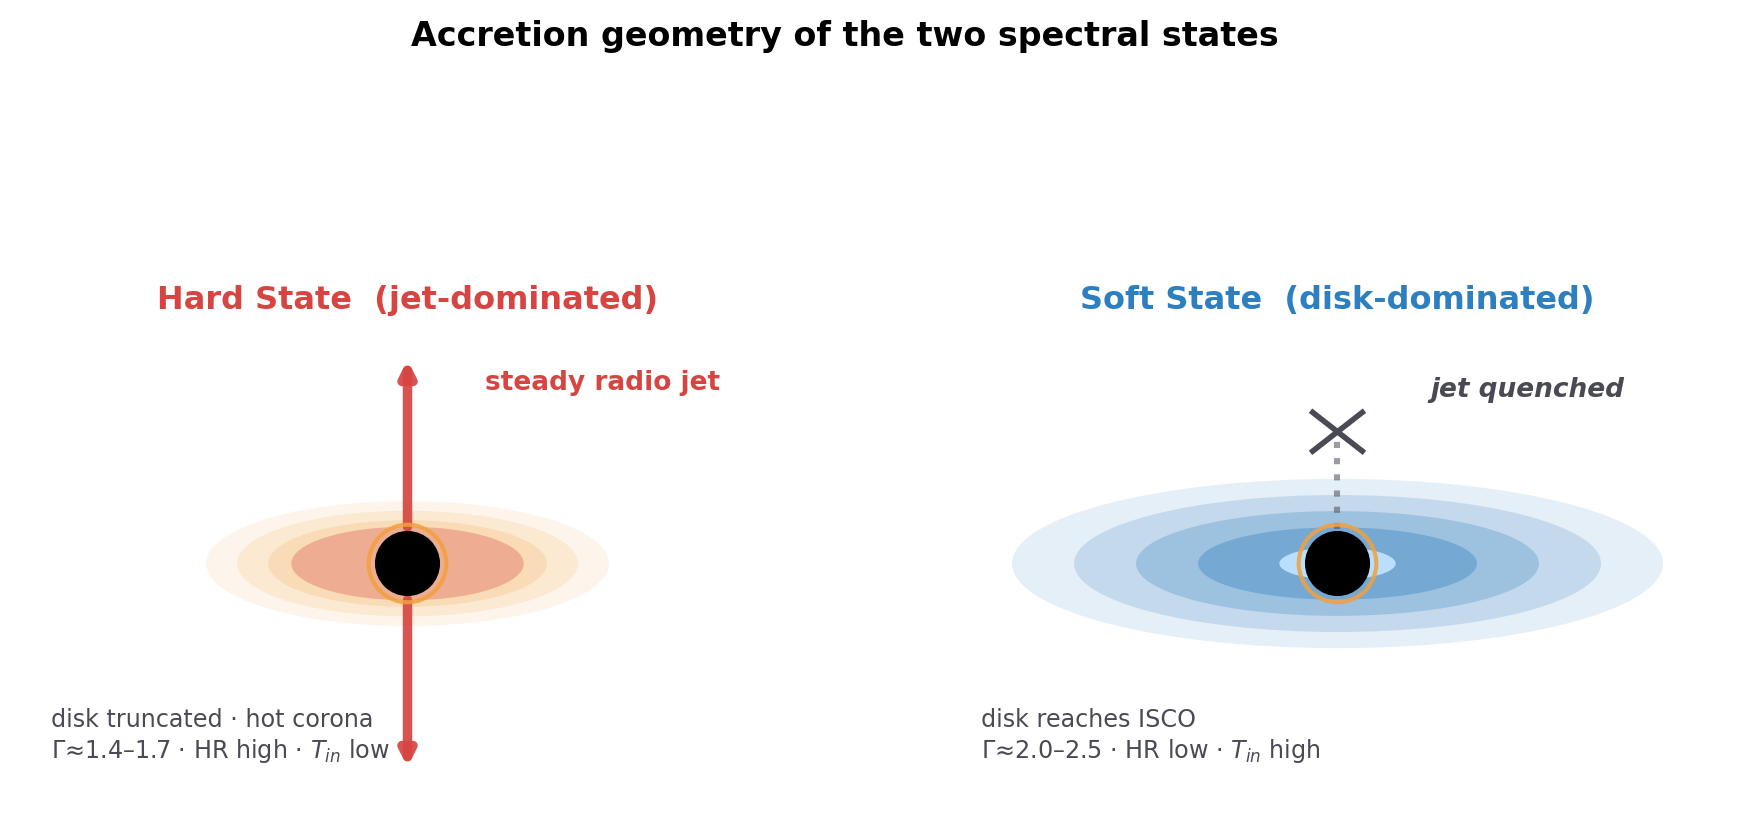
\includegraphics[width=\textwidth]{figs/fig01_accretion_states.png}
\caption{Accretion geometry of the two spectral states. In the Hard State the disk is truncated and replaced inward by a hot corona, with a steady radio jet. In the Soft State the disk extends to the innermost stable circular orbit and the jet is quenched.}
    \label{fig:section-c-1}
\end{figure}

Figure~\ref{fig:section-c-1} compares the two accretion states. In the Hard State,
the inner disk is truncated and replaced by a hot corona, while a steady radio jet
is present. In the Soft State, the disk extends to the innermost stable circular
orbit and the radio jet is quenched.



\begin{figure}[htbp]
    \centering
    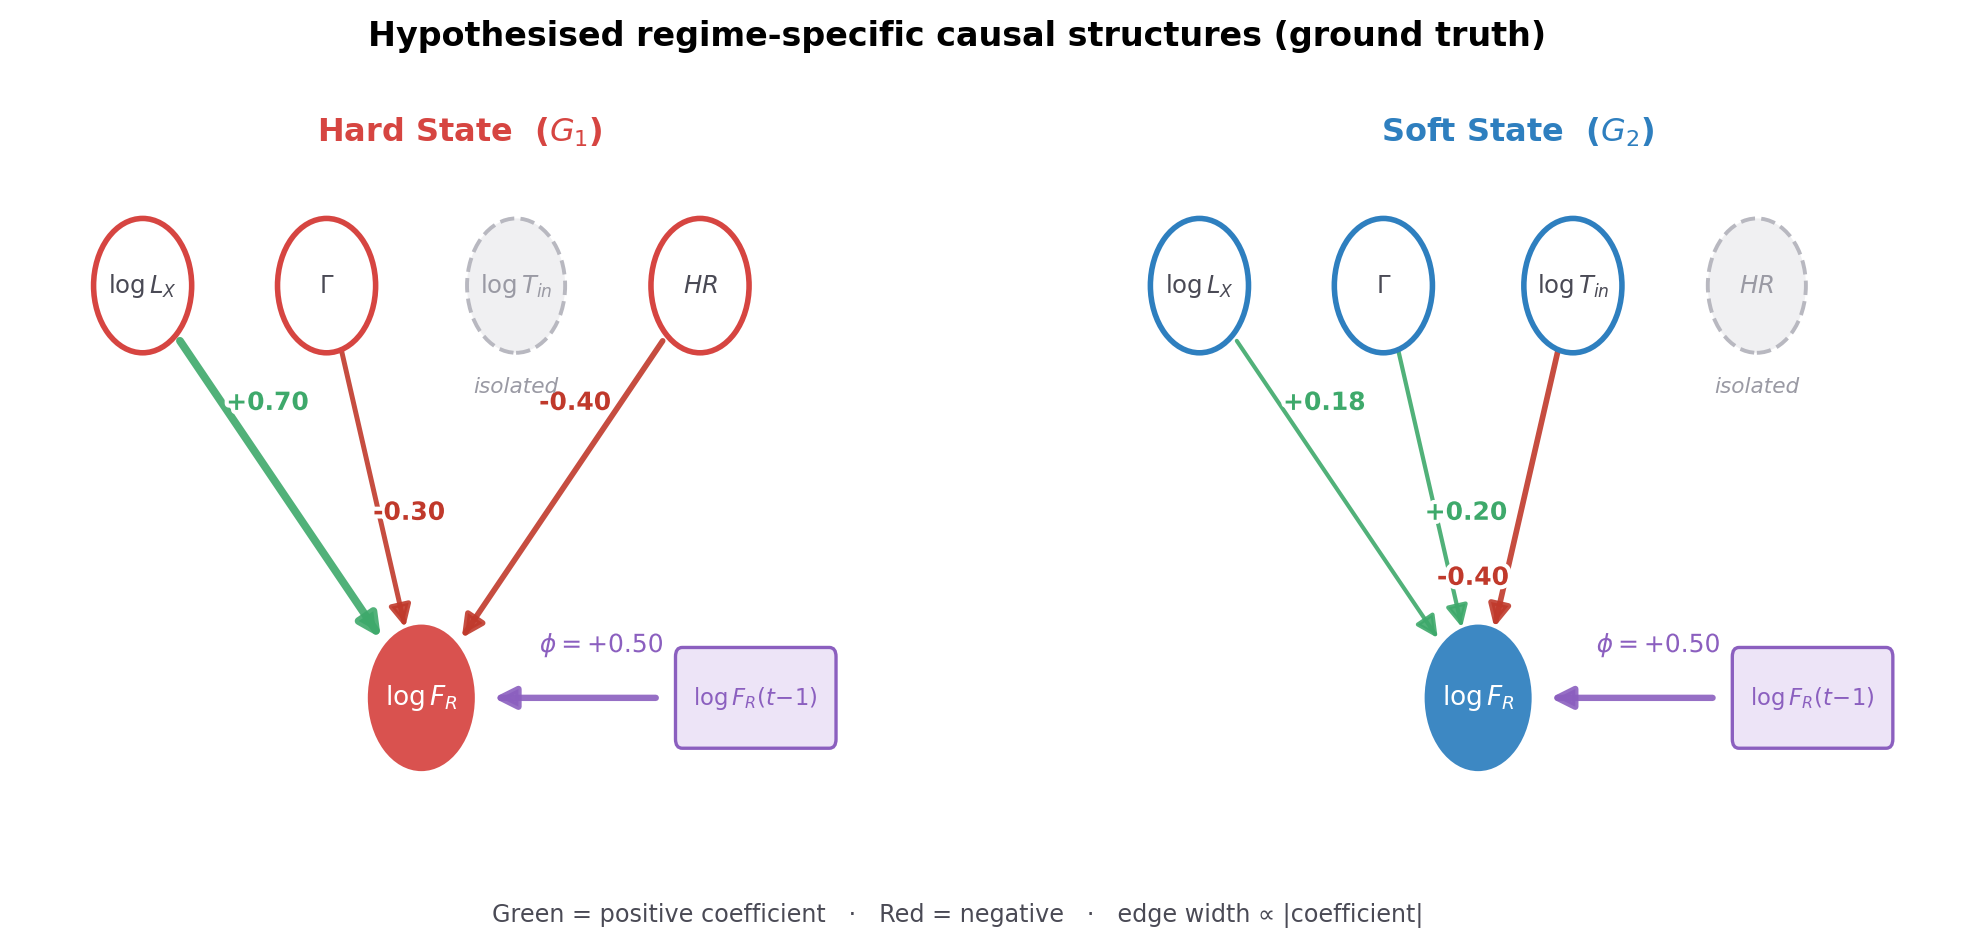
\includegraphics[width=\textwidth]{figs/fig02_ground_truth_dags.png}
\caption{Hypothesised causal structures for the hard and soft accretion states.}
    \label{fig:section-c-2}
\end{figure}

Figure~\ref{fig:section-c-2} shows the hypothesised causal structures for the two
states. The variables that influence radio luminosity differ between the Hard and
Soft States, and the isolated variable also changes. These regime-specific
structures motivate the graph-recovery stage of LIRA.

\begin{figure}[htbp]
    \centering
    \resizebox{\textwidth}{!}{%
    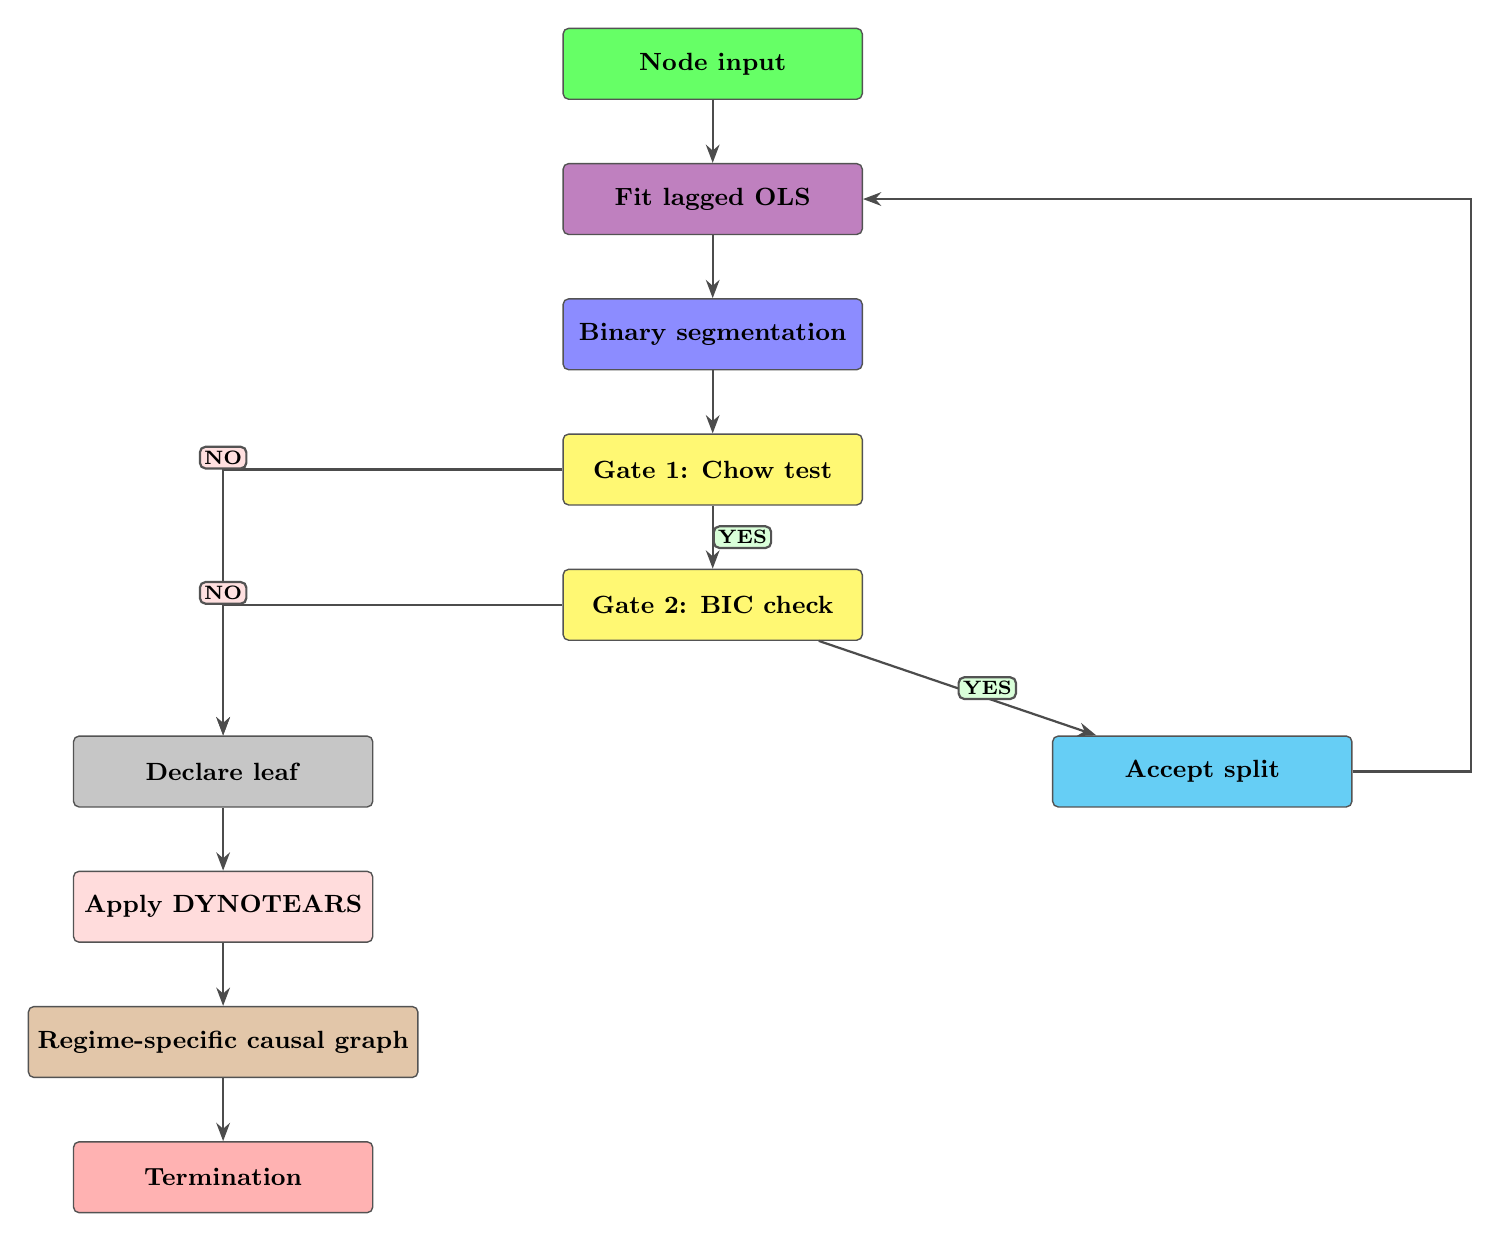
\begin{tikzpicture}[
        >=Stealth,
        node distance=8mm and 18mm,
        every node/.style={font=\small, align=center},
        process/.style={draw=gray!65!black, line width=0.5pt, rounded corners=2pt, minimum width=38mm, minimum height=9mm, text=black, fill=cyan!60},
        stage/.style={draw=gray!65!black, line width=0.5pt, rounded corners=2pt, minimum width=38mm, minimum height=9mm, text=black, fill=violet!50},
        gate/.style={draw=gray!65!black, line width=0.5pt, rounded corners=2pt, minimum width=38mm, minimum height=9mm, text=black, fill=orange!55},
        leaf/.style={draw=gray!65!black, line width=0.5pt, rounded corners=2pt, minimum width=38mm, minimum height=9mm, text=black, fill=gray!50},
        output/.style={draw=gray!65!black, line width=0.5pt, rounded corners=2pt, minimum width=38mm, minimum height=9mm, text=black, fill=teal!55},
        inputbox/.style={process, fill=green!60},
        olsbox/.style={stage, fill=violet!50},
        binbox/.style={stage, fill=blue!45},
        chowbox/.style={gate, fill=yellow!55},
        bicbox/.style={gate, fill=yellow!55},
        leafbox/.style={leaf, fill=gray!45},
        dynobox/.style={output, fill=pink!55},
        graphbox/.style={output, fill=brown!45},
        acceptbox/.style={process, fill=cyan!60},
        terminationbox/.style={leaf, fill=red!30},
        yes/.style={draw=gray!65!black, fill=green!15, rounded corners=2pt, inner sep=1.5pt, text=black, font=\bfseries\scriptsize},
        no/.style={draw=gray!65!black, fill=red!12, rounded corners=2pt, inner sep=1.5pt, text=black, font=\bfseries\scriptsize},
        line/.style={->, thick, draw=gray!60!black}
    ]
        \node[inputbox] (input) {\textbf{Node input}};
        \node[olsbox, below=of input] (ols) {\textbf{Fit lagged OLS}};
        \node[binbox, below=of ols] (binseg) {\textbf{Binary segmentation}};
        \node[chowbox, below=of binseg] (chow) {\textbf{Gate 1: Chow test}};
        \node[bicbox, below=of chow] (bic) {\textbf{Gate 2: BIC check}};
        \node[leafbox, below left=12mm and 24mm of bic] (leafnode) {\textbf{Declare leaf}};
        \node[dynobox, below=of leafnode] (dyno) {\textbf{Apply DYNOTEARS}};
        \node[graphbox, below=of dyno] (graph) {\textbf{Regime-specific causal graph}};
        \node[terminationbox, below=of graph] (stop) {\textbf{Termination}};
        \node[acceptbox, below right=12mm and 24mm of bic] (accept) {\textbf{Accept split}};

        \draw[line] (input) -- (ols);
        \draw[line] (ols) -- (binseg);
        \draw[line] (binseg) -- (chow);
        \draw[line] (chow) -- node[right, yes] {YES} (bic);
        \draw[line] (chow) -| node[above, no] {NO} (leafnode);
        \draw[line] (bic) -| node[above, no] {NO} (leafnode);
        \draw[line] (bic) -- node[right, yes] {YES} (accept);
        \draw[line] (leafnode) -- (dyno);
        \draw[line] (dyno) -- (graph);
        \draw[line] (graph) -- (stop);
        \draw[line] (accept.east) -- ++(15mm,0) |- (ols.east);
    \end{tikzpicture}%
    }
    \caption{Step-by-step recursive framework for temporal regime discovery and dynamic causal graph recovery, combining lagged OLS estimation, Binary Segmentation, Chow and BIC gates, and DYNOTEARS.}
    \label{fig:pipeline}
\end{figure}

Figure~\ref{fig:pipeline} summarises the complete procedure. The method fits a
lagged OLS model, searches for a candidate boundary with binary segmentation, and
passes it through the Chow and BIC gates. Accepted splits are processed recursively.
When a leaf is reached, DYNOTEARS estimates the regime-specific causal graph. The
validation results for this process are presented in Chapter 5.

\section{Log-space linearisation}

The Fundamental Plane of Black Hole Activity expresses radio luminosity as a power law
in X-ray luminosity and black hole mass, as shown in Equation~\eqref{eq:ch4-1}:

\begin{equation}
    \label{eq:ch4-1}
L_R \propto L_X^{\xi_X} \cdot M_{BH}^{\xi_M}
\end{equation}

Taking logarithms converts Equation~\eqref{eq:ch4-1} into coefficients and addition:

\begin{equation}
    \label{eq:ch4-2}
\log L_R = \xi_X \log L_X + \xi_M \log M_{BH} + c
\end{equation}

Equation~\eqref{eq:ch4-2} is linear. This form is required by OLS, the Chow test,
the $F$-distribution derivation, BIC, and the linear DYNOTEARS model. In raw flux
space the relationships would remain multiplicative, so these linear-model results
would not apply. The reasoning is summarised in Equation~\eqref{eq:ch4-3}:

\begin{equation}
    \label{eq:ch4-3}
\text{accretion physics} \Rightarrow \text{power laws} \Rightarrow \text{log-linearity} \Rightarrow \text{OLS valid} \Rightarrow \text{Chow and BIC valid}
\end{equation}

The log transform is derived from the physical scaling law rather than chosen only as
a generic preprocessing step.

Table~\ref{tab:ch4-variables} gives the transformation used for each variable.



\begin{table}[htbp]
    \centering
    \small
    \caption{Variable set and transformation}
    \label{tab:ch4-variables}
    \begin{tabularx}{\textwidth}{|>{\raggedright\arraybackslash}p{1.3cm}|>{\raggedright\arraybackslash}p{2.6cm}|>{\raggedright\arraybackslash}p{1.9cm}|>{\raggedright\arraybackslash}X|}
        \hline
        Symbol & Quantity & Transform & Justification \\ \hline
        $F_R$ & radio luminosity & $\log$ & Luminosity. Power-law coupled and spans orders of magnitude. \\ \hline
        $L_X$ & X-ray luminosity & $\log$ & Luminosity. Power-law coupled and spans orders of magnitude. \\ \hline
        $T_{in}$ & inner disk temperature & $\log$ & multicolor disk models give power-law scaling with luminosity \\ \hline
        $\Gamma$ & photon index & none & already a dimensionless spectral slope, itself an exponent. Range $\approx 1.4$--$2.5$ \\ \hline
        $HR$ & hardness ratio & none & already a bounded dimensionless ratio. The same argument applies as for $\Gamma$. \\ \hline
\end{tabularx}
\end{table}

The dimensionless, bounded variables $\Gamma$ and $HR$ are left unchanged. They do
not require logarithmic compression, and the power-law argument does not apply to
them.

The spectral-state diagnostics used by the model are summarised in Table~\ref{tab:ch4-states}.


\section{The structural model}


\subsection{Absorption of black hole mass}

Equation~\eqref{eq:ch4-2} contains $\log M_{BH}$. For a single accreting source observed over
time, $M_{BH}$ is constant: it cannot vary between time steps. A constant term in a
regression equation is absorbed entirely by the intercept, as shown in Equation~\eqref{eq:ch4-4}:

\begin{equation}
    \label{eq:ch4-4}
\xi_M \log M_{BH} \;\longrightarrow\; \text{folded into } w_0
\end{equation}

so mass is absorbed into the intercept. This is the correct treatment of a
within-source constant. LIRA's coefficients therefore describe variation within one
source and are not directly comparable to the cross-source Fundamental Plane
exponents.


\subsection{Spectral-state variables}

The model needs time-varying quantities to distinguish physical states. The standard
spectral-state diagnostics provide these variables, as summarised in
Table~\ref{tab:ch4-states}.



\begin{table}[htbp]
    \centering
    \small
    \caption{Spectral-state diagnostics and their regime dependence}
    \label{tab:ch4-states}
    \begin{tabularx}{\textwidth}{|>{\raggedright\arraybackslash}p{1.8cm}|>{\raggedright\arraybackslash}p{2.5cm}|>{\raggedright\arraybackslash}p{2.5cm}|>{\raggedright\arraybackslash}X|}
        \hline
        Variable & Hard State & Soft State & Physical quantity indexed \\ \hline
        $\log L_X$ & lower & higher & accretion rate \\ \hline
        $\Gamma$ & flat, $\approx1.4$--$1.7$ & steep, $\approx2.0$--$2.5$ & Comptonisation vs. disk emission \\ \hline
        $\log T_{in}$ & lower (disk truncated) & higher (disk at ISCO) & disk inner radius / geometry \\ \hline
        $HR$ & high & low & spectral hardness \\ \hline
\end{tabularx}
\end{table}

These variables do not replace mass. They capture temporal state variation within one
source, which the cross-source Fundamental Plane does not represent. The resulting
static specification is given in Equation~\eqref{eq:ch4-5}:

\begin{equation}
    \label{eq:ch4-5}
\log F_R(t) = w_0 + w_1 \log L_X(t) + w_2 \Gamma(t) + w_3 \log T_{in}(t) + w_4 HR(t) + \varepsilon(t)
\end{equation}


\subsection{The autoregressive extension}

The static specification in Equation~\eqref{eq:ch4-5} would require i.i.d. errors,
which real accretion time series do not satisfy. Time series show memory from viscous
timescales, turbulence, propagating
fluctuations, and persistent jets. The main consequences are:

\begin{enumerate}
    \item OLS coefficient estimates remain unbiased.
    \item Standard errors are underestimated.
    \item \textbf{The Chow $F$-statistic breaks.} Its denominator assumes i.i.d. residuals. Under
autocorrelation the denominator is artificially small, the $F$-statistic
artificially large, and the procedure detects regime boundaries that do not exist.
\end{enumerate}

The third consequence is the most important: unmodelled autocorrelation can create
false regime boundaries. We address it by adding the first-order autoregressive term
in Equation~\eqref{eq:ch4-6}:

\begin{equation}
    \label{eq:ch4-6}
\log F_R(t) = w_0 + w_1 \log L_X(t) + w_2 \Gamma(t) + w_3 \log T_{in}(t) + w_4 HR(t) + \phi \log F_R(t-1) + \varepsilon(t)
\end{equation}

Here, $\phi$ absorbs the temporal dependence, making $\varepsilon(t)$ approximately
i.i.d. and restoring the test assumptions. Section~5.2 verifies this result.

The coefficient $\phi$ measures temporal persistence and can be compared across
regimes (Section~5.4).

Lag one is used as the minimum sufficient choice. Additional lags increase $q$, reduce
the residual degrees of freedom, and make smaller regime segments harder to estimate.
If residual autocorrelation remains, Newey--West standard errors provide a robustness
check.


\subsection{Choice of estimator}

\textbf{Regularised regression is excluded.} Ridge and Lasso add penalties
($\lambda\|\beta\|_2^2$ and $\lambda\|\beta\|_1$ respectively) that shrink coefficients
toward zero, biasing the estimates. Since the Chow test consists entirely of comparing
the coefficient vectors of two groups, shrinking both corrupts the comparison: the test
would partly detect differences induced by the penalty rather than by genuine mechanism
change. Stage 1 therefore requires unbiased estimates and must not regularise.

This is deliberately in contrast with Stage 2, where DYNOTEARS does employ an $L_1$
penalty. The two stages answer different questions. Stage 2 asks \textit{which edges exist},
for which sparsity is essential. Stage 1 asks \textit{whether two coefficient vectors are
equal}, for which bias is fatal.

\textbf{Polynomial terms are excluded.} The log-linear form is derived from power-law
physics (Section~4.2). Terms such as $(\log L_X)^2$ have no physical motivation, invite
overfitting, and violate the assumption of common functional form across groups
required by the $F$-statistic derivation.


\subsection{Design matrix}

The design matrix has shape $(n-1, 6)$, the first observation being unavailable as a
response because it has no lag. Equations~\eqref{eq:ch4-7} and~\eqref{eq:ch4-8}
show the design matrix and response vector:

\begin{equation}
    \label{eq:ch4-7}
X_{lag} = \begin{bmatrix}
1 & \log L_X(2) & \Gamma(2) & \log T_{in}(2) & HR(2) & \log F_R(1) \\
1 & \log L_X(3) & \Gamma(3) & \log T_{in}(3) & HR(3) & \log F_R(2) \\
\vdots & \vdots & \vdots & \vdots & \vdots & \vdots \\
1 & \log L_X(n) & \Gamma(n) & \log T_{in}(n) & HR(n) & \log F_R(n-1)
\end{bmatrix}
\end{equation}

\begin{equation}
    \label{eq:ch4-8}
Y = [\log F_R(2), \log F_R(3), \ldots, \log F_R(n)]^\top
\end{equation}

With the OLS solution given by the normal equation in Equation~\eqref{eq:ch4-9},
Equation~\eqref{eq:ch4-10} gives the residuals and residual sum of squares:

\begin{equation}
    \label{eq:ch4-9}
\hat{w} = (X_{lag}^\top X_{lag})^{-1} X_{lag}^\top Y, \qquad \hat{w} = [w_0, w_1, w_2, w_3, w_4, \phi]^\top
\end{equation}

\begin{equation}
    \label{eq:ch4-10}
\hat{\varepsilon} = Y - X_{lag}\hat{w}, \qquad RSS_{global} = \hat{\varepsilon}^\top \hat{\varepsilon}
\end{equation}

$RSS_{global}$ measures how well a \textbf{single} causal model fits the entire series and
serves as the baseline against which all partitions are compared.


\section{Gate 1: the lagged Chow test}


\subsection{Hypothesis and intuition}

\begin{equation}
    \label{eq:ch4-11}
H_0 : w_A = w_B
\end{equation}

Equation~\eqref{eq:ch4-11} is the null hypothesis. Rejecting it indicates that the
mechanism differs between the two groups. If the two states follow different laws,
separate models should have lower residual error than one pooled model. The test
determines whether this reduction is statistically significant.

Note that $w$ includes the intercept $w_0$. This has a direct consequence for the
design of the validation data, addressed in Section~5.1.


\subsection{Construction}

For a candidate split, let $A$ denote observations before and $B$ after. Separate fits
are given in Equations~\eqref{eq:ch4-12} and~\eqref{eq:ch4-13}:

\begin{equation}
    \label{eq:ch4-12}
\hat{w}_A = (X_A^\top X_A)^{-1} X_A^\top Y_A, \quad RSS_A = \|Y_A - X_A\hat{w}_A\|^2
\end{equation}
\begin{equation}
    \label{eq:ch4-13}
\hat{w}_B = (X_B^\top X_B)^{-1} X_B^\top Y_B, \quad RSS_B = \|Y_B - X_B\hat{w}_B\|^2
\end{equation}

Equation~\eqref{eq:ch4-14} gives the Chow statistic. The cost of pooling is $RSS_{global} - (RSS_A + RSS_B)$, which is near zero when both
groups share one causal law. Normalising by the within-group variance
$\hat\sigma^2 = (RSS_A + RSS_B)/(n-2q)$ yields the lagged Chow statistic:

\begin{equation}
    \label{eq:ch4-14}
F_{lag} = \frac{\big[RSS_{global} - (RSS_A + RSS_B)\big] / q}{(RSS_A + RSS_B)/(n - 2q)}
\end{equation}

The numerator is divided by $q$ because the split adds $q$ parameters. The denominator
has $n-2q$ degrees of freedom, the residual degrees of freedom after fitting two
models.


\subsection{Degrees of freedom}

The value $q = 6$ follows directly from the structural model of Section~4.3 and is not a
tuning parameter: the intercept $w_0$ (which absorbs $\xi_M \log M_{BH}$), the four
spectral-state coefficients $w_1$--$w_4$, and the autoregressive coefficient $\phi$.


\subsection{Distribution}

Under $H_0$ and Gaussian i.i.d. residuals, Equation~\eqref{eq:ch4-15} gives the numerator and denominator distributions:
independent chi-square variates,

\begin{equation}
    \label{eq:ch4-15}
\big[RSS_{global} - (RSS_A + RSS_B)\big]/\sigma^2 \sim \chi^2(q), \qquad (RSS_A + RSS_B)/\sigma^2 \sim \chi^2(n-2q)
\end{equation}

and the ratio of two independent chi-square variables each divided by its degrees of
freedom is $F$-distributed by definition, as shown in Equation~\eqref{eq:ch4-16}:

\begin{equation}
    \label{eq:ch4-16}
F_{lag} \sim F(q,\; n-2q) \quad \text{under } H_0
\end{equation}

\begin{equation}
    \label{eq:ch4-17}
p = P\big(F(q, n-2q) > F_{obs}\big) = 1 - \mathrm{CDF}_F(F_{obs}, q, n-2q)
\end{equation}

$H_0$ is rejected at $\alpha=0.05$. The test requires Gaussian residuals, which also
constrains the downstream causal-discovery model. This issue is discussed in
Section~4.6.


\section{Locating the boundary and Gate 2}


\subsection{Binary segmentation}

The test of Section~4.4 requires a split point to be supplied. Since the boundary location is
unknown, the statistic is evaluated at every admissible index and maximised, as shown
in Equation~\eqref{eq:ch4-18}:

\begin{equation}
    \label{eq:ch4-18}
\tau^* = \arg\max_{\tau} F_{lag}\big(A(\tau), B(\tau)\big)
\end{equation}

where $A(\tau) = \{2,\ldots,\tau\}$ and $B(\tau) = \{\tau+1,\ldots,n\}$. The maximising
index is the location at which the data most strongly prefers two models to one.

Exhaustive search over all multi-way partitions is intractable. Binary segmentation
is therefore used as a greedy divide-and-conquer method: it finds the best split and
then repeats the search within each child segment. This procedure is not guaranteed
to find the global optimum.

A minimum segment size of $2q=12$ is enforced. Smaller segments do not support
stable matrix inversion, and the $F$-test degrees of freedom approach zero. Segments
near this minimum can still produce noisy coefficients and unreliable graphs.

\textbf{Note on splitting variable.} Splitting is performed on the time index only.
Feature-threshold splitting of the form $(j^*, \tau^*)$ is not employed, as the
autoregressive term of (4.5) presupposes temporal contiguity within each segment.


\subsection{Derivation of the BIC criterion}

A significant $F$-statistic shows that a difference is detectable, but a greedy search
can find apparently favourable splits caused by noise. Without a stopping rule, the
algorithm would continue splitting until the segments became too small. BIC provides
the required complexity penalty.

\textbf{Step A: the Gaussian likelihood.} For $Y = Xw + \varepsilon$ with
$\varepsilon_t \sim N(0,\sigma^2)$ i.i.d., Equation~\eqref{eq:ch4-19} gives the Gaussian likelihood.

\begin{equation}
    \label{eq:ch4-19}
\log P(Y \mid w, \sigma^2, M) = -\frac{n}{2}\log(2\pi) - \frac{n}{2}\log(\sigma^2) - \frac{RSS}{2\sigma^2}
\end{equation}

\textbf{Step B: substitution of the MLE.} With $\hat\sigma^2 = RSS/n$, Equation~\eqref{eq:ch4-20} gives the likelihood at the MLE.

\begin{equation}
    \label{eq:ch4-20}
\log P(Y \mid \hat{w}, \hat\sigma^2, M) = -\frac{n}{2}\log(2\pi) - \frac{n}{2}\log\!\left(\frac{RSS}{n}\right) - \frac{n}{2}
\end{equation}

The terms $-\frac{n}{2}\log(2\pi)$ and $-\frac{n}{2}$ do not depend on the model and
cancel in any comparison, leaving the simplified likelihood in Equation~\eqref{eq:ch4-21}:

\begin{equation}
    \label{eq:ch4-21}
\log P \approx -\frac{n}{2}\log\!\left(\frac{RSS}{n}\right)
\end{equation}

\textbf{Step C: the criterion.} Schwarz's criterion, obtained from the Laplace
approximation to the marginal likelihood, is $BIC = -2\log P(Y \mid \hat\theta, M) + k\log(n)$
for $k$ free parameters. Substituting Equation~\eqref{eq:ch4-19}, we obtain the BIC
given in Equation~\eqref{eq:ch4-22}:

\begin{equation}
    \label{eq:ch4-22}
BIC = n\log\!\left(\frac{RSS}{n}\right) + k\log(n)
\end{equation}

\textbf{Step D: the one-model case.} For a single global model over $n$ observations with
$q = 6$ parameters, Equation~\eqref{eq:ch4-23} gives the one-model BIC:

\begin{equation}
    \label{eq:ch4-23}
BIC_1 = n\log\!\left(\frac{RSS_{global}}{n}\right) + q\log(n)
\end{equation}

\textbf{Step E: the two-model case.} For disjoint segments the combined log-likelihood is
the sum of the two independent log-likelihoods, each with its own MLE
$\hat\sigma_A^2 = RSS_A/n_A$ and $\hat\sigma_B^2 = RSS_B/n_B$. With $2q$ total free
parameters, as shown in Equation~\eqref{eq:ch4-24}:

\begin{equation}
    \label{eq:ch4-24}
BIC_2 = n_A\log\!\left(\frac{RSS_A}{n_A}\right) + n_B\log\!\left(\frac{RSS_B}{n_B}\right) + 2q\log(n)
\end{equation}

\textbf{Step F: the choice of $\log(n)$.} The penalty uses the total sample size $n$,
following the Bai--Perron convention for structural-break models. Using $n_A$ and
$n_B$ separately would make small segments cheaper and encourage over-partitioning.
Using total $n$ keeps the two scores on a common scale.

\textbf{Step G: decision rule.} A split is accepted if and only if $BIC_2 < BIC_1$.
Subtracting the penalty of Equation~\eqref{eq:ch4-23} from the penalty of
Equation~\eqref{eq:ch4-24} gives the net penalty
increase from splitting, as shown in Equation~\eqref{eq:ch4-25}:

\begin{equation}
    \label{eq:ch4-25}
2q\log(n) - q\log(n) = q\log(n)
\end{equation}

which is the exact price, in units of $-2\log$-likelihood, of admitting one additional
regime.


\subsection{Why BIC rather than AIC}

AIC imposes a penalty of $2k$, constant in sample size. BIC imposes $k\log(n)$, which
grows with the data. Table~\ref{tab:ch4-bic} gives the comparison at $k = q = 6$.



\begin{table}[htbp]
    \centering
    \small
    \caption{Complexity penalty comparison}
    \label{tab:ch4-bic}
    \begin{tabularx}{\textwidth}{|X|X|X|X|}
        \hline
        $n$ & AIC penalty & BIC penalty & Ratio \\ \hline
        800 & 12 & 40.1 & 3.3$\times$ \\ \hline
        5,000 & 12 & 51.1 & 4.3$\times$ \\ \hline
        10,000 & 12 & 55.3 & 4.6$\times$ \\ \hline
\end{tabularx}
\end{table}

For regime discovery, a false split can corrupt both resulting graphs, while a missed
split gives a conservative pooled model. BIC's stronger, sample-size-dependent
penalty is therefore appropriate for this task.


\subsection{The two-gate design}

The two criteria serve different purposes. The Chow test asks whether the difference
is statistically detectable. BIC asks whether the improvement justifies the added
complexity. A split can pass the first test and fail the second, as shown in Section~5.3.


\section{Identifiability}

For a linear structural equation model with Gaussian noise, edge direction within a
\textit{chain} ($X \to Y \to Z$) or \textit{fork} ($X \leftarrow Y \to Z$) is not identifiable from
observational data: for any true $X \to Y$ there exists a reversed model with rescaled
coefficient and noise variance inducing an identical joint distribution. No algorithm
can recover the direction, as the information is absent from the data.

A \textit{collider}, several mutually independent parents converging on a common effect, is
the exception. Collider orientation is recoverable from conditional-independence
structure alone, irrespective of noise distribution. This is the v-structure argument
on which constraint-based discovery rests generally.

\textbf{The model of Section~4.3 is a collider.} $\log L_X$, $\Gamma$, $\log T_{in}$, and $HR$ are
specified as parents of $\log F_R$ and not of one another. Direction is therefore
identifiable here for structural reasons rather than incidentally.

This has a consequence for possible extensions that is worth stating explicitly.
Suppose the model were enriched with causal chains among the spectral variables. Those
edges would be chains and forks, and recovering their orientation would require
non-Gaussian innovations together with a LiNGAM-family estimator. However, the
$F$-distribution result (4.14) requires Gaussian residuals for the numerator and
denominator to be independent chi-square variates, and the BIC derivation (4.17)--(4.20)
begins from the Gaussian log-likelihood. Adopting non-Gaussian noise to secure
identifiability in Stage 2 would therefore weaken the distributional derivations
underpinning both gates of Stage 1. The collider specification avoids this tension:
Gaussian noise is retained, (4.14) and (4.20) hold exactly as derived, and Stage 2
orientations remain identifiable. The restriction to a collider structure is thus a
defended design decision rather than a simplifying convenience.


\section{Stage 2: regime-specific causal graphs}

Each leaf is a temporally contiguous segment treated as a stable causal regime, and
DYNOTEARS is applied independently within each. Two matrices are estimated
simultaneously: $W$, in which $W_{ij} \neq 0$ indicates that variable $j$ affects
variable $i$ within the same time step, and $A$, in which $A_{ij} \neq 0$ indicates
that variable $j$ at $t-1$ affects variable $i$ at $t$. Acyclicity of the
contemporaneous graph is enforced by the smooth algebraic constraint
$\mathrm{tr}(e^{W \circ W}) - d = 0$, replacing combinatorial search with
gradient-based optimisation.

DYNOTEARS is preferred to the PC algorithm on two grounds. The first, noted in Section~2.1.6,
is that PC returns a skeleton and partial orientation without edge weights and
requires a number of conditional independence tests that grows sharply once lagged
variables are admitted. The second is decisive in practice: the Fisher-Z test assumes
independent samples, an assumption violated outright by consecutive observations of an
autoregressive process with $\phi \approx 0.9$. Applied to such data, the test's null
distribution is misspecified, and in preliminary experiments this produced orientations
into variables that have no parents by construction.

Two implementation requirements are recorded. First, variables must be standardised
within each leaf before fitting, as the DYNOTEARS objective and its sparsity threshold
are scale-sensitive. Without standardisation, edges belonging to lower-variance
variables are systematically underweighted and may be eliminated by the $L_1$ penalty.
Second, the terminality of $F_R$ must be encoded as explicit per-edge exclusions
forbidding $F_R$ at any lag from being a parent of $L_X$, $\Gamma$, $T_{in}$, or $HR$.
A blanket node-level prohibition also suppresses the edge $F_R(t-1) \to F_R(t)$, which
the model of (4.5) explicitly requires.


\section{Stage 3: causal effect estimation and validation}

Stages 1 and 2 yield a graph. Stage 3 quantifies the effects it encodes and assesses
how far those quantities should be trusted.

For each discovered parent of $F_R$ within each regime, the causal effect is estimated
by backdoor adjustment, conditioning on the remaining parents. Unpenalised regression
is used here, for the reason given in Section~4.3.4: with the structure already determined,
regularisation contributes only bias. The lag term $\log F_R(t-1)$ must be included in
every adjustment set, since the predictors are autocorrelated with their own past and
$F_R(t-1)$ lies downstream of that past. Omitting it allows a predictor to absorb part
of the lag term's effect.

Three refutation procedures are applied. A \textbf{random common cause} test injects an
irrelevant synthetic covariate, under which a valid estimate should be unchanged. A
\textbf{placebo treatment} test replaces the treatment with a permuted version, under which
the estimated effect should collapse to zero. This is the diagnostic that would expose
a procedure generating effects from noise. A \textbf{data subset} test re-estimates on an
80% subsample, guarding against dependence on particular observations.

\textbf{Sensitivity analysis} is then applied in the partial-$R^2$ parameterisation of
Cinelli and Hazlett, which reports a \textit{robustness value}: the minimum proportion of
residual variance in both treatment and outcome that an unobserved confounder would
need to explain in order to reduce the estimate to zero. Unobserved confounding cannot
be excluded from observational data, and Section~1.6 identifies it as a principal challenge
for this application. The robustness value converts that acknowledged limitation into
a stated numerical threshold against which domain knowledge can be brought to bear.

Finally, \textbf{graph falsification} tests whether the conditional-independence
implications of the entire recovered DAG are consistent with the data, by comparing
its violation count against randomly permuted graphs. Where the preceding tests
validate individual effects conditional on the graph, this interrogates the graph
itself.


\section{Parameter summary}

The complete parameter specification is given in Table~\ref{tab:ch4-parameters}.



\begin{table}[htbp]
    \centering
    \small
    \caption{Complete parameter specification}
    \label{tab:ch4-parameters}
    \begin{tabularx}{\textwidth}{|>{\raggedright\arraybackslash}X|>{\raggedright\arraybackslash}p{1.7cm}|>{\raggedright\arraybackslash}X|}
        \hline
        Parameter & Value & Determined by \\ \hline
        Variables log-transformed & $F_R, L_X, T_{in}$ & power-law scaling (Section~4.2) \\ \hline
        Variables untransformed & $\Gamma, HR$ & dimensionless, bounded range (Section~4.2) \\ \hline
        $q$ (parameters per model) & 6 & structural model: $w_0$, $w_1$--$w_4$, $\phi$ (Section~4.4.3) \\ \hline
        Chow numerator d.f. & $q = 6$ & parameters gained by splitting (Section~4.4.2) \\ \hline
        Chow denominator d.f. & $n - 2q$ & residual d.f. after two fits (Section~4.4.2) \\ \hline
        $\alpha$ & 0.05 & conventional; asymmetric error cost handled by Gate 2 \\ \hline
        $BIC$ penalty, one model & $q\log(n)$ & Schwarz criterion (Section~4.5.2) \\ \hline
        $BIC$ penalty, two models & $2q\log(n)$ & Bai--Perron convention, total $n$ (Section~4.5.2) \\ \hline
        Net cost of a split & $q\log(n)$ & Eq. (4.25) \\ \hline
        Lag order & 1 & minimum sufficient; higher orders raise $q$ (Section~4.3.3) \\ \hline
        Minimum segment size & $2q = 12$ & invertibility and $F$-test stability (Section~4.5.1) \\ \hline
        Splitting variable & time index & required by AR term (Section~4.5.1) \\ \hline
\end{tabularx}
\end{table}




% \chapter{Result Analysis}
% This thesis introduced LIRA (Latent Invariant Regime Analysis), a framework for
finding hidden causal regimes in black hole accretion time series. The method uses
the power-law physics of the Fundamental Plane and models the observations with a
log-linear structural equation. Black hole mass is included in the intercept, while
four spectral-state variables describe changes over time. LIRA finds regime
boundaries through recursive partitioning, a lagged Chow $F$-test, and the Bayesian
Information Criterion. DYNOTEARS then estimates the causal graph inside each
regime. The results are checked with refutation tests, sensitivity analysis, and graph
falsification.

The synthetic experiments produced strong results. LIRA found the true boundary
within four observations out of ten thousand. It also found the correct number of
regimes. It recovered the structural coefficients to within $0.017$ of their true
values.

The isolated variable in each regime was identified correctly. Clustering methods
that ignored causal structure performed poorly. A pooled model also gave an averaged
structure that matched neither regime.

The two-gate design was useful. The Chow test alone would have created extra splits.
The BIC gate rejected those unnecessary splits.

Several limitations remain. The most important one is that every result in this
thesis was obtained from synthetic data. The synthetic experiments show that LIRA
works when the data follow the assumptions it was designed for. They do not show that
it works on real black hole observations.

Real X-ray light curves contain gaps. They also contain instrumental artefacts and
sources of variability that the generator does not reproduce. The pipeline may behave
differently once it is applied to them.

The simulation also uses the same linear and piecewise-stationary structure that LIRA
assumes during recovery. The tests are therefore favourable to the method by
construction.

Beyond the data itself, the model assumes linear and piecewise-stationary
relationships. Real accretion systems may change in nonlinear and continuous ways
instead. The identifiability result also depends on the collider structure used in
this thesis. It may not hold for a model with causal chains between the spectral
variables.

The sensitivity analysis showed that the weaker coupling in the Soft State supports
weaker causal claims than the Hard State.

The next step is to move from synthetic validation to real data. This is the single
most important piece of future work. Real observations are the only way to test
whether the regimes LIRA finds correspond to physical accretion states. They also
show whether the regimes are artefacts of the simulation.

The recommended sequence mirrors the phase structure used in this thesis. LIRA should
first be applied to well-monitored sources with dense coverage. GRS 1915+105 and
Cygnus X-1 are good candidates. Their known state transitions provide an external
check on the discovered boundaries.

The analysis should then be extended to the WATCHDOG catalogue. It offers a broader
sample of sources and longer baselines.

In both cases, the discovered regimes should be compared against independently
identified Hard and Soft States. The recovered causal graphs should be checked
against the physical expectations discussed in Chapter 2.

Any disagreement between the synthetic and real-data results should be treated as a
finding in its own right. It would locate exactly where the simulation assumptions
break down.

Other useful steps include testing nonlinear mechanisms. LIRA can also be compared
with CASTOR on the same benchmark. Future work can also allow causal structure to
change gradually rather than at fixed boundaries.

Together, these extensions would address the gap between the controlled synthetic
validation reported here and the noisier, less predictable behaviour of real
accretion systems.


\chapter{Experimental Validation}


\section{Experimental design}


\subsection{Rationale for synthetic validation}

Real observations do not provide ground truth for regime boundaries or causal graphs.
This prevents direct measurement of recovery accuracy. Synthetic structural causal
models have known graphs and coefficients, so every output can be evaluated: regimes
with the Adjusted Rand Index, graphs against the generating DAG, effects against the
generating coefficients, and persistence against the true $\phi$.


\subsection{Generating process}

Two regimes of 5,000 observations are generated in temporal order and concatenated
without shuffling. The four spectral-state variables follow independent,
mean-reverting first-order autoregressive processes:

Equation~\eqref{eq:ch5-1} defines the mean-reverting process:
\begin{equation}
    \label{eq:ch5-1}
X(t) = \mu_X + \varphi\big(X(t-1) - \mu_X\big) + \epsilon_X(t), \qquad \varphi = 0.90
\end{equation}

with $\epsilon_X(t) \sim N(0, 0.10^2)$ for all four variables. The mean-reverting
form preserves the chosen mean from the first step. It therefore avoids the decay of
initial values and removes the need for a burn-in period.

The target variable is generated by Equation~\eqref{eq:ch5-2}:

\begin{equation}
    \label{eq:ch5-2}
\log F_R(t) = \mu_F + \phi\big(\log F_R(t-1) - \mu_F\big) + \sum_{v} \beta_v^{(z)}\big(X_v(t) - \mu_v\big) + \epsilon_F(t)
\end{equation}

with $\phi = 0.50$. The predictors are centred and $F_R$ is mean-reverting. Thus,
$\mathrm{E}[\log F_R] = \mu_F$ for any coefficient vector, so both regimes have the
same means.


\subsection{Why equal means are necessary for a valid test}

Equal means are necessary for a meaningful test. The Chow null hypothesis in
Equation~\eqref{eq:ch4-11} compares the full coefficient vectors, including the
intercept $w_0$. A mean shift would change the intercept and could cause rejection
without any change in the causal slopes. Structure-blind clustering would also benefit
from that level shift, making the baseline comparison uninformative.

With equal means, the regimes differ only in which variable has a non-zero coefficient
on $\log F_R$. A rejection can therefore reflect a mechanism change. Table~\ref{tab:ch5-distribution}
confirms the construction.



\begin{table}[htbp]
    \centering
    \small
    \caption{Distributional summary of the generated data}
    \label{tab:ch5-distribution}
    \begin{tabularx}{\textwidth}{|>{\raggedright\arraybackslash}X|>{\raggedright\arraybackslash}X|>{\raggedright\arraybackslash}X|>{\raggedright\arraybackslash}X|>{\raggedright\arraybackslash}X|}
        \hline
        Variable & Hard mean & Soft mean & Hard s.d. & Soft s.d. \\ \hline
        $\log L_X$ & 37.4931 & 37.4756 & 0.2332 & 0.2290 \\ \hline
        $\Gamma$ & 1.6124 & 1.5909 & 0.2347 & 0.2174 \\ \hline
        $\log T_{in}$ & 0.2934 & 0.3289 & 0.2188 & 0.2174 \\ \hline
        $HR$ & 0.7669 & 0.7320 & 0.2377 & 0.2297 \\ \hline
        $\log F_R$ & 27.9747 & 27.9595 & 0.3803 & 0.2289 \\ \hline
    \end{tabularx}
\end{table}

The means differ by less than 0.04 for every variable. The variance of $\log F_R$ is
still different (0.380 versus 0.229), because the Hard State has larger coefficient
magnitudes. This remaining difference is addressed in the baseline comparison.


\subsection{Ground-truth structures}



\begin{table}[htbp]
    \centering
    \small
    \caption{Generating coefficients}
    \label{tab:ch5-coefficients}
    \begin{tabularx}{\textwidth}{|>{\raggedright\arraybackslash}X|>{\raggedright\arraybackslash}X|>{\raggedright\arraybackslash}X|}
        \hline
        Coefficient & Hard State ($G_1$) & Soft State ($G_2$) \\ \hline
        $\beta_{L_X}$ & $+0.70$ & $+0.18$ \\ \hline
        $\beta_{\Gamma}$ & $-0.30$ & $+0.20$ \\ \hline
        $\beta_{T_{in}}$ & $0.00$ \textit{(isolated)} & $-0.40$ \\ \hline
        $\beta_{HR}$ & $-0.40$ & $0.00$ \textit{(isolated)} \\ \hline
        $\phi$ & $+0.50$ & $+0.50$ \\ \hline
    \end{tabularx}
\end{table}

The Hard State is interpreted as jet-dominated: radio emission is driven by X-ray
luminosity, photon index, and hardness ratio, while inner-disk temperature is isolated.
The Soft State is disk-dominated, with hardness ratio isolated instead.

The generating coefficients are listed in Table~\ref{tab:ch5-coefficients}.

The corresponding ground-truth causal structures are shown in Figure~\ref{fig:chapter5-2},
and the generated series and its true and discovered boundaries are shown in
Figure~\ref{fig:chapter5-3}.


\begin{figure}[htbp]
    \centering
    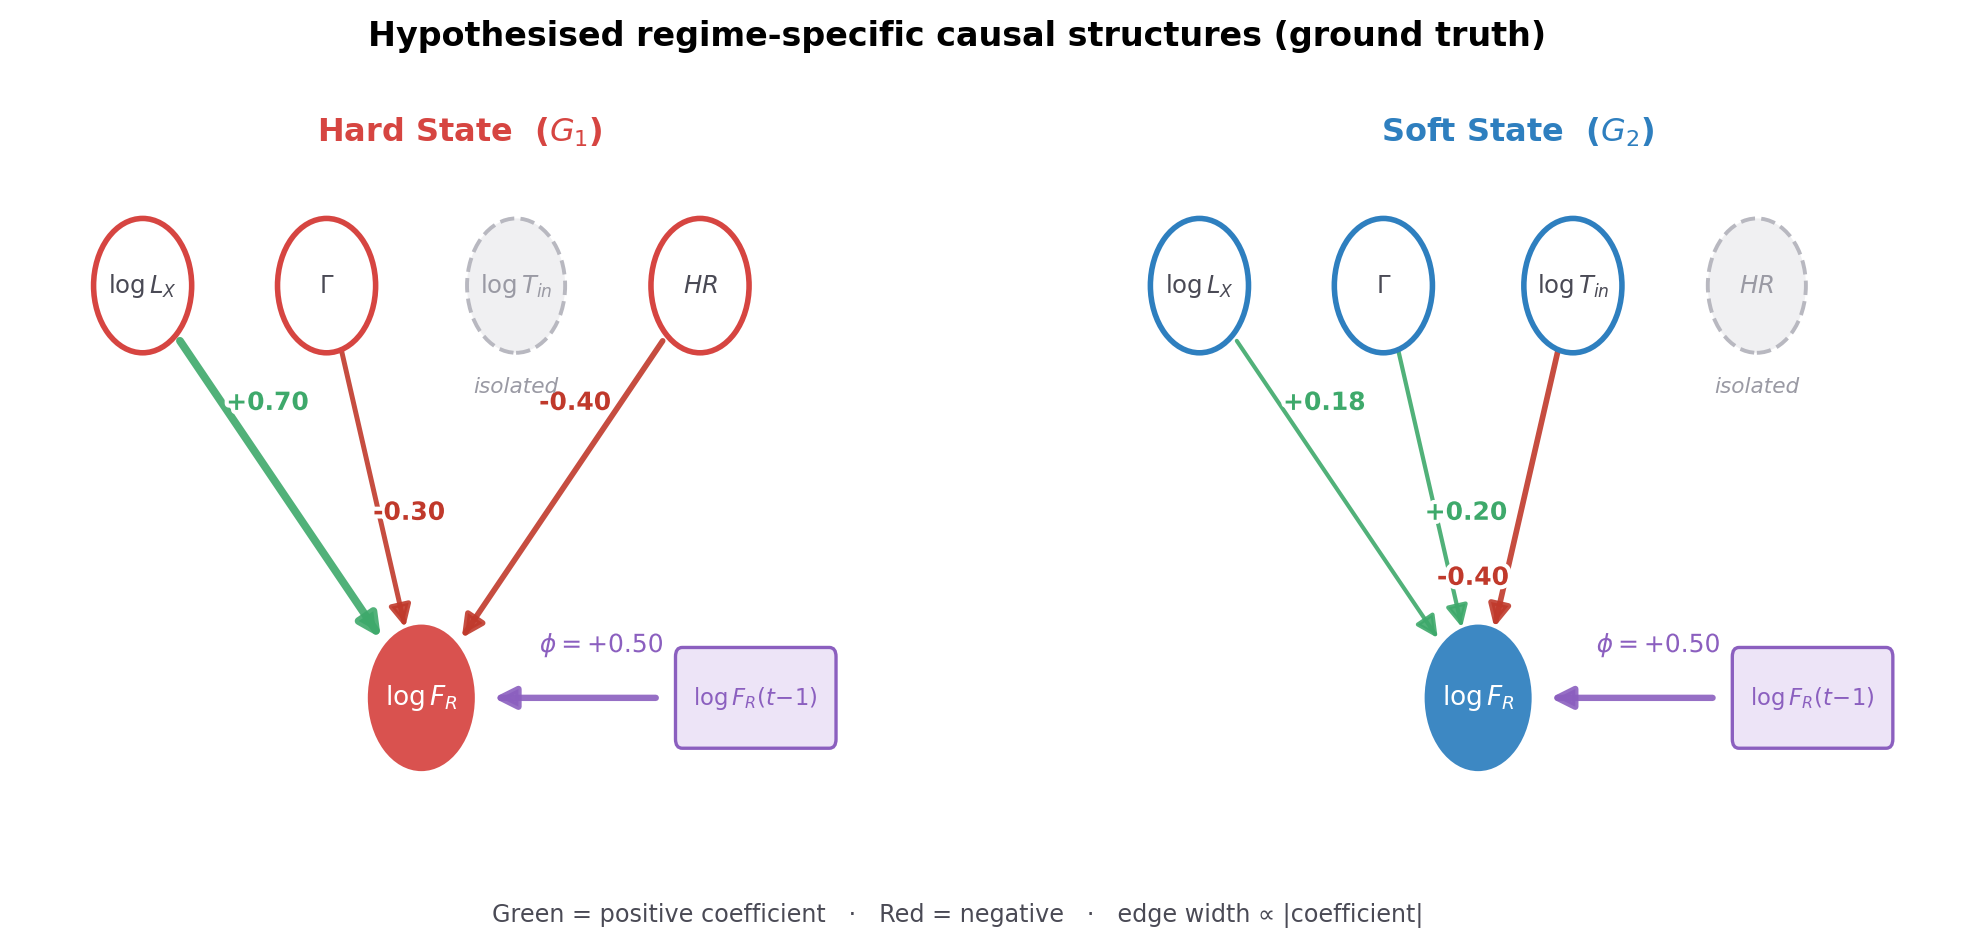
\includegraphics[width=\textwidth]{figs/fig02_ground_truth_dags.png}
\caption{Hypothesised regime-specific causal structures. Edge width is proportional to coefficient magnitude. The causally isolated variable in each regime is shown dashed.}
    \label{fig:chapter5-2}
\end{figure}

Figure~\ref{fig:chapter5-2} shows the causal structures used to generate the two
regimes. The Hard State contains edges from $L_X$, $\Gamma$, and $HR$ into $F_R$;
$T_{in}$ is isolated. In the Soft State, $T_{in}$ becomes a parent of $F_R$ and $HR$
is isolated. These mechanism changes are the target of regime discovery.


\begin{figure}[htbp]
    \centering
    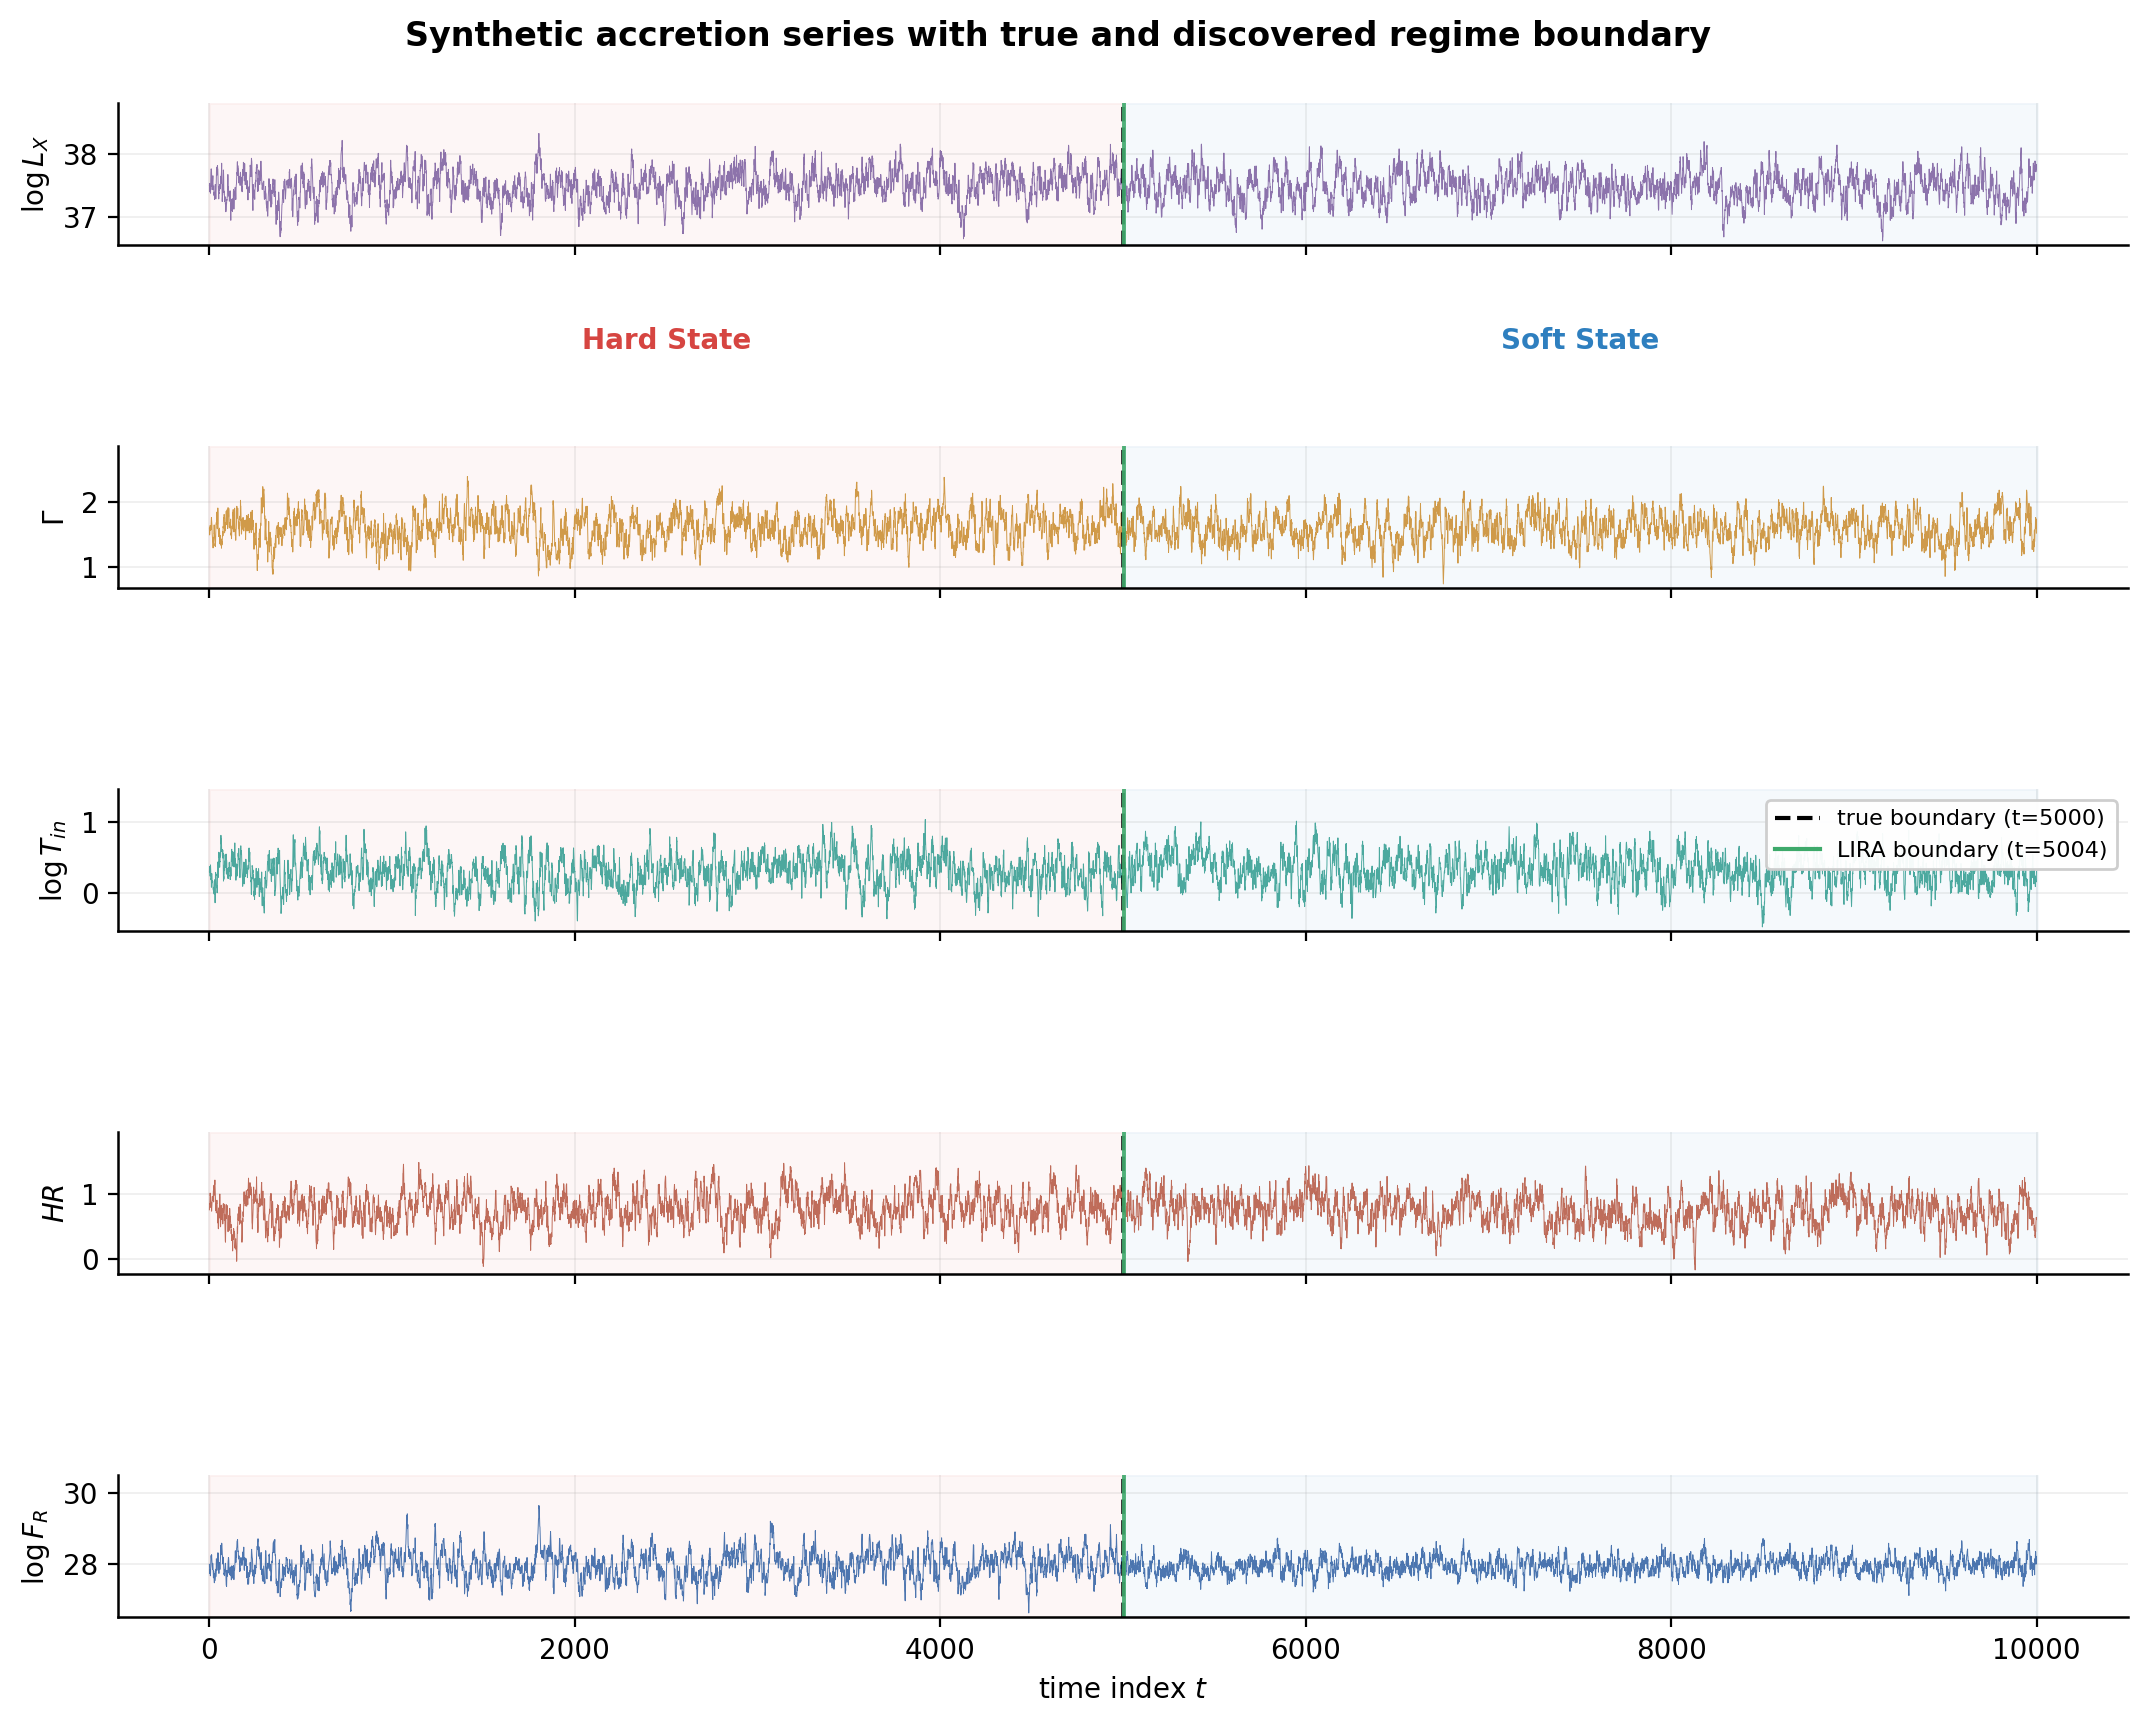
\includegraphics[width=\textwidth]{figs/fig03_timeseries.png}
\caption{The generated series with the true boundary (dashed) and the boundary discovered by LIRA (solid). No level shift is visible at the boundary in any variable, by construction.}
    \label{fig:chapter5-3}
\end{figure}

Figure~\ref{fig:chapter5-3} shows the generated series and the two boundaries. The
levels remain similar across the true boundary, so the regimes are not separated by
a simple mean shift. The recovered boundary is close to the generating boundary,
which supports the numerical localisation result in Section~5.3.1.


\section{Validation of the autoregressive extension}

Section~4.3.3 argues that the lag term is required for the Chow $F$ derivation to hold. This
is verified directly. Fitting the static specification in Equation~\eqref{eq:ch4-5} within the first regime
yields residuals with first-order autocorrelation $0.507$ and a Ljung--Box statistic at
10 lags of $1713.4$ ($p < 10^{-16}$), decisively rejecting independence. Fitting the
autoregressive specification in Equation~\eqref{eq:ch4-6} to the same data reduces the first-order residual
autocorrelation to $-0.011$, with a Ljung--Box statistic of $13.2$ ($p = 0.211$),
consistent with independence at any conventional level.

The residual-independence diagnostics are summarised in Table~\ref{tab:ch5-residuals}.



\begin{table}[htbp]
    \centering
    \small
    \caption{Residual independence diagnostics (Hard State segment)}
    \label{tab:ch5-residuals}
    \begin{tabularx}{\textwidth}{|>{\raggedright\arraybackslash}X|>{\raggedright\arraybackslash}X|>{\raggedright\arraybackslash}X|>{\raggedright\arraybackslash}X|>{\raggedright\arraybackslash}X|}
        \hline
        Specification & ACF(1) & Ljung--Box(10) & $p$ & Residuals i.i.d.? \\ \hline
        Static, Eq. (4.5) & $0.507$ & $1713.4$ & $<10^{-16}$ & rejected \\ \hline
        Autoregressive, Eq. (4.6) & $-0.011$ & $13.2$ & $0.211$ & not rejected \\ \hline
    \end{tabularx}
\end{table}

Table~\ref{tab:ch5-residuals} shows that the static model leaves strong residual
autocorrelation, while the AR(1) model produces residuals consistent with independence.
The corresponding autocorrelation plots are shown next.

\begin{figure}[htbp]
    \centering
    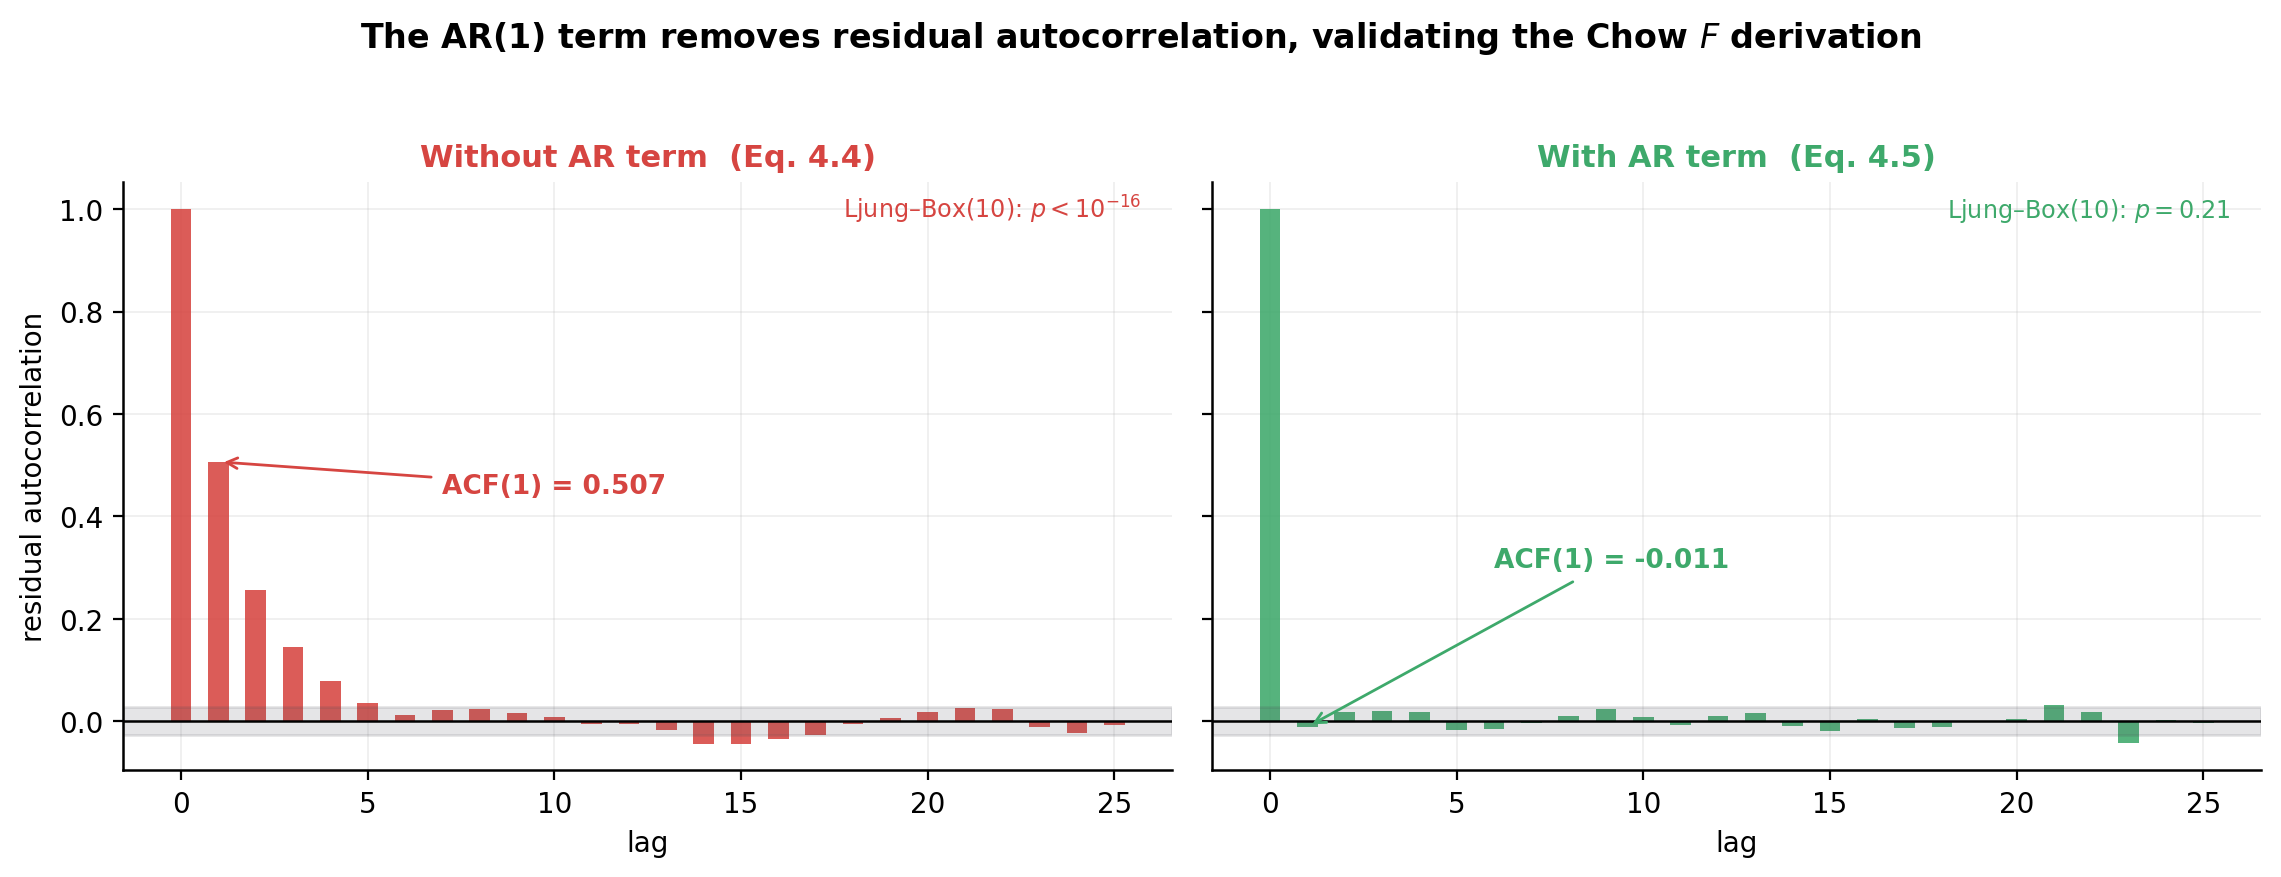
\includegraphics[width=\textwidth]{figs/fig06_residual_acf.png}
    \caption{Residual autocorrelation functions with and without the AR(1) term. Shaded band gives the 95\% interval under independence.}
    \label{fig:chapter5-6}
\end{figure}

The autoregressive specification therefore supports the distributional assumption in
Equation~\eqref{eq:ch4-15}, while the static specification does not. The lag term is
necessary, not merely beneficial.

Figure~\ref{fig:chapter5-6} shows the corresponding residual autocorrelation diagnostics.


\section{Regime discovery}


\subsection{Boundary localisation}

Figure~\ref{fig:chapter5-4} shows the lagged Chow statistic evaluated across all admissible split indices
at the root node. The statistic rises monotonically toward the true boundary and
attains its maximum of $F_{lag} = 963.4$ at $\tau^* = 5004$, against a true boundary at
$t = 5000$, a localisation error of four observations, or $0.04\%$ of the series
length. The associated $p$-value is below the limit of double-precision representation.


\begin{figure}[htbp]
    \centering
    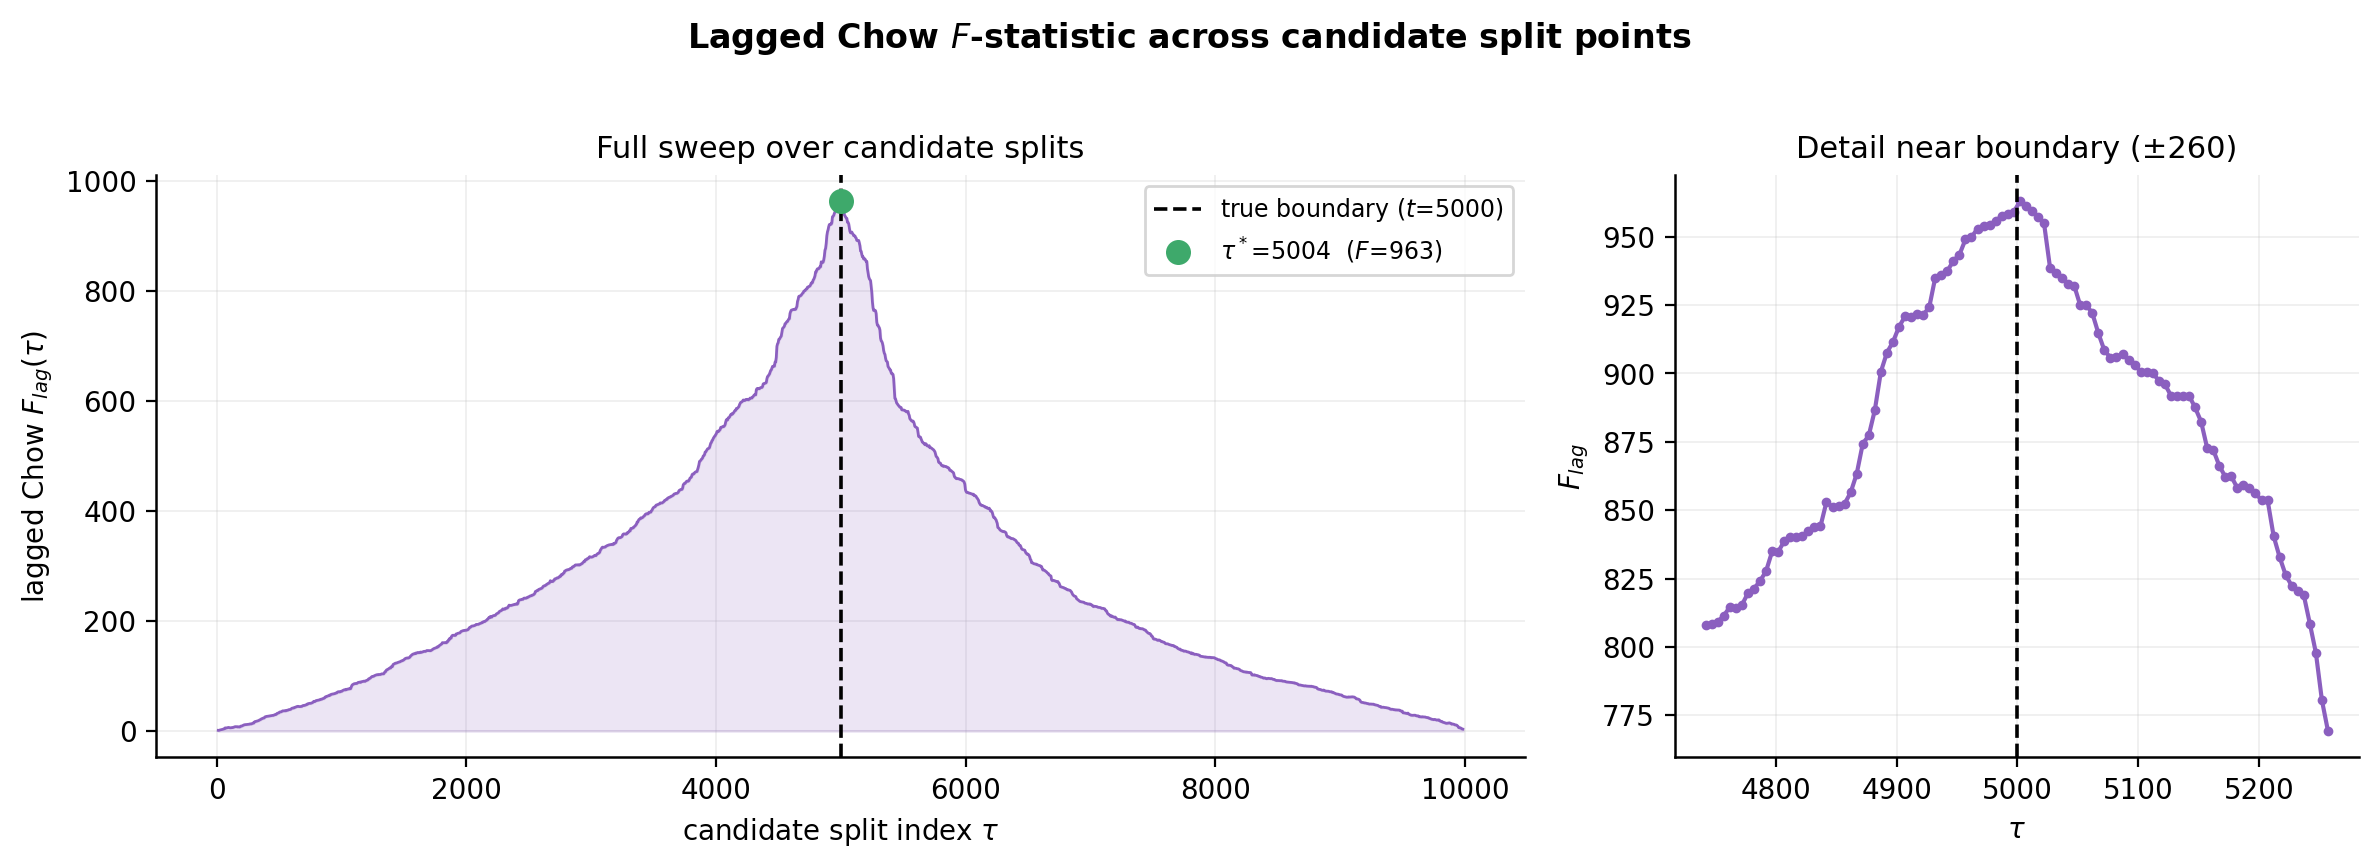
\includegraphics[width=\textwidth]{figs/fig04_chow_F_curve.png}
    \caption{Lagged Chow $F$-statistic across candidate split points, with detail near the boundary.}
    \label{fig:chapter5-4}
\end{figure}


\subsection{Operation of the two gates}

At the root node both gates are satisfied: $F_{lag} = 963.4$ with $p < 10^{-16}$, and
$BIC_1 = -41362$ against $BIC_2 = -45874$, so the split reduces BIC by $4512$ and is
accepted. Recursion then proceeds into each child.

At both child nodes the Chow test is significant: $F_{lag}=3.15$, $p=0.004$ on the
left and $F_{lag}=3.27$, $p=0.003$ on the right. A Chow-only procedure would have
created extra, spurious boundaries. BIC rejects both splits. The split increases BIC
by about $31$ in each child, so recursion stops with $K=2$.

The gate decisions at the root and child nodes are summarised in Table~\ref{tab:ch5-gates}.


\begin{table}[htbp]
    \centering
    \scriptsize
    \setlength{\tabcolsep}{3pt}
    \renewcommand{\arraystretch}{1.2}
    \caption{Gate evaluation at each recursion node}
    \label{tab:ch5-gates}
    \begin{tabularx}{\textwidth}{|>{\raggedright\arraybackslash}X|>{\raggedright\arraybackslash}X|>{\raggedright\arraybackslash}X|>{\raggedright\arraybackslash}X|>{\raggedright\arraybackslash}X|>{\raggedright\arraybackslash}X|>{\raggedright\arraybackslash}X|>{\raggedright\arraybackslash}X|>{\raggedright\arraybackslash}X|}
        \hline
        \makecell{Node} & $n$ & $F_{lag}$ & $p$ & \makecell{Gate\\1} & $BIC_1$ & $BIC_2$ & \makecell{Gate\\2} & \makecell{Outcome} \\ \hline
        root & 9,999 & 963.38 & $<10^{-16}$ & pass & $-41362$ & $-45874$ & pass & \textbf{split} at $t=5004$ \\ \hline
        left child & 5,003 & 3.15 & 0.0044 & pass & $-23026$ & $-22994$ & \textbf{fail} & leaf \\ \hline
        right child & 4,995 & 3.27 & 0.0033 & pass & $-22851$ & $-22820$ & \textbf{fail} & leaf \\ \hline
    \end{tabularx}
\end{table}

The child-node results show why both gates are needed. The Chow test detects a
possible difference, while BIC determines that the added complexity is not justified.

Figures~\ref{fig:chapter5-5} and~\ref{fig:chapter5-12} visualise the BIC decisions and
the realised recursion tree, respectively.

\begin{figure}[htbp]
    \centering
    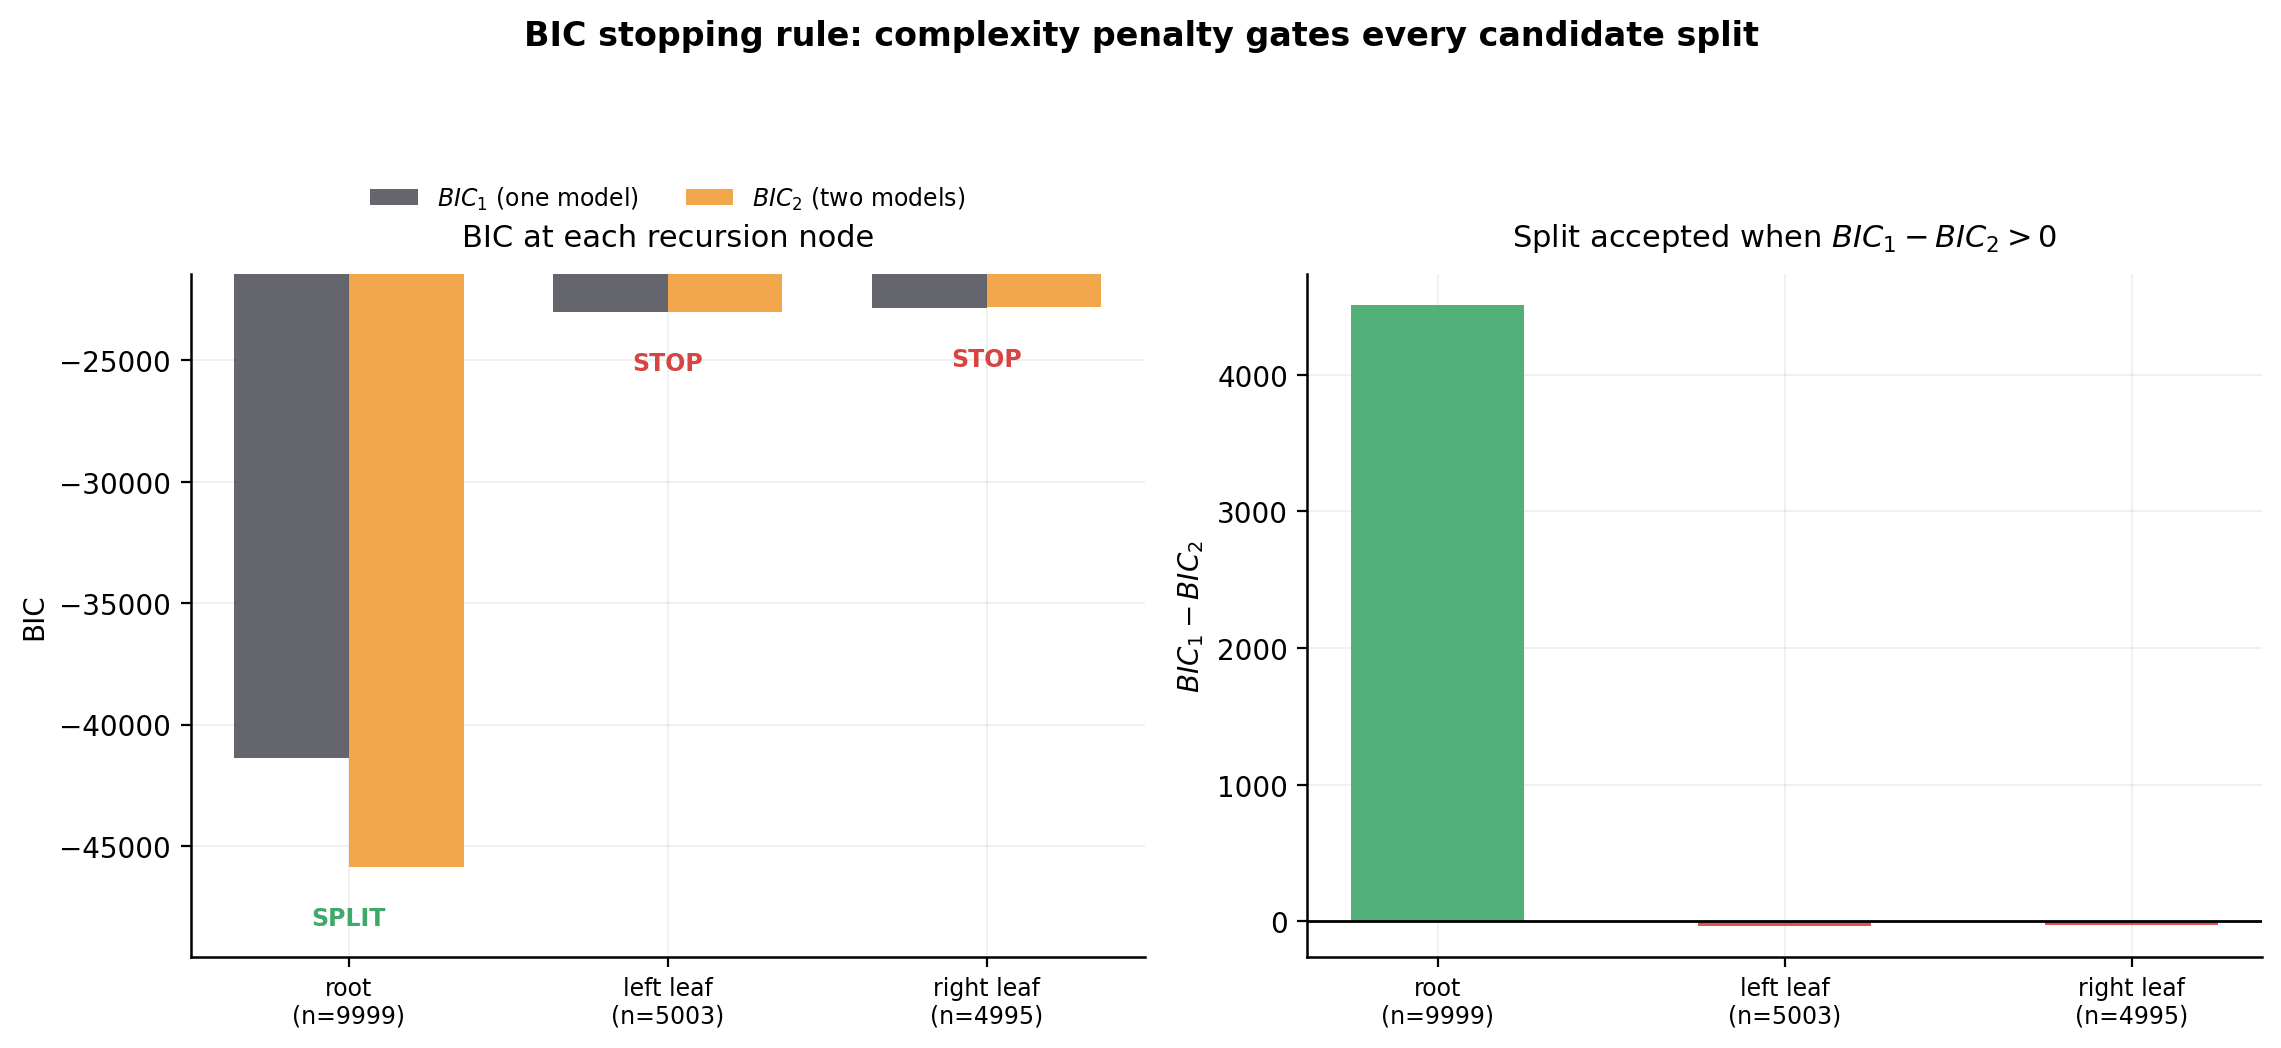
\includegraphics[width=\textwidth]{figs/fig05_bic_gate.png}
    \caption{BIC evaluation at each recursion node.}
    \label{fig:chapter5-5}
\end{figure}

Figure~\ref{fig:chapter5-5} gives the numerical BIC comparison. The root split has
the lower two-model BIC and is accepted, whereas both child splits have higher
two-model BIC values and are rejected.

\begin{figure}[htbp]
    \centering
    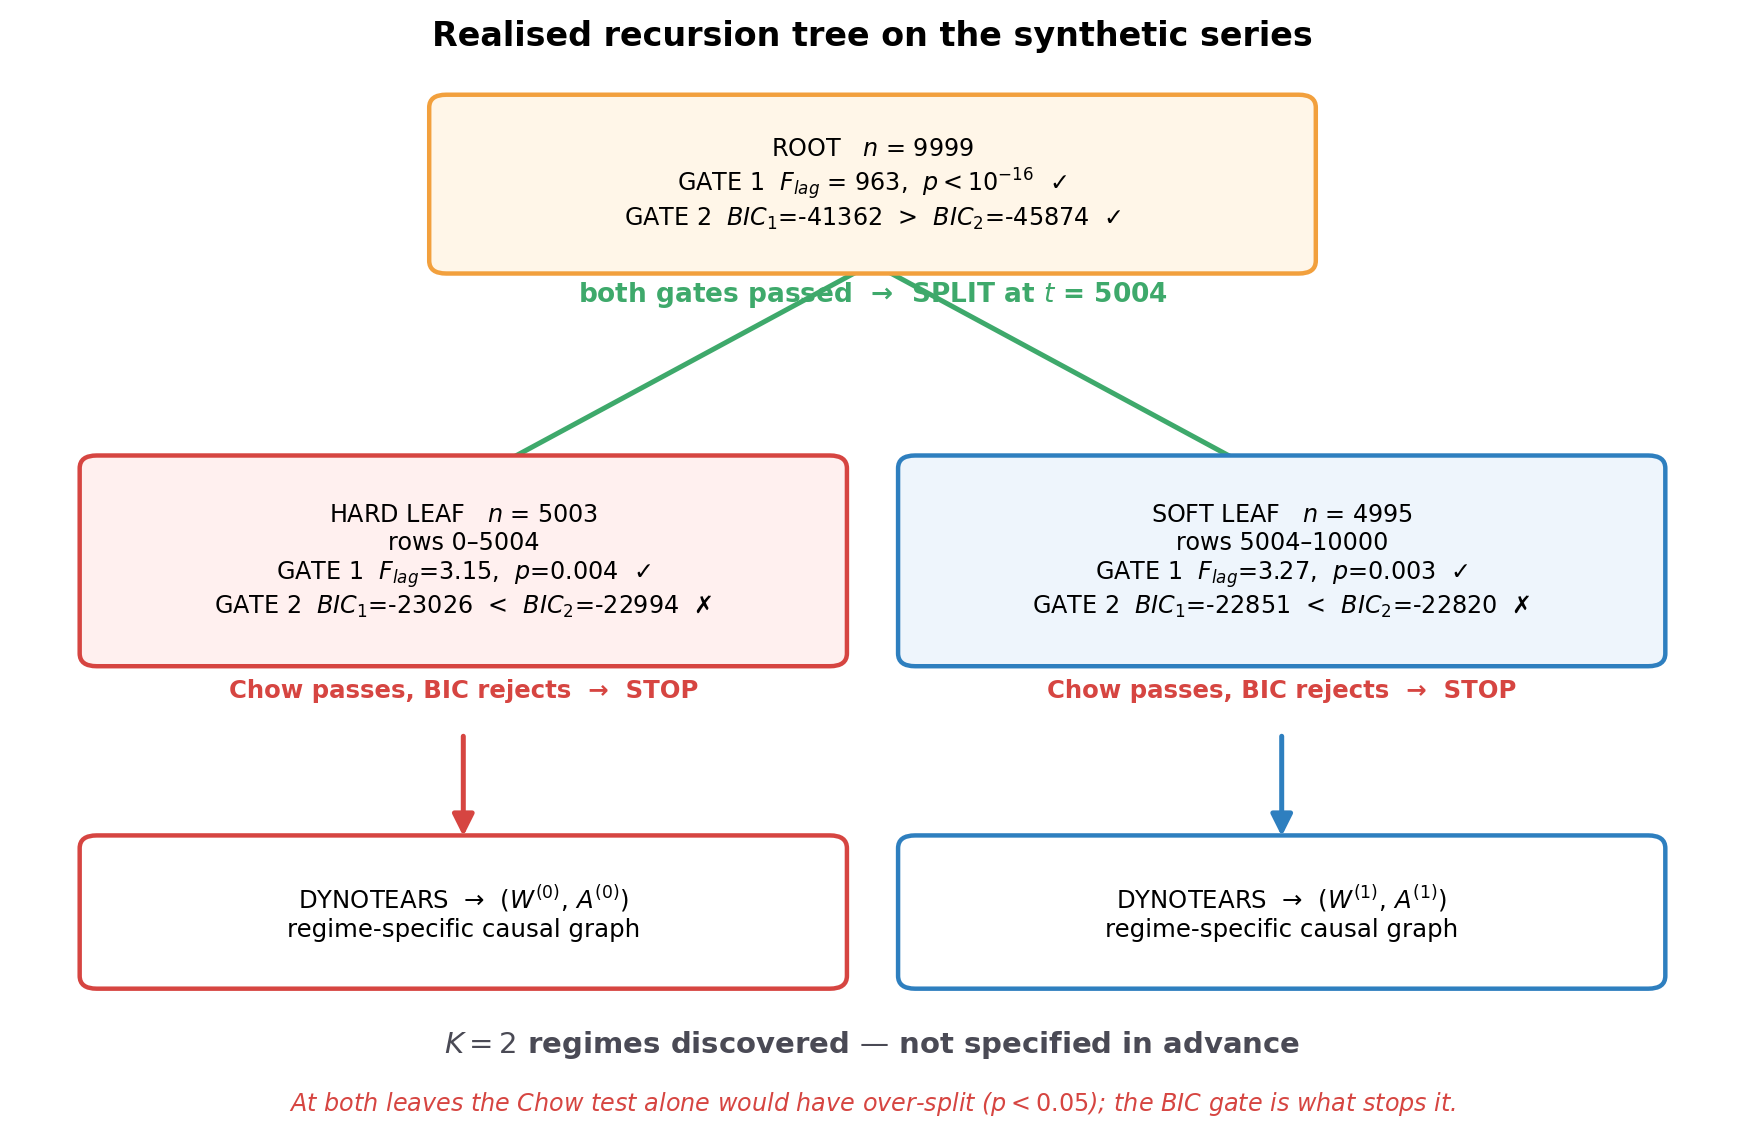
\includegraphics[width=\textwidth]{figs/fig12_recursion_tree.png}
    \caption{Realised recursion tree on the synthetic validation series.}
    \label{fig:chapter5-12}
\end{figure}

Figure~\ref{fig:chapter5-12} presents these decisions as a recursion tree. It shows
the accepted root split, the two terminal leaves, and the subsequent application of
DYNOTEARS. Together, the two figures explain how the final two-regime solution is
formed.


\subsection{Comparison against structure-blind baselines}

$K=2$ regimes are recovered with an Adjusted Rand Index of $0.9984$, without supplying
$K$ in advance. Table~\ref{tab:ch5-regime-recovery} compares this result with
$k$-means, which is given the correct value $K=2$. Even with this advantage,
feature-space clustering fails on three of the four variants.



\begin{table}[htbp]
    \centering
    \small
    \caption{Regime recovery accuracy}
    \label{tab:ch5-regime-recovery}
    \begin{tabularx}{\textwidth}{|>{\raggedright\arraybackslash}X|>{\raggedright\arraybackslash}X|>{\raggedright\arraybackslash}X|}
        \hline
        Method & Basis for grouping & ARI \\ \hline
        \textbf{LIRA (this work)} & causal mechanism invariance, $K$ not supplied & \textbf{0.9984} \\ \hline
        $k$-means, raw features ($K=2$ given) & feature-space proximity & 0.0011 \\ \hline
        $k$-means, standardised features ($K=2$ given) & feature-space proximity & 0.0009 \\ \hline
        $k$-means, rolling means ($K=2$ given, $w=200$) & local level & 0.0112 \\ \hline
        $k$-means, rolling s.d. of $\log F_R$ ($K=2$ given, $w=200$) & local dispersion & 0.5867 \\ \hline
    \end{tabularx}
\end{table}

The result supports the design in Section~5.1.3: the regimes are not separated well
by distributional similarity alone.

The rolling-standard-deviation baseline reaches $\mathrm{ARI}=0.587$. It is included
because the variance of $\log F_R$ differs between regimes. It recovers less than LIRA
and requires $K$ to be supplied in advance.

Figure~\ref{fig:chapter5-8} shows the regime-recovery comparison against the
structure-blind baselines.


\begin{figure}[htbp]
    \centering
    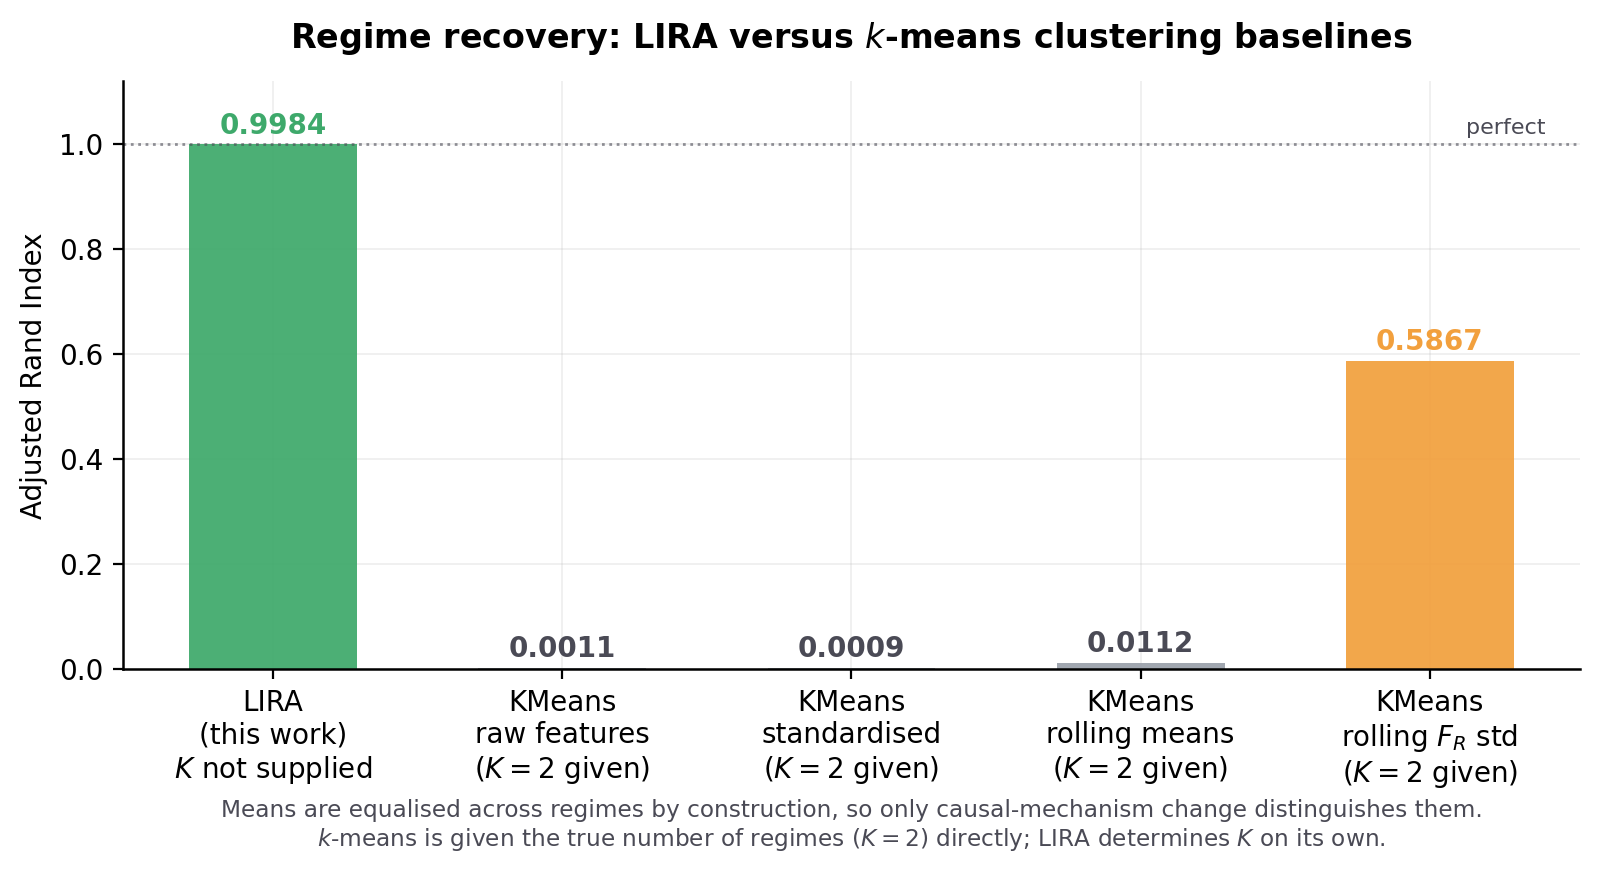
\includegraphics[width=\textwidth]{figs/fig08_baselines.png}
    \caption{Regime recovery: LIRA against structure-blind clustering baselines.}
    \label{fig:chapter5-8}
\end{figure}


\section{Structural coefficient recovery}

Fitting Equation~\eqref{eq:ch4-6} within each leaf recovers the generating coefficients
accurately and identifies the isolated variable in both regimes.

The recovered structural coefficients are reported in Table~\ref{tab:ch5-structural-coefficients}.



\begin{table}[htbp]
    \centering
    \small
    \caption{Recovered structural coefficients}
    \label{tab:ch5-structural-coefficients}
    \begin{tabularx}{\textwidth}{|>{\raggedright\arraybackslash}X|>{\raggedright\arraybackslash}X|>{\raggedright\arraybackslash}X|>{\raggedright\arraybackslash}X|>{\raggedright\arraybackslash}X|>{\raggedright\arraybackslash}X|>{\raggedright\arraybackslash}X|}
        \hline
          & \multicolumn{3}{c|}{Hard State} & \multicolumn{3}{c|}{Soft State} \\ \hline
        Coefficient & True & Recovered & Error & True & Recovered & Error \\ \hline
        $\beta_{L_X}$ & $+0.70$ & $+0.7172$ & $+0.017$ & $+0.18$ & $+0.1830$ & $+0.003$ \\ \hline
        $\beta_{\Gamma}$ & $-0.30$ & $-0.2989$ & $+0.001$ & $+0.20$ & $+0.2030$ & $+0.003$ \\ \hline
        $\beta_{T_{in}}$ & $0.00$ & $+0.0049$ & $+0.005$ & $-0.40$ & $-0.3894$ & $+0.011$ \\ \hline
        $\beta_{HR}$ & $-0.40$ & $-0.4015$ & $-0.002$ & $0.00$ & $-0.0070$ & $-0.007$ \\ \hline
        $\phi$ & $+0.50$ & $+0.4931$ & $-0.007$ & $+0.50$ & $+0.4958$ & $-0.004$ \\ \hline
    \end{tabularx}
\end{table}

The isolated coefficients are $+0.005$ in the Hard State and $-0.007$ in the Soft State.
Both are close to zero and much smaller than the active coefficients. The
autoregressive coefficient is recovered within $0.007$ of its true value.

\textbf{Temporal persistence.} The recovered $\phi$ values of $0.493$ and $0.496$ are
statistically indistinguishable, correctly reflecting that the generating process
assigns identical persistence to both regimes. The framework therefore does not
manufacture a persistence difference where none exists. It should be noted that the
abstract's claim regarding differential temporal persistence across accretion states is
a hypothesis about \textit{real} systems. The present synthetic design does not encode such a
difference, and testing it requires either a generator in which $\phi$ varies by regime
or application to observational data.


\subsection{The pooled-model baseline}

To test whether segmentation is necessary, we fit Equation~\eqref{eq:ch4-6} once
to the full series. The resulting structure matches neither regime.

The pooled and regime-specific estimates are compared in Table~\ref{tab:ch5-pooled}.



\begin{table}[htbp]
    \centering
    \small
    \caption{Pooled model versus regime-specific models}
    \label{tab:ch5-pooled}
    \begin{tabularx}{\textwidth}{|>{\raggedright\arraybackslash}X|>{\raggedright\arraybackslash}X|>{\raggedright\arraybackslash}X|>{\raggedright\arraybackslash}X|}
        \hline
        Coefficient & True (Hard) & True (Soft) & Pooled fit \\ \hline
        $\beta_{L_X}$ & $+0.70$ & $+0.18$ & $+0.2504$ \\ \hline
        $\beta_{\Gamma}$ & $-0.30$ & $+0.20$ & $-0.0285$ \\ \hline
        $\beta_{T_{in}}$ & $0.00$ & $-0.40$ & $-0.1167$ \\ \hline
        $\beta_{HR}$ & $-0.40$ & $0.00$ & $-0.1170$ \\ \hline
        $\phi$ & $+0.50$ & $+0.50$ & $+0.7650$ \\ \hline
    \end{tabularx}
\end{table}

Every coefficient is distorted. The coefficient on $\Gamma$ is negative in one regime
and positive in the other, but the pooled value is almost zero ($-0.029$). Both
isolated variables receive spurious coefficients. The autoregressive coefficient rises
from $0.50$ to $0.765$ because the pooled model attributes between-regime variation
to temporal persistence.

This result shows why a single pooled model can hide the coupling laws of distinct
accretion states.

The recovered and pooled coefficients are compared visually in Figure~\ref{fig:chapter5-7}.


\begin{figure}[htbp]
    \centering
    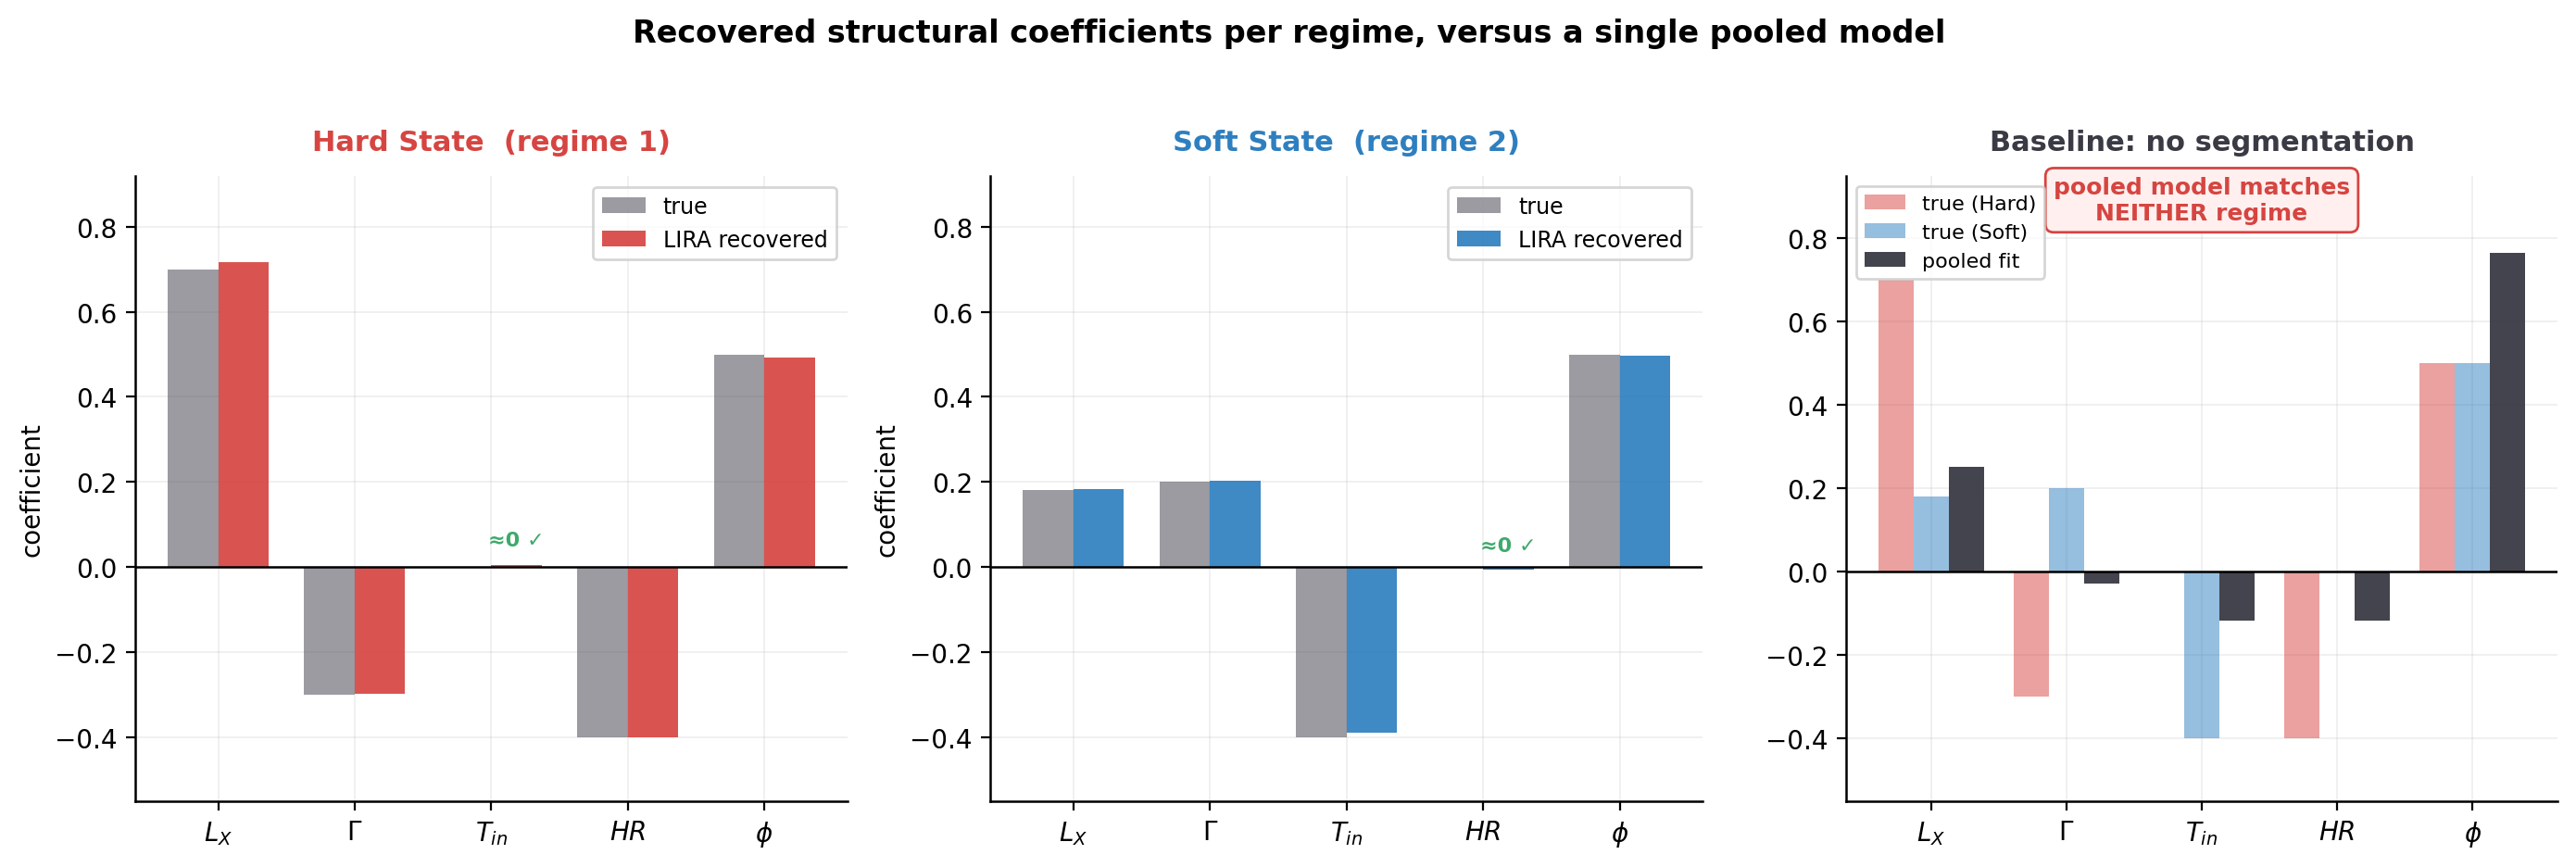
\includegraphics[width=\textwidth]{figs/fig07_coefficients.png}
    \caption{Recovered coefficients per regime, and the pooled model that matches neither.}
    \label{fig:chapter5-7}
\end{figure}


\section{Regime-specific causal graph recovery}

DYNOTEARS applied independently within each discovered leaf recovers the correct graph
structure in both regimes.

The contemporaneous and lagged edge estimates are reported in Tables~\ref{tab:ch5-contemporaneous}
and~\ref{tab:ch5-lagged}, respectively.



\begin{table}[htbp]
    \centering
    \small
    \caption{Contemporaneous edge recovery ($\hat{W}$)}
    \label{tab:ch5-contemporaneous}
    \begin{tabularx}{\textwidth}{|>{\raggedright\arraybackslash}X|>{\raggedright\arraybackslash}X|>{\raggedright\arraybackslash}X|>{\raggedright\arraybackslash}X|>{\raggedright\arraybackslash}X|}
        \hline
        Edge & Hard: true & Hard: $\hat{W}$ & Soft: true & Soft: $\hat{W}$ \\ \hline
        $L_X \to F_R$ & present $(+)$ & $+0.315$ yes & present $(+)$ & $+0.079$ yes \\ \hline
        $\Gamma \to F_R$ & present $(-)$ & $-0.100$ yes & present $(+)$ & $+0.090$ yes \\ \hline
        $T_{in} \to F_R$ & \textbf{absent} & \textbf{absent} yes & present $(-)$ & $-0.212$ yes \\ \hline
        $HR \to F_R$ & present $(-)$ & $-0.157$ yes & \textbf{absent} & \textbf{absent} yes \\ \hline
        any edge into $L_X$ & absent & absent yes & absent & absent yes \\ \hline
\end{tabularx}
\end{table}

Table~\ref{tab:ch5-contemporaneous} confirms the contemporaneous structure. The
active edges have the correct signs, the state-specific isolated variable is absent,
and $L_X$ has no contemporaneous parent.



\begin{table}[htbp]
    \centering
    \small
    \caption{Lagged edge recovery ($\hat{A}$, self-lags)}
    \label{tab:ch5-lagged}
    \begin{tabularx}{\textwidth}{|>{\raggedright\arraybackslash}X|>{\raggedright\arraybackslash}X|>{\raggedright\arraybackslash}X|>{\raggedright\arraybackslash}X|}
        \hline
        Self-lag & True & Hard: $\hat{A}$ & Soft: $\hat{A}$ \\ \hline
        $L_X$ & $0.90$ & $0.851$ & $0.851$ \\ \hline
        $\Gamma$ & $0.90$ & $0.854$ & $0.839$ \\ \hline
        $T_{in}$ & $0.90$ & $0.843$ & $0.838$ \\ \hline
        $HR$ & $0.90$ & $0.854$ & $0.847$ \\ \hline
        $F_R$ & $0.50$ & $0.527$ & $0.495$ \\ \hline
\end{tabularx}
\end{table}

Table~\ref{tab:ch5-lagged} reports the temporal self-lags. The four spectral
variables are recovered close to the generating value of $0.90$, while the radio
luminosity self-lag is close to $0.50$. Thus, the method recovers temporal dependence
as well as contemporaneous edges.

All edge signs are correct, the isolated variable is excluded in each regime, and
$L_X$ has no parent other than its own lag. The edge magnitudes are smaller than the
generating coefficients because of $L_1$ soft-thresholding. This does not change the
structural conclusions; unbiased effect magnitudes are estimated in Section~5.6.


\begin{figure}[htbp]
    \centering
    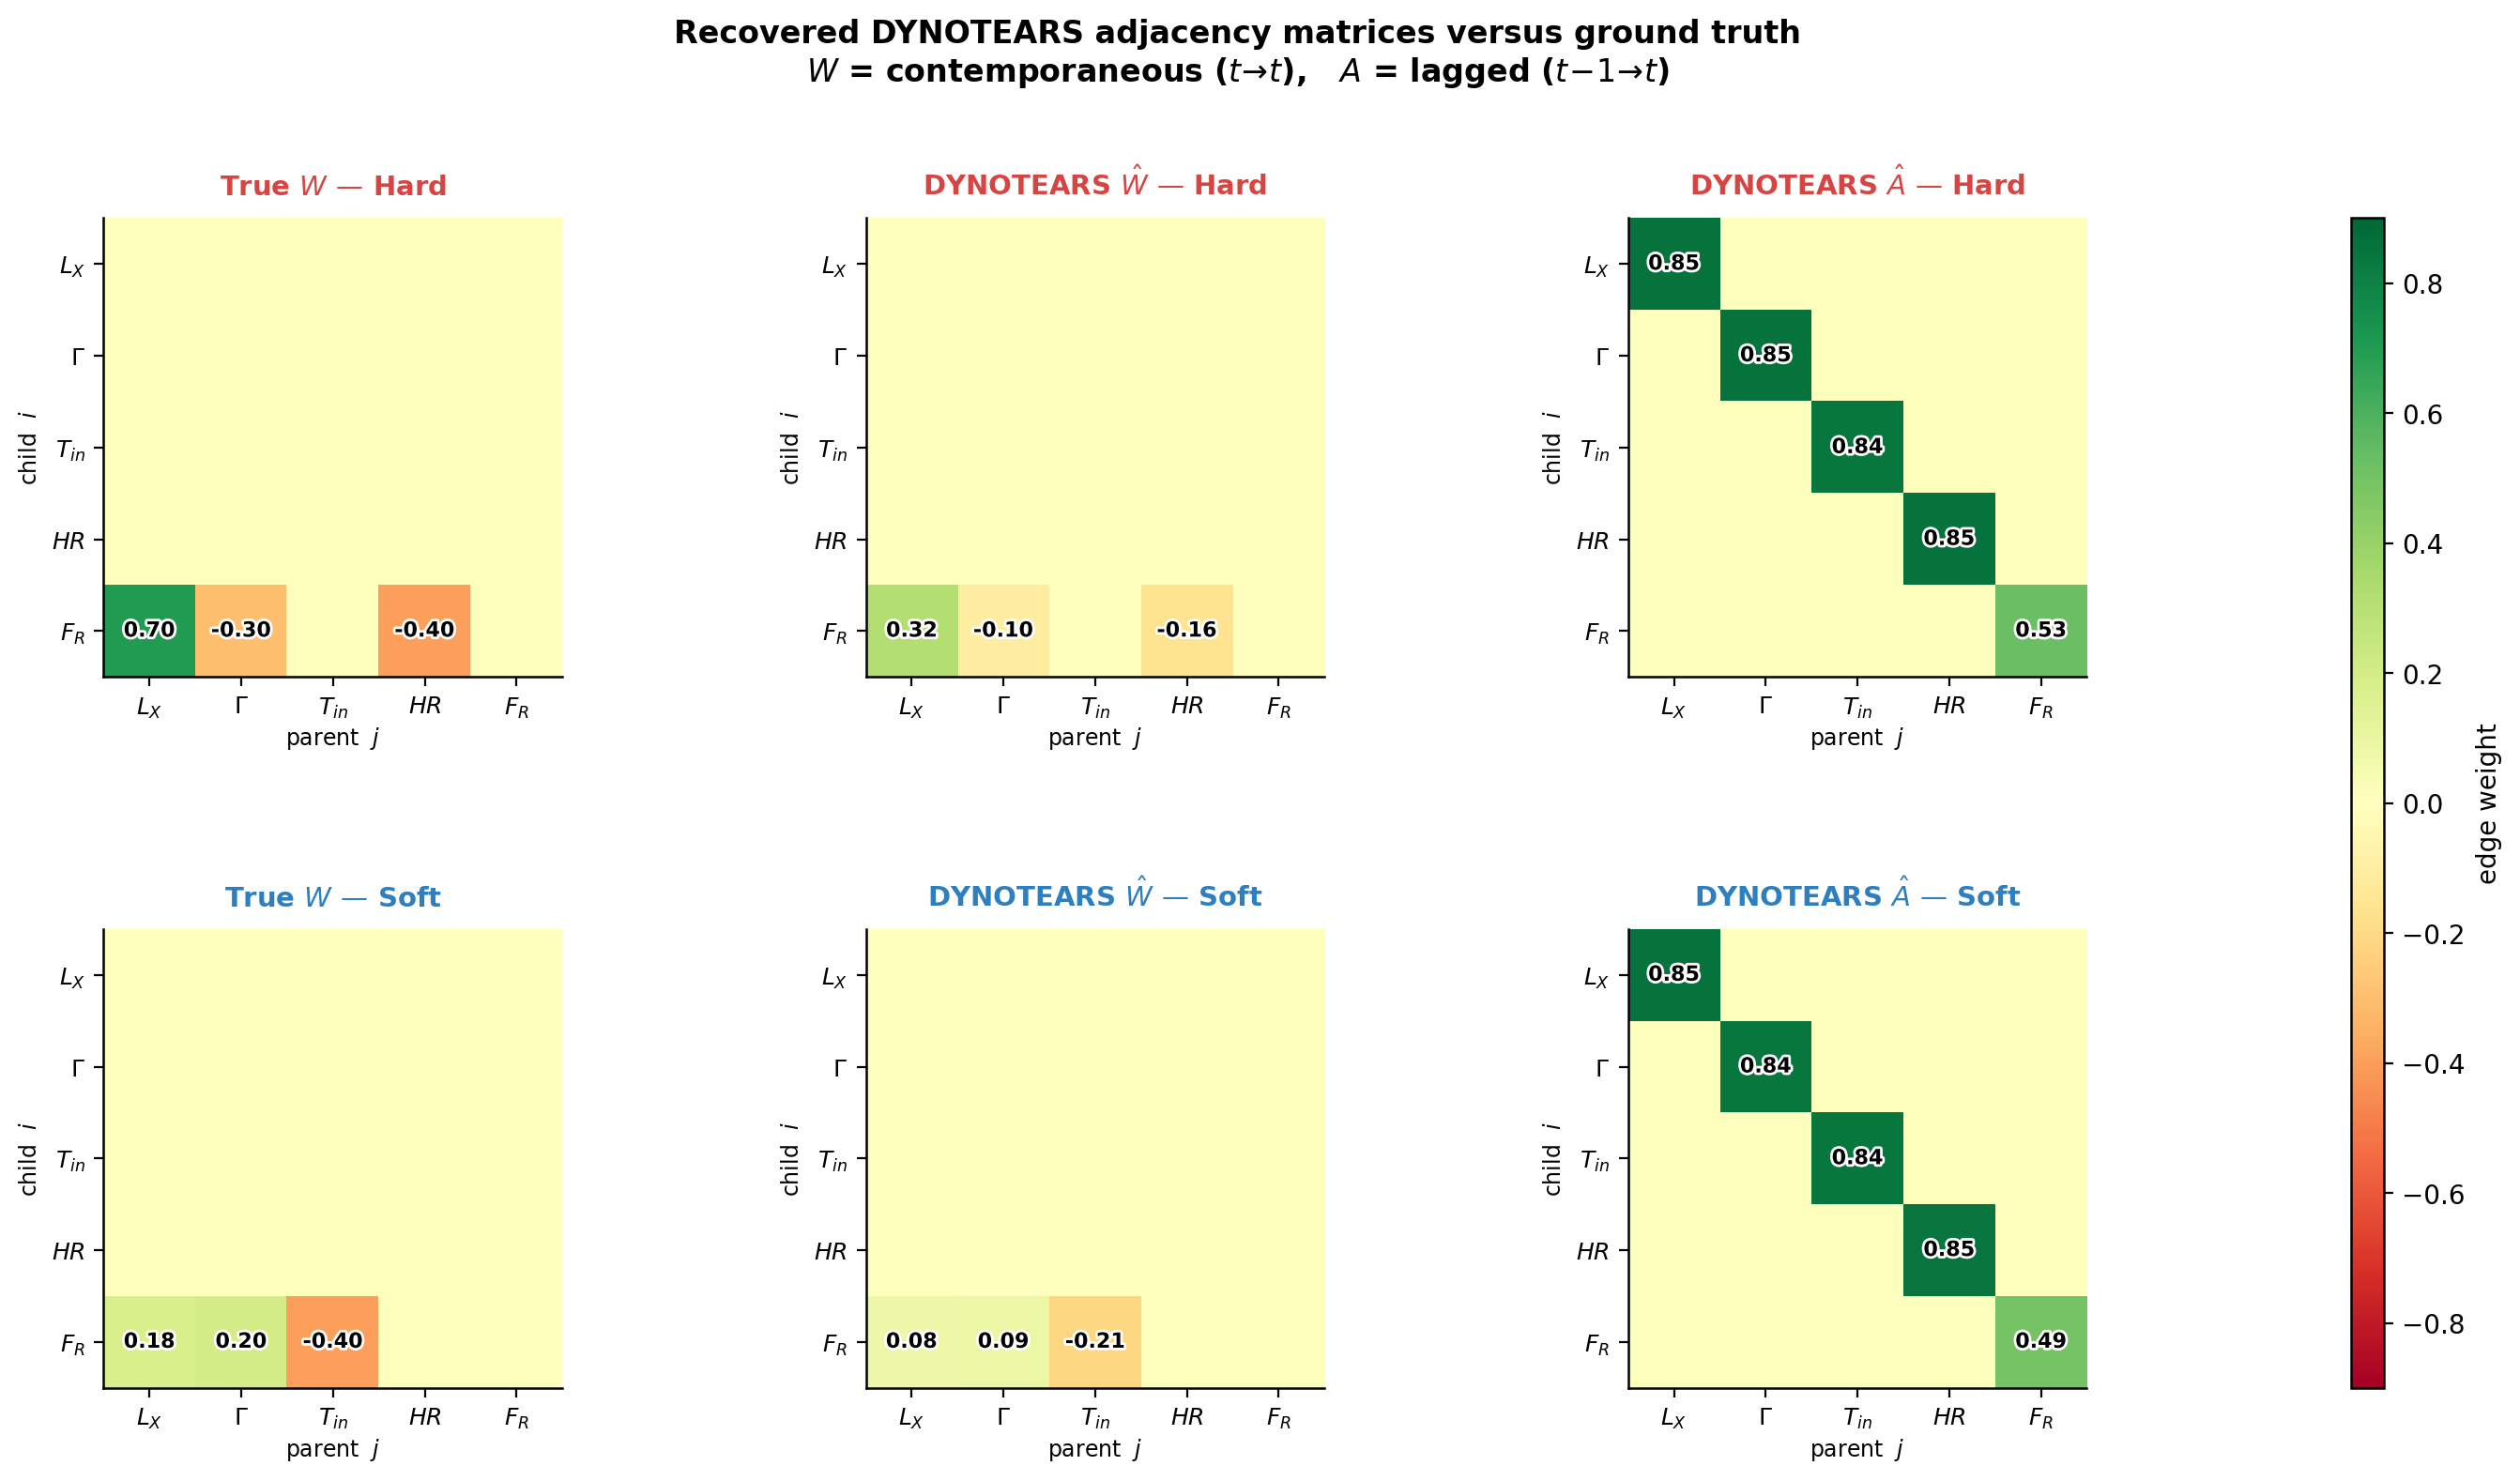
\includegraphics[width=\textwidth]{figs/fig09_adjacency.png}
    \caption{Recovered adjacency matrices against ground truth, for both the contemporaneous and lagged components.}
    \label{fig:chapter5-9}
\end{figure}

Figure~\ref{fig:chapter5-9} shows the same comparison in matrix form. The left
column is the true contemporaneous matrix $W$ for each regime. The middle column is
the recovered matrix $\hat{W}$, and the right column is the recovered lagged matrix
$\hat{A}$. In the Hard State the truth has three edges into $F_R$ and the recovery
selects the same three cells. In the Soft State the three active cells are different
and again all three are selected. The cells that are zero in the truth stay zero in
the recovery. The recovered edge weights are smaller than the true ones because of
the $L_1$ soft-thresholding in Stage 2. The lagged matrices are diagonal, so only
self-lags appear, and their entries are close to the generating values given in
Table~\ref{tab:ch5-lagged}. The pattern of edges, the signs of the edges, and the
isolated variable are therefore correct in both regimes.


\section{Causal effect estimation and validation}


\subsection{Effect estimates}

Backdoor adjustment with the remaining parents gives more accurate effect estimates
than the penalised Stage 2 weights, as expected from Section~4.8.

The estimated causal effects are listed in Table~\ref{tab:ch5-effects}.



\begin{table}[htbp]
    \centering
    \footnotesize
    \setlength{\tabcolsep}{4pt}
    \renewcommand{\arraystretch}{1.3}
    \caption{Estimated causal effects, refutation outcomes, and robustness}
    \label{tab:ch5-effects}
    \begin{tabularx}{\textwidth}{|>{\raggedright\arraybackslash}p{1.3cm}|>{\raggedright\arraybackslash}p{1.5cm}|>{\centering\arraybackslash}X|>{\centering\arraybackslash}X|>{\centering\arraybackslash}X|>{\centering\arraybackslash}X|>{\centering\arraybackslash}X|>{\centering\arraybackslash}X|}
        \hline
        Regime & Treatment & Estimate & True & \makecell{Random\\c.c.} & Placebo & Subset & Robustness \\ \hline
        Hard & $L_X$ & $+0.7111$ & $+0.70$ & $+0.7110$ & $+0.0016$ & $+0.7116$ & $+0.680$ \\ \hline
        Hard & $\Gamma$ & $-0.2964$ & $-0.30$ & $-0.2964$ & $-0.0003$ & $-0.2963$ & $+0.473$ \\ \hline
        Hard & $HR$ & $-0.3981$ & $-0.40$ & $-0.3981$ & $+0.0011$ & $-0.3985$ & $+0.556$ \\ \hline
        Hard & $F_R(t{-}1)$ & $+0.4983$ & $+0.50$ & $+0.4983$ & $-0.0006$ & $+0.4979$ & $+0.734$ \\ \hline
        Soft & $L_X$ & $+0.1799$ & $+0.18$ & $+0.1800$ & $-0.0006$ & $+0.1800$ & $+0.325$ \\ \hline
        Soft & $\Gamma$ & $+0.1994$ & $+0.20$ & $+0.1993$ & $-0.0005$ & $+0.1999$ & $+0.338$ \\ \hline
        Soft & $T_{in}$ & $-0.3833$ & $-0.40$ & $-0.3833$ & $-0.0001$ & $-0.3829$ & $+0.515$ \\ \hline
        Soft & $F_R(t{-}1)$ & $+0.5062$ & $+0.50$ & $+0.5063$ & $-0.0007$ & $+0.5059$ & $+0.728$ \\ \hline
    \end{tabularx}
\end{table}

Every estimate is within $0.017$ of its generating value. The random common-cause and
subset tests leave the estimates almost unchanged, while the placebo test reduces
every effect to within $0.002$ of zero.

The effect estimates and refutation outcomes are visualised in Figure~\ref{fig:chapter5-10}.

\begin{figure}[htbp]
    \centering
    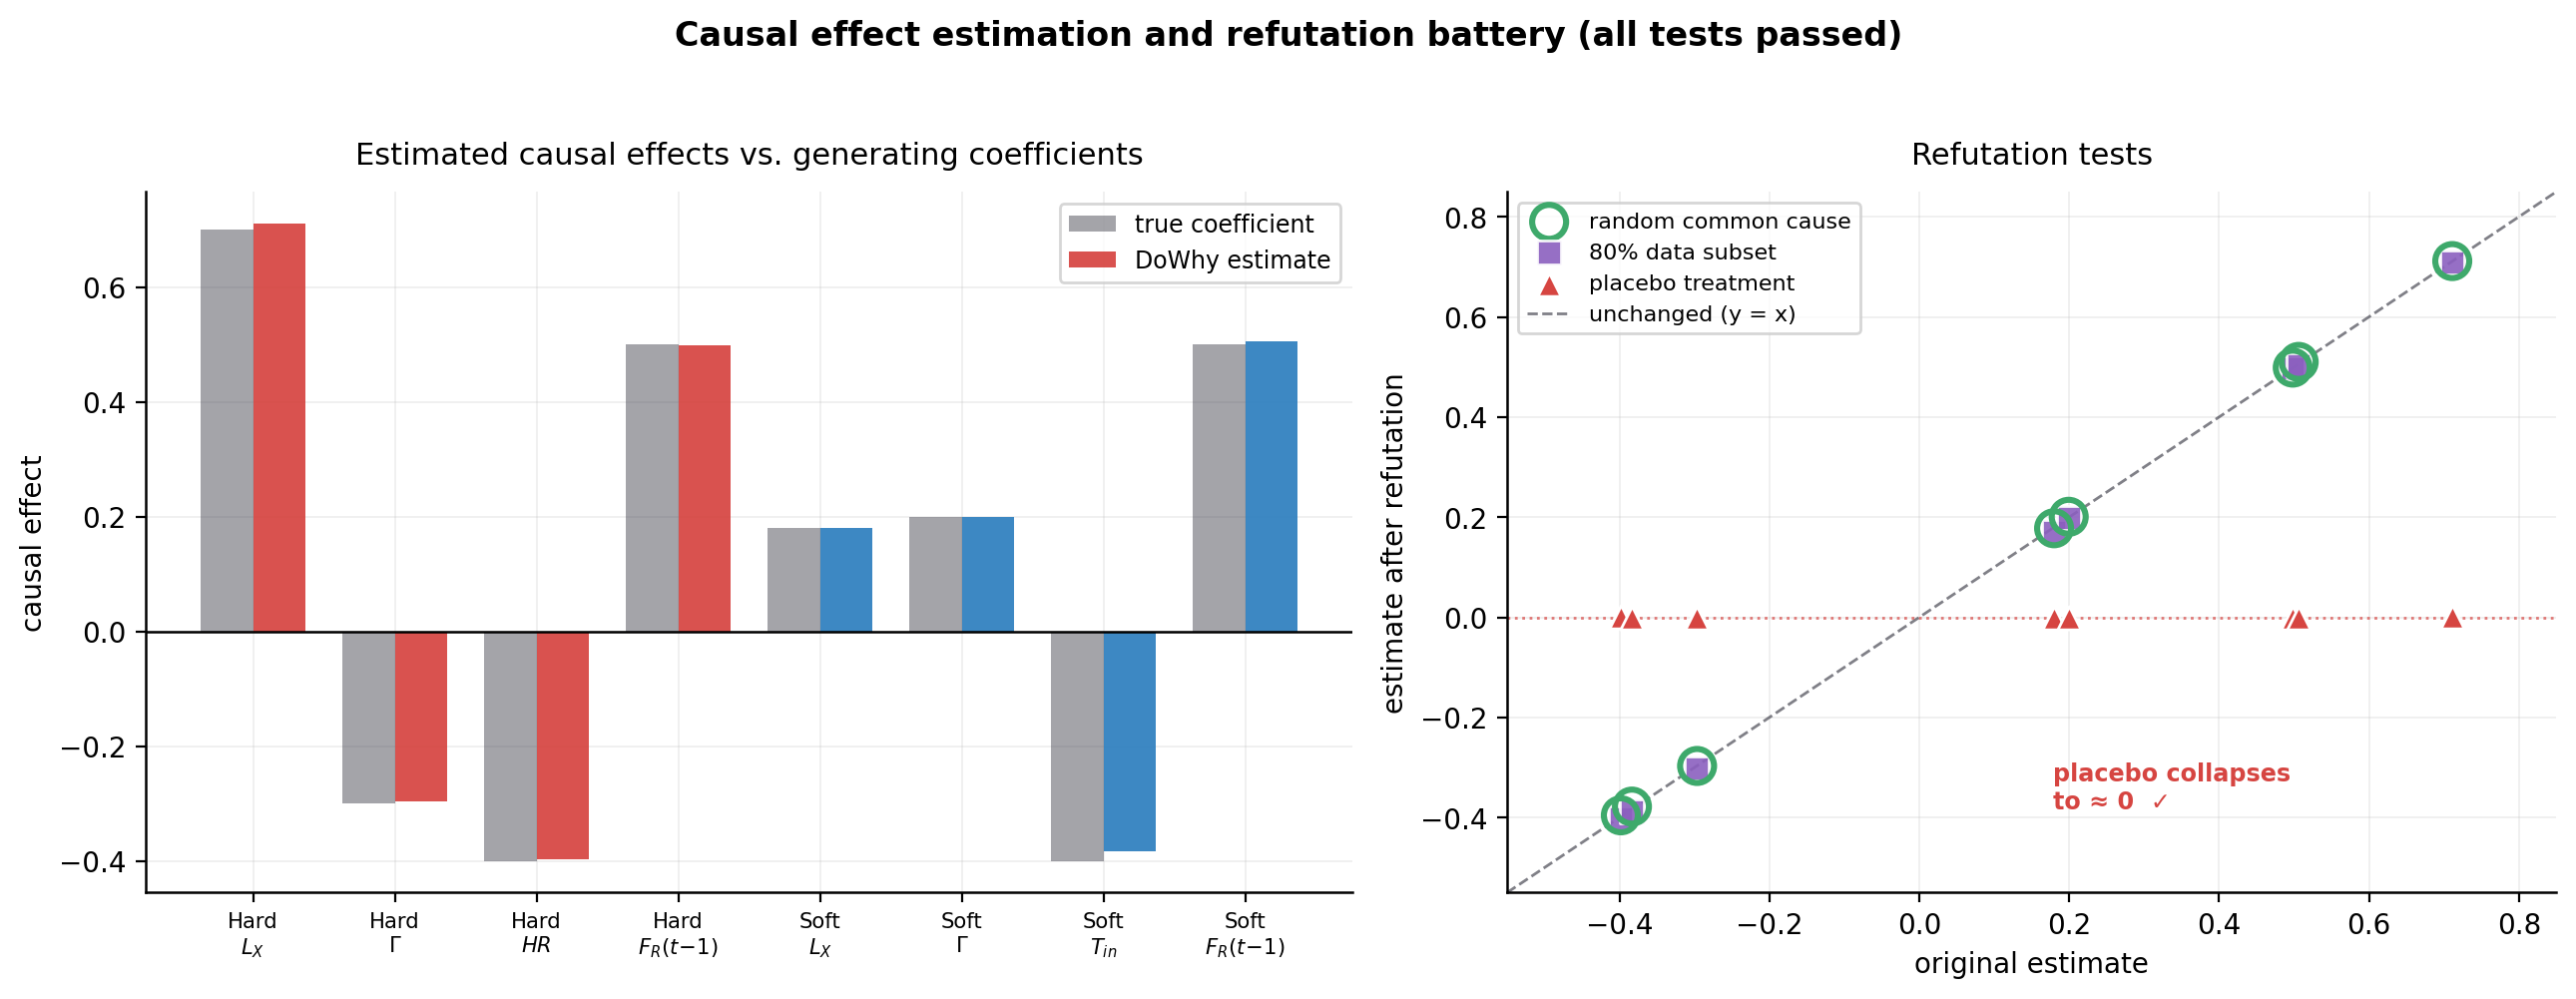
\includegraphics[width=\textwidth]{figs/fig10_effects_refutation.png}
\caption{Causal effect estimation and refutation battery. All reported tests pass.}
    \label{fig:chapter5-10}
\end{figure}

Figure~\ref{fig:chapter5-10} visualises these results. The left panel pairs each
estimated effect with the generating coefficient that produced it. The grey bar is
the true coefficient and the coloured bar is the estimate. The two bars have almost
the same height for every treatment. The right panel shows the three refutation
tests. Each point plots an estimate before refutation against the same estimate
after refutation. The random common-cause and subset points fall on the dashed
diagonal, so those refuters left the estimates unchanged. The placebo points fall on
the zero line instead, so the placebo treatment drove the estimate to zero. All
tests therefore pass.


\subsection{Sensitivity to unobserved confounding}

The Cinelli--Hazlett robustness value is the minimum residual variance that an
unobserved confounder must explain in both the treatment and the outcome to reduce an effect
to zero. Robustness increases with effect magnitude, with Pearson correlation
$r=0.888$. The weaker Soft State effects are therefore more sensitive to hidden
confounding and require more cautious interpretation.

\begin{figure}[htbp]
    \centering
    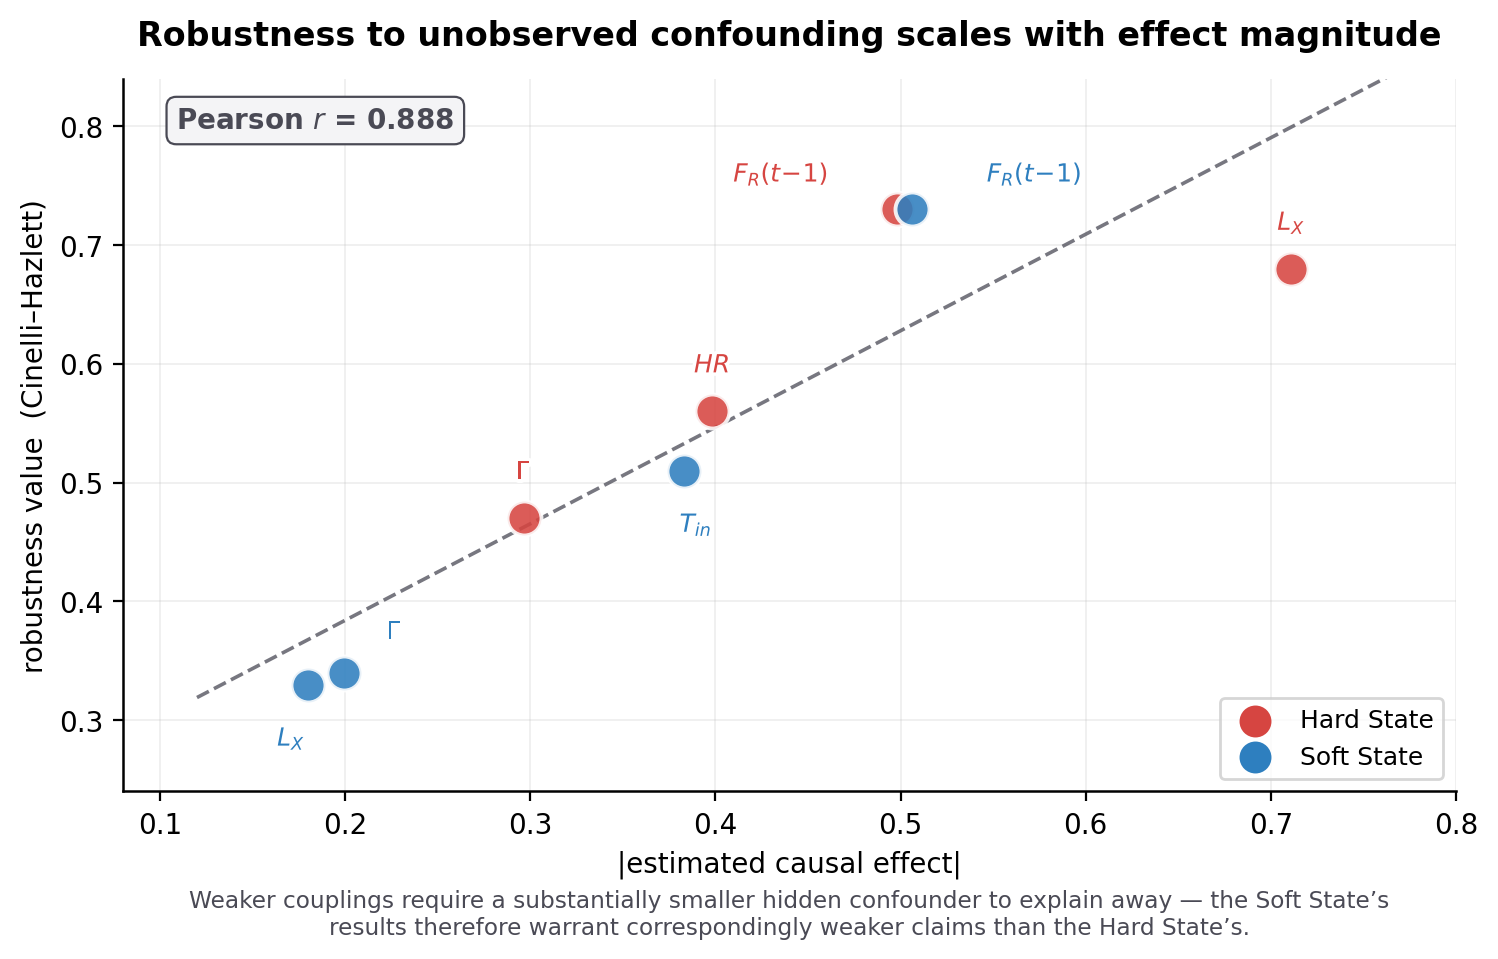
\includegraphics[width=\textwidth]{figs/fig11_robustness.png}
    \caption{Robustness to unobserved confounding as a function of estimated causal-effect magnitude.}
    \label{fig:chapter5-11}
\end{figure}

Figure~\ref{fig:chapter5-11} plots all eight effects of Table~\ref{tab:ch5-effects}
together. The horizontal axis gives the magnitude of each estimated effect and the
vertical axis gives its robustness value. Red points are Hard State effects and blue
points are Soft State effects. The points rise from the lower left to the upper
right. The dashed line is the linear fit through the points and the text box gives
the Pearson correlation of $r=0.888$. The two lowest points belong to the Soft
State $L_X$ and $\Gamma$ couplings. Their robustness values are near $0.33$, so a
confounder would have to explain about a third of the residual variance in both the
treatment and the outcome to erase them. The $F_R$ lag effects reach the highest
robustness values of $0.73$. The largest single effect, the Hard State $L_X$ coupling
at $0.71$, follows closely with $0.68$. An unobserved confounder would therefore have
to be strong to remove any of the eight effects. The weaker Soft State couplings need
the most caution because they can be removed by the weakest confounders.

\subsection{Graph falsification}

Falsification testing compares the conditional-independence implications of each
recovered DAG with randomly permuted graphs. With 20 permutations, neither DAG is
rejected at $\alpha=0.05$. One permutation falls within the Markov equivalence class
for each regime. The Hard State graph violates 15 of 22 local Markov conditions and
the Soft State graph violates 10 of 22; both outperform 95\% of the alternatives.

The falsification results are summarised in Table~\ref{tab:ch5-falsification}.

\begin{table}[htbp]
    \centering
    \small
    \caption{Graph falsification summary}
    \label{tab:ch5-falsification}
    \begin{tabularx}{\textwidth}{|>{\raggedright\arraybackslash}X|>{\centering\arraybackslash}X|>{\centering\arraybackslash}X|>{\centering\arraybackslash}X|>{\centering\arraybackslash}X|>{\raggedright\arraybackslash}X|}
        \hline
        Regime & LMC violations & Better than & Permutations in MEC & $p$ & Verdict \\ \hline
        Hard & 15 / 22 & 95.0\% & 1 / 20 & 0.05 & not rejected \\ \hline
        Soft & 10 / 22 & 95.0\% & 1 / 20 & 0.05 & not rejected \\ \hline
    \end{tabularx}
\end{table}

\textbf{Limitation.} With only 20 permutations, the $p$-value is restricted to
multiples of 0.05. The result is therefore indicative rather than conclusive. At
least 100 permutations should be used before publication.

\section{Summary of validation outcomes}

Table~\ref{tab:ch5-summary} consolidates the main validation outcomes.

\begin{table}[htbp]
    \centering
    \small
    \caption{Summary of experimental findings}
    \label{tab:ch5-summary}
    \begin{tabularx}{\textwidth}{|>{\raggedright\arraybackslash}p{3.4cm}|>{\raggedright\arraybackslash}X|>{\raggedright\arraybackslash}p{2.5cm}|}
        \hline
        Claim & Evidence & Outcome \\ \hline
        AR(1) term restores residual independence & Ljung--Box $p$: $<10^{-16} \to 0.211$ & confirmed (Section~5.2) \\ \hline
        Boundary is localised accurately & $\tau^* = 5004$ vs. true $5000$ & confirmed (Section~5.3.1) \\ \hline
        $K$ is determined automatically & $K = 2$ recovered, not specified & confirmed (Section~5.3.2) \\ \hline
        Both gates are necessary & Chow passes at both leaves, BIC rejects & confirmed (Section~5.3.2) \\ \hline
        Regimes are not separable by feature distribution & $k$-means (given $K=2$) ARI $\leq 0.012$ for three of four variants versus LIRA $0.998$ & confirmed (Section~5.3.3) \\ \hline
        Coefficients are recovered accurately & Maximum error $0.017$ across both regimes & confirmed (Section~5.4) \\ \hline
        Pooling produces a spurious structure & $\beta_\Gamma$ averaged to $-0.029$, $\phi$ inflated to $0.765$ & confirmed (Section~5.4.1) \\ \hline
        Regime-specific graphs are recovered & All signs correct, isolated variable excluded in each & confirmed (Section~5.5) \\ \hline
        Effects survive refutation & Placebo $<0.002$, other estimates unchanged & confirmed (Section~5.6.1) \\ \hline
        Robustness scales with effect size & $r = 0.888$ & confirmed (Section~5.6.2) \\ \hline
        Recovered graphs are not falsified & Neither rejected at $\alpha=0.05$ & indicative only (Section~5.6.3) \\ \hline
    \end{tabularx}
\end{table}

The table gives a compact view of the whole validation study. Each row states one
claim, the supporting evidence, and the section where the evidence is produced. Ten
of the eleven claims are confirmed by the experiments. The falsification claim is
marked indicative only because the test used 20 permutations. The other rows show
that every stage of the pipeline produced the expected result, from residual
cleaning to effect estimation.


\chapter{Conclusion}
This thesis introduced LIRA (Latent Invariant Regime Analysis), a framework for
finding hidden causal regimes in black hole accretion time series. The method uses
the power-law physics of the Fundamental Plane and models the observations with a
log-linear structural equation. Black hole mass is included in the intercept, while
four spectral-state variables describe changes over time. LIRA finds regime
boundaries through recursive partitioning, a lagged Chow $F$-test, and the Bayesian
Information Criterion. DYNOTEARS then estimates the causal graph inside each
regime. The results are checked with refutation tests, sensitivity analysis, and graph
falsification.

The synthetic experiments produced strong results. LIRA found the true boundary
within four observations out of ten thousand. It also found the correct number of
regimes. It recovered the structural coefficients to within $0.017$ of their true
values.

The isolated variable in each regime was identified correctly. Clustering methods
that ignored causal structure performed poorly. A pooled model also gave an averaged
structure that matched neither regime.

The two-gate design was useful. The Chow test alone would have created extra splits.
The BIC gate rejected those unnecessary splits.

Several limitations remain. The most important one is that every result in this
thesis was obtained from synthetic data. The synthetic experiments show that LIRA
works when the data follow the assumptions it was designed for. They do not show that
it works on real black hole observations.

Real X-ray light curves contain gaps. They also contain instrumental artefacts and
sources of variability that the generator does not reproduce. The pipeline may behave
differently once it is applied to them.

The simulation also uses the same linear and piecewise-stationary structure that LIRA
assumes during recovery. The tests are therefore favourable to the method by
construction.

Beyond the data itself, the model assumes linear and piecewise-stationary
relationships. Real accretion systems may change in nonlinear and continuous ways
instead. The identifiability result also depends on the collider structure used in
this thesis. It may not hold for a model with causal chains between the spectral
variables.

The sensitivity analysis showed that the weaker coupling in the Soft State supports
weaker causal claims than the Hard State.

The next step is to move from synthetic validation to real data. This is the single
most important piece of future work. Real observations are the only way to test
whether the regimes LIRA finds correspond to physical accretion states. They also
show whether the regimes are artefacts of the simulation.

The recommended sequence mirrors the phase structure used in this thesis. LIRA should
first be applied to well-monitored sources with dense coverage. GRS 1915+105 and
Cygnus X-1 are good candidates. Their known state transitions provide an external
check on the discovered boundaries.

The analysis should then be extended to the WATCHDOG catalogue. It offers a broader
sample of sources and longer baselines.

In both cases, the discovered regimes should be compared against independently
identified Hard and Soft States. The recovered causal graphs should be checked
against the physical expectations discussed in Chapter 2.

Any disagreement between the synthetic and real-data results should be treated as a
finding in its own right. It would locate exactly where the simulation assumptions
break down.

Other useful steps include testing nonlinear mechanisms. LIRA can also be compared
with CASTOR on the same benchmark. Future work can also allow causal structure to
change gradually rather than at fixed boundaries.

Together, these extensions would address the gap between the controlled synthetic
validation reported here and the noisier, less predictable behaviour of real
accretion systems.



\phantomsection
\printbibliography % Where the bibliography will be printed
\addcontentsline{toc}{chapter}{Bibliography}

% ********************************** Appendices ********************************
\begin{appendices} % Using appendices environment for more functionality
\newpage
\phantomsection
\addcontentsline{toc}{chapter}{Appendix A How to install \LaTeX}
\input{appendix/appendix_1}

\newpage
\phantomsection
\addcontentsline{toc}{chapter}{Appendix B Overleaf: GitHub for \LaTeX\ projects}
\input{appendix/appendix_2}
\end{appendices}

\end{document}
